\documentclass[type=master,twoside]{bithesis}

% 此处仅列出常用的配置。全部配置用法请见「bithesis.pdf」手册。
\BITSetup{
  cover = {
    %% 使用以下参数来自定义封面日期
    date = 2024年5月,
    autoWidthPadding = 0.25em,
  },
  info = {
    % 想要删除某项封面信息,直接删除该项即可。
    % 想要让某项封面信息留空(但是保留下划线),请传入空白符组成的字符串,如"{~}"。
    % 如需要换行,则用 “\\” 符号分割。
    classification = TQ028.1,
    UDC = 540,
    title = 面向代码克隆检测的多维源代码表征学习方法研究,
    % 如需覆盖竖排标题,请配置以下选项。
    % 下面的例子展示了如何在竖排标题中使用垂直或者旋转的英文。
    % verticalTitle = {形状记忆聚氨酯{L } {T } {X }的合成 \rotatebox[origin=c]{-90}{Feng Kaiyu} 及其在织物中的应用},
    titleEn = Research on Multidimensional Source Code Representation Learning Method for Code Clone Detection,
    author = 王丹,
    % 如果想要手动控制盲审模式下的隐藏信息,可以使用宏 \SecretInfo{}。使用方式有两种,如:
    % major = \SecretInfo{材料科学与工程} 可以得到 ******* (用等量的替换符号替代)
    % major = \SecretInfo{材料科学与工程}[ABCDEF] 可以得到 ABCDEF (用你自定义的内容替代)
    major = 计算机技术,
    school = 计算机学院,
    degree = 工学硕士,
    chairman = **教授,
    defenseDate = 2024年5月1日,
    supervisor = 马锐教授,
    authorEn = Dan Wang,
    schoolEn = Beijing Institute of Technology,
    supervisorEn = Associate Prof. Rui Ma,
    chairmanEn = Prof. **,
    degreeEn = Master of Science,
    majorEn = Computer Technology, 
    defenseDateEn = {May, 12th, 2024},
    keywords = {代码克隆检测;深度学习;代码表征学习},
    keywordsEn = Code cloning detections; Code representation learning; Deep learning
    % 必要时置于封面右上角,并按照国家规定进行标记。
    % classifiedLevel = 密级\BigStar 保密期限,
  },
  % 在目录页中不显示摘要和主要符号对照表的标题。
  TOC = {
    abstract = false,
    abstractEn = false,
    symbols = false,
  },
  style = {
    pageVerticalAlign = scattered,
    % 开启 Windows 平台下的中易宋体伪粗体。
    % windowsSimSunFakeBold = true,
  },
  publications = {
    % 以下两个选项将影响「攻读学位期间发表论文与研究成果清单」中名称列表的省略阈值。
    % 一般来说,如果你在全部文献中最低排在第四位,建议你将两个值都设置为 4。
    % 更详细的说明请见手册。
    maxbibnames = 3,
    minbibnames = 1,
  },
  % 采用章节标题级别的附录格式
  appendices / chapterLevel = true,
  const = {
    % 由于现存的 Word 模板、旧有 LaTeX 模板与《北京理工大学研究生学位论文撰写规范》的规定不一致,
    % 论文封面的某些字段内容需要用户根据自己的情况进行手动调整。
    % 目前给出的默认值是按照 2018 年发布的《北京理工大学研究生学位论文撰写规范》中的要求进行设置的。
    % 比如注释掉的这一行:将会修改封面中的「申请学位级别」为「申请学位」。
    % info / degree = {申\quad{}请\quad{}学\quad{}位},
    % info / major = {学\quad{}科\hspace{5pt}/\hspace{5pt}类\quad{}别}
  }
}

% 大部分关于参考文献样式的修改,都可以通过此处的选项进行配置。
% 详情请搜索「biblatex-gb7714-2015 文档」进行阅读。
\usepackage[
  defernumbers=true,
  backend=biber,
  style=gb7714-2015,
  gbalign=gb7714-2015,
  gbnamefmt=lowercase,
  gbpub=false,
  gbannote=true,
  gbpunctin=false,
  doi=false,
  url=false,
  eprint=false,
  isbn=false,
]{biblatex}

% 添加参考文献
\addbibresource{reference/main.bib}
% 攻读学位期间发表论文与研究成果清单,详细使用方法见 `chapters/pub.tex`。
\addbibresource{reference/pub.bib}


\usepackage{graphicx}

\usepackage{url}
\usepackage{float}
\usepackage{amsmath}
\nocite{*}
\usepackage{multirow}

\begin{document}

% 封面绘制
\MakeCover

% 打印书脊
\MakePaperBack

% 中文信息与英文信息
\MakeTitle

% 论文原创性声明和使用授权
\MakeOriginality

%%%%%%%%%%%%%%%%%%%%%%%%%%%%%%
%% 前置部分
%%%%%%%%%%%%%%%%%%%%%%%%%%%%%%
\frontmatter

% 摘要
\begin{abstract}
  代码克隆检测是软件工程领域的重要任务,如何对源代码进行表征学习决定了对源代码信息抽取程度,进而影响下游任务的检测精度。现有的代码表征学习方法存在对代码结构信息和语义信息利用不充分的问题。基于此,本文提出了一种面向代码克隆检测的多维源代码表征学习方法RLCCD(Code \textbf{R}epresentation \textbf{L}earning for \textbf{C}ode \textbf{C}lone \textbf{D}etection),构建词法单元Token、抽象语法树AST、程序依赖图PDG三个不同维度的代码表征模型,通过特征融合得到多维特征,实现对代码信息的充分利用。
  
  在词法单元Token维度,针对现有Token方法在模型训练中经常出现的集外词问题,提出基于预训练辅助模型的Token表征学习方法。通过组合Token序列的相邻单元,不断迭代,更新词汇表。在Token维度表征阶段使用双向长短期记忆网络BiLSTM模型,从前后两个方向同时捕获序列的语义信息,提高对代码信息的表征程度。
  
  在抽象语法树AST维度,针对现有AST方法将抽象语法树转化为二叉树过程中破坏原有结构,增加树高度,导致模型训练过程中梯度消失的问题,提出基于子树划分的抽象语法树表征学习方法。其中,通过子树划分得到AST序列,输入基于树的卷积神经网络学习得到子树粒度的代码信息,输入双向GRU模型学习得到整个抽象语法树的嵌入表征,从而提高树维度的代码表征能力。

  在程序依赖图PDG维度,针对现有PDG方法将代码片段表征为有向多重图,采用子图匹配算法所消耗的时间、空间开销巨大的问题,提出基于图过滤的程序依赖图表征学习方法。在图表征阶段之前,针对候选程序依赖图对集合进行图过滤减少模型输入规模,提升后续基于图卷积神经网络进行图表征学习的训练效率。

  最后,针对以上三个单维度对代码信息利用不充分的问题,提出基于多模态学习的特征融合方法,通过特征连接Concat、特征加法Add两种方式得到混合特征,实现多维源代码表征学习。为验证本文所提方法RLCCD的有效性,与SourcererCC、ASTNN、CCSharp、SCDetector四种代码克隆工具进行对比试验,结果表明,RLCCD可以利用Token、AST、PDG 三个维度数据之间的信息互补性,学习到更好的特征表示,代码信息利用率高,有效提高了下游代码克隆检测任务的精度。

\end{abstract}

\begin{abstractEn}

  Code cloning detection is an important task in the field of software engineering. How to represent and learn source code determines the degree of information extraction from source code, which in turn affects the detection accuracy of downstream tasks. The existing code representation learning methods suffer from insufficient utilization of code structure and semantic information. Based on this, this paper proposes a multi-dimensional source code representation learning method for code cloning detection(RLCCD), constructing code representation models with three different dimensions: lexical unit Token, abstract syntax tree AST, and program dependency graph PDG. Through feature fusion, multi-dimensional features are obtained, achieving full utilization of code information.


  In terms of Token dimension, a token representation learning method based on pre trained auxiliary models is proposed to address the common problem of out of set words in existing token methods during model training. By combining adjacent units of the Token sequence, iterating continuously, and updating the vocabulary. In the token dimension representation stage, a bidirectional long short-term memory network BiLSTM model is used to capture the semantic information of the sequence from both the front and back directions simultaneously, improving the degree of representation of code information.

  In terms of AST dimension, a representation learning method for abstract syntax trees based on subtree partitioning is proposed to address the problem of existing AST methods breaking the original structure, increasing tree height, and causing gradient disappearance during model training. Among them, the AST sequence is obtained through subtree partitioning, the code information at the subtree granularity is learned by inputting a tree based convolutional neural network, and the embedding representation of the entire abstract syntax tree is learned by inputting a bidirectional GRU model, thereby improving the code representation ability of the tree dimension.

  In terms of PDG dimension, a graph filtering based program dependency graph representation learning method is proposed to address the significant time and space cost of using subgraph matching algorithms to represent code fragments as directed multiple graphs in existing PDG methods. Before the graph representation stage, filter the set of candidate program dependency graphs to reduce the input size of the model and improve the training efficiency of graph representation learning based on graph convolutional neural networks.

  Finally, in response to the problem of insufficient utilization of code information in the above three dimensions, a feature fusion method based on multimodal learning is proposed, which obtains mixed features through feature concatenation and feature addition, achieving multi-dimensional source code representation learning. To verify the effectiveness of the proposed method RLCCD, a comparative experiment was conducted with four code cloning tools, namely Source rCC, ASTNN, CCSharp, and SCDetector. The results showed that RLCCD can utilize the information complementarity between Token, AST, and PDG dimensions of data to learn better feature representations. The code information utilization rate is high, effectively improving the accuracy of downstream code cloning detection tasks.

\end{abstractEn}


% 制作目录
\MakeTOC

% 插图目录
\listoffigures
% 表格目录
\listoftables

% 主要符号对照表
% %%
% The BIThesis Template for Graduate Thesis
%
% Copyright 2020-2023 Yang Yating, BITNP
%
% This work may be distributed and/or modified under the
% conditions of the LaTeX Project Public License, either version 1.3
% of this license or (at your option) any later version.
% The latest version of this license is in
%   http://www.latex-project.org/lppl.txt
% and version 1.3 or later is part of all distributions of LaTeX
% version 2005/12/01 or later.
%
% This work has the LPPL maintenance status `maintained'.
%
% The Current Maintainer of this work is Feng Kaiyu.

\begin{symbols}
  \item[BIT] 北京理工大学的英文缩写
  \item[\LaTeX] 一个很棒的排版系统
  \item[\LaTeXe] 一个很棒的排版系统的最新稳定版
  \item[ctex] 成套的中文\LaTeX{}解决方案,由一帮天才们开发
  \item[$ e^{\pi{}i}+1=0$] 一个集自然界五大常数一体的炫酷方程
\end{symbols}


\mainmatter

% 请根据论文内容,按照顺序添加章节。
\chapter{绪论}
\label{chap:intro}

\section{研究背景与意义}
\label{sec:background}
代码克隆,也叫代码复用,是指在软件系统中存在两个或两个以上的相似代码片段\cite{乐乔艺2021代码克隆检测研究进展综述},是软件开发中的常见现象。随着互联网时代的发展,网络上各种开源项目越来越多样化,获取也更加便利。许多企业通过软件资源库、外部开源软件、软件产品线及开发框架等方式建立了多种多样的软件复用开发方法,同时开发人员自身也会通过多种方式大量复用已有的软件资源。在这些软件复用方法和资源的支持下,软件系统和软件产品大量引入了开源软件、网络资源、商业软件等第三方代码成分。这些第三方代码在多个软件系统中复制、传播和演化,给软件系统带来了软件质量的不确定性和风险,甚至导致漏洞的传播。

近年来,第三方代码中包含的漏洞数量呈现出快速增长的趋势。根据美国新思科技公司(Synopsys, Inc.)发布的《2023年开源安全和风险分析报告》\cite{Synopsys_2023}显示,在2022年审计的1703个代码库中,98\%的项目都包含开源代码,84\%的代码库包含至少一个已知开源漏洞,比2022年版的报告中增加了近4\%,有48\%代码库中包含高风险漏洞。
图\ref{fig:Proportion}统计了2018年至2022年Synopsys审计代码库中开源代码及漏洞占比,从图\ref{fig:Proportion}中可以看出开源代码及漏洞数量整体呈上升趋势。

\begin{figure}[H]
    \centering
    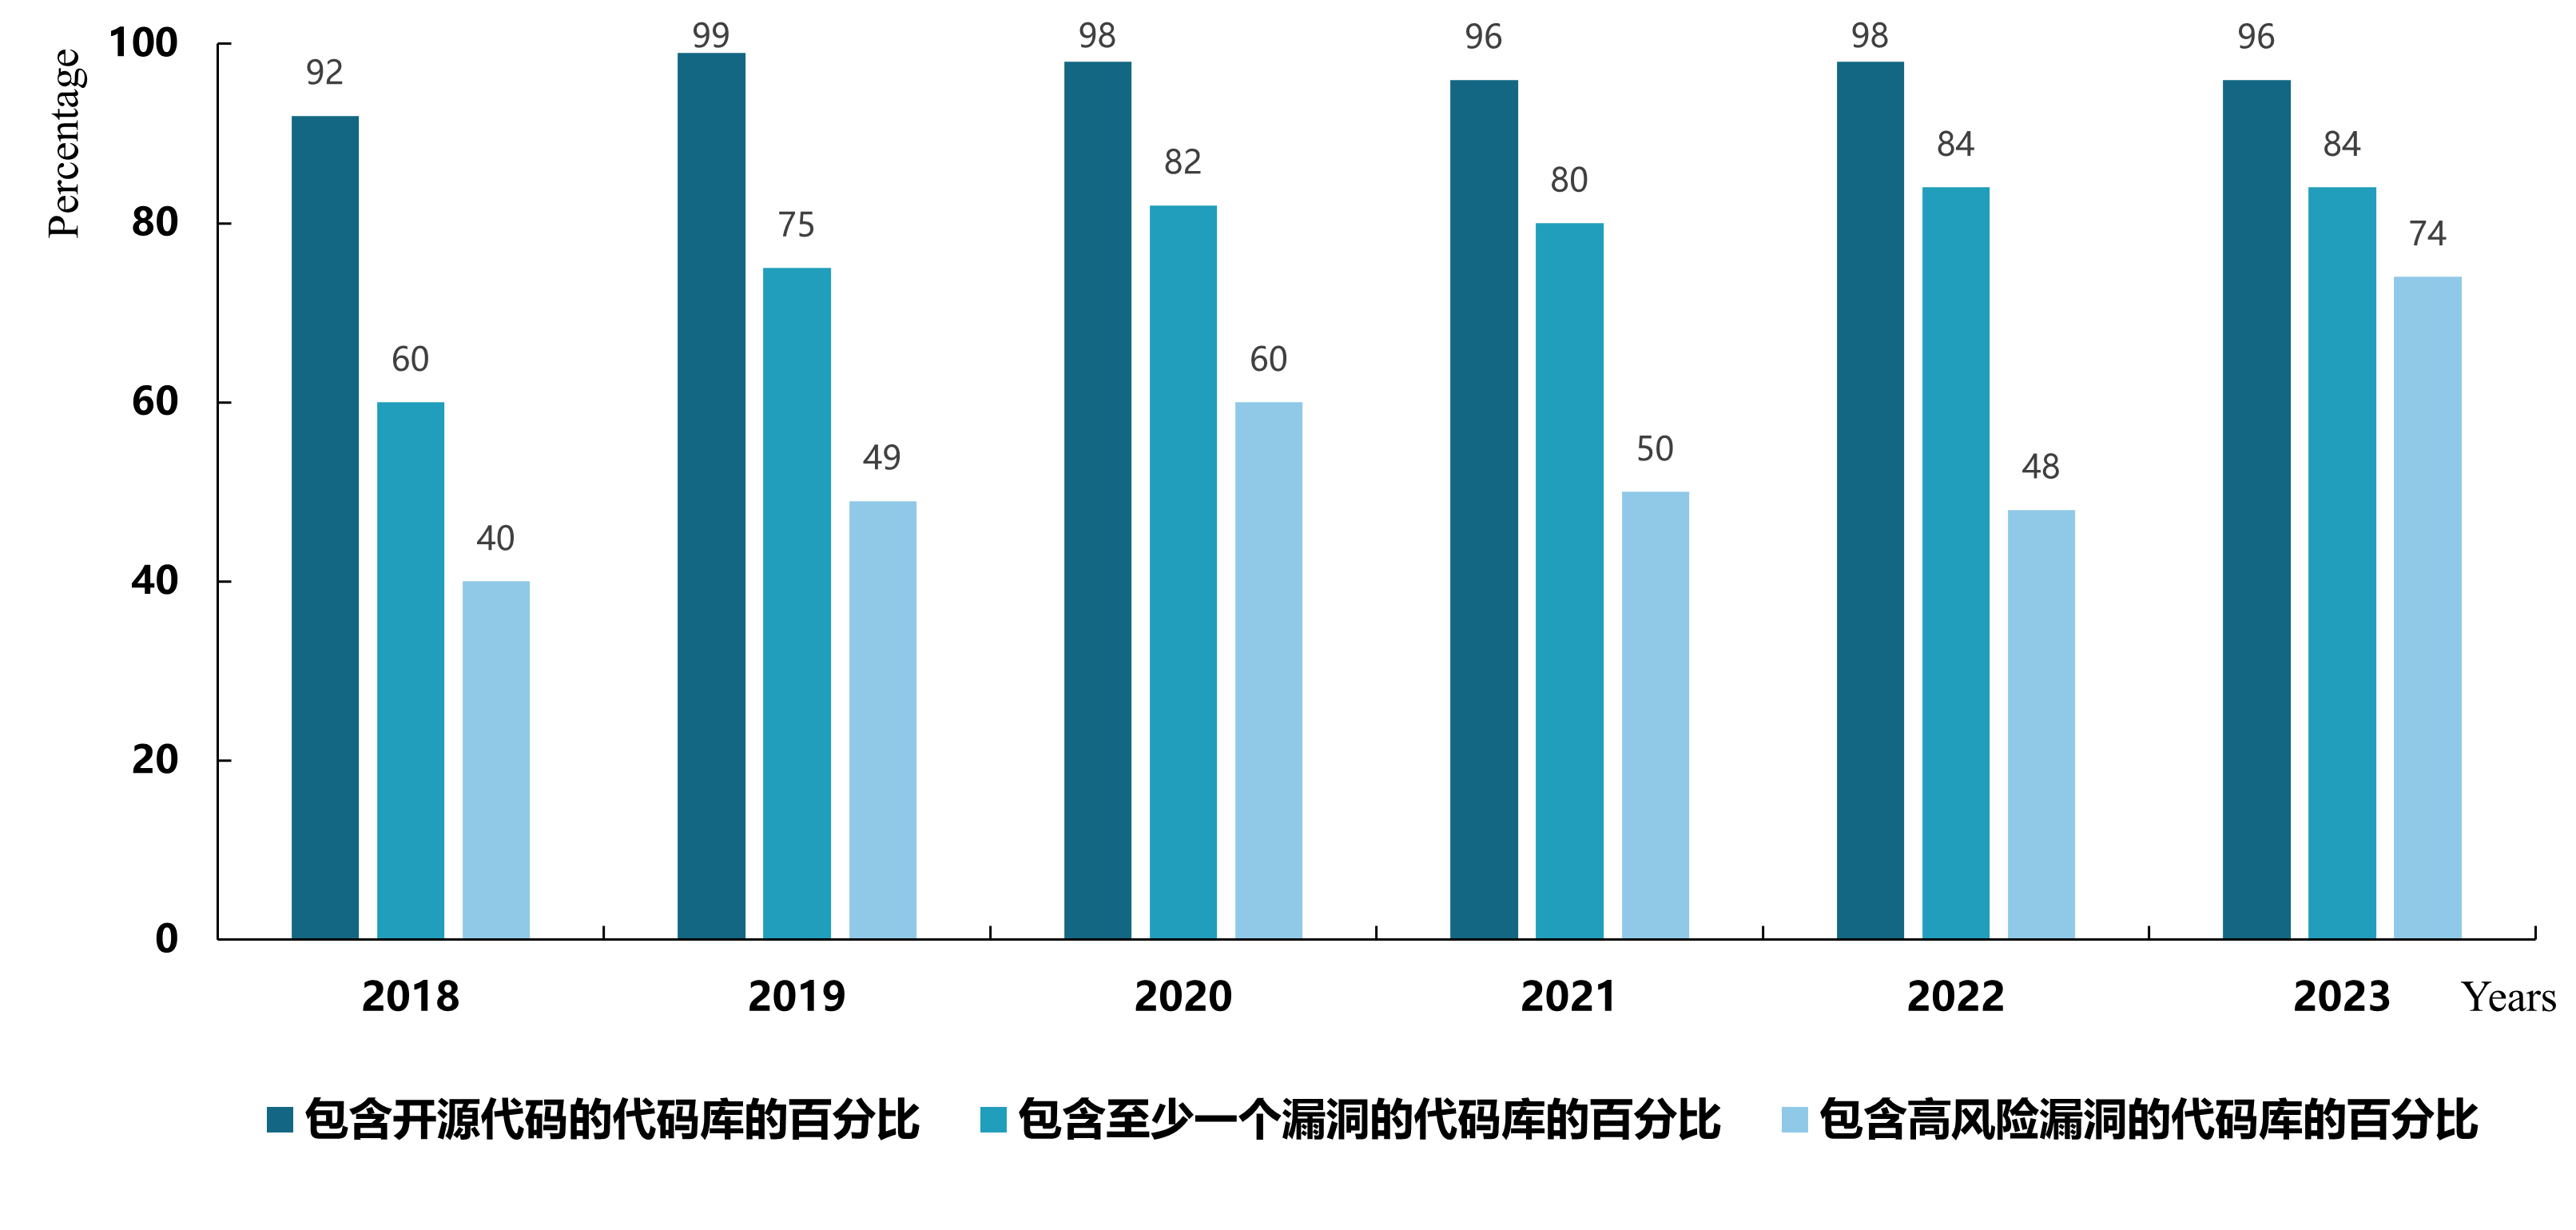
\includegraphics[width=0.85\textwidth]{figures/Proportion}
    \caption{2018-2022年Synopsys审计代码库中的开源代码及漏洞占比示意图}\label{fig:Proportion}
\end{figure}

同时,Synopsys统计了包含易受攻击组件的代码库占比,其中使用JQuery 和 Lodash 两个最流行的开源组件的代码库占比达到了47\%和 31\%,其余组件占比如图\ref{fig:assembly}所示。一旦易受攻击组件出现安全问题,通常会导致软件遭受供应链攻击。据Gartner\cite{Gartner_2022}预测,到2025年,全球45\%的组织将遭受软件供应链攻击,比2021年增加三倍。因此,准确地检测代码克隆对于软件开发和维护是至关重要的。

\begin{figure}[H]
    \centering
    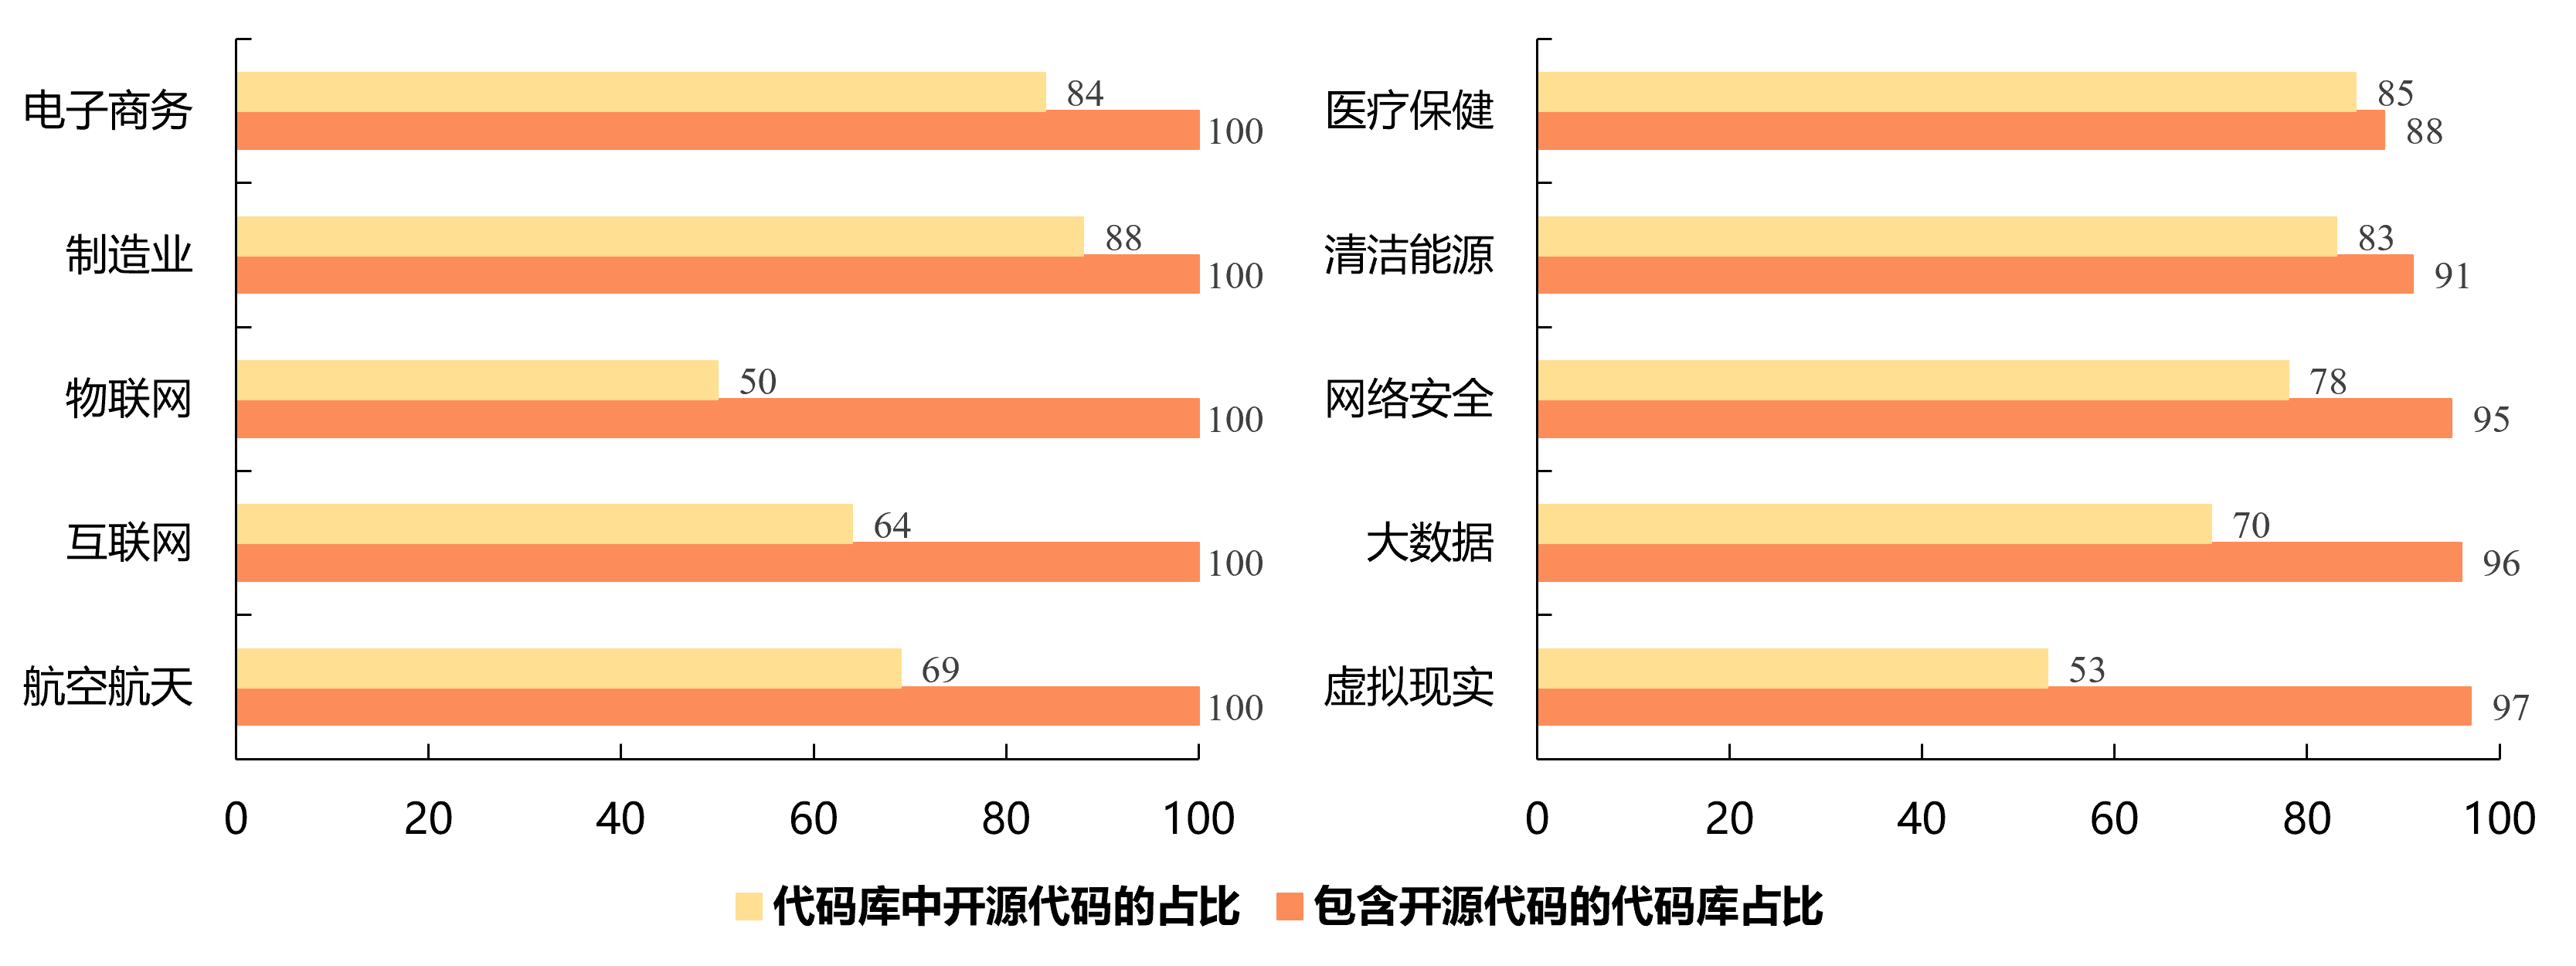
\includegraphics[width=0.85\textwidth]{figures/assembly}
    \caption{2022年Synopsys审计代码库中包含易受攻击组件的百分比示意图}
    \label{fig:assembly}
\end{figure}

早期进行代码克隆检测通常采用人工检查并标注的方法,通过收集整理大量的代码逐行检查语法、语义结构,由人工复查筛选出正确的克隆代码并对其进行标注,由此形成了早期的代码克隆数据样本,例如,2015年Svajlenko\cite{7332459}等人提出了著名评估基准集BigcloneBench,该数据集是由克隆领域三个专家评委花费216小时通过人工验证的方法从IJaDataset\cite{IJaDataset2.0}中挖掘而来,总数据量达到800万,其背后的人工花费巨大。但利用人工的方法检测代码克隆效率低,成本高,并且无法保证准确率\cite{7965429},因此,有研究人员提出代码克隆检测技术,目的在于自动化定位软件系统中的代码克隆,并能够节约成本,减少出错风险\cite{Yang2015ClassificationMF}。

早期代码克隆检测技术通常将代码视为自然语言文本进行处理,通过文本相似性判断代码相似程度;随着编译技术的发展,研究者们将编译原理中的词法分析技术运用到代码克隆检测领域;近年来,基于多维源代码表征学习的代码克隆检测技术已经引起了学者们广泛的兴趣,有研究人员从代码克隆检测与代码表征学习技术相结合这一方面进行了探索,试图从关键技术点入手,找到合适的结合点,以提高定代码克隆检测技术的效率和智能化程度。


\section{研究现状与趋势}
\label{sec:status}

\subsection{代码克隆检测技术}
\label{subsec:Code clone detection}

代码克隆检测技术,旨在自动化定位软件系统中的代码克隆,节省成本,减少出错风险,有助于更好地保证软件质量。目前已有的代码克隆方法大多需要对代码片段进行信息抽取,转换为中间表征,然后根据表征方式的不同计算不同代码片段之间的相似度,完成克隆检测任务。其具体流程如图\ref{fig:figure1}所示。
\begin{figure}[H]
    \centering
    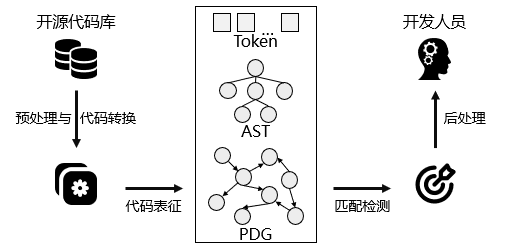
\includegraphics[width=0.95\textwidth]{figures/figure1}
    \caption{代码克隆检测流程}\label{fig:figure1}
\end{figure}

从图\ref{fig:figure1}可以看出一个完整的代码克隆检测过程通常包括预处理与转换、代码表征、匹配检测、后处理几个阶段。具体而言,一般的代码克隆检测从代码预处理与转换开始,首先删除与检测无关的空白行、注释、缩进等元素,并根据检测粒度将源代码划分为单独的片段,比如类、函数等;然后在代码表征步骤,将比较单元转换为相应的中间表示,常见的中间表示有:词法单元(Token)、抽象语法树(abstract syntax tree,AST)、程序依赖图(Program dependency graph,PDG)等;在匹配检测阶段,将根据得到不同的中间表示采用相应的匹配算法进行相似度计算,例如抽象语法树的比较通常采用子树匹配算法,程序依赖图的比较则采用子图同构算法。此阶段将代码片段两两对比,以查找相似代码源片段,得到代码克隆对。最后在后处理阶段,通常会通过人工检测或者算法过滤掉错误的代码克隆,并以适当的方式呈现给开发人员提供帮助。

在这些步骤中,代码表征方式决定了匹配检测方法的预处理方式、模型设计、部署方式、运行效率,并影响最终结果\cite{陈秋远2019代码克隆检测研究进展}。比如将源代码表征为文本,其预处理过程主要为去除噪声,如空格、注释等,其比较算法可以利用文本相似的一系列方法,能够检测到语法相似的克隆代码;而如果表征为抽象语法树,则其预处理过程需要解释器的参与,相似比较算法更多地考虑了结构相似等,能够检测到语法层面相似的代码克隆。因此, 代码表征方式是代码克隆检测的关键步骤。


\subsection{代码表征学习}
\label{subsec:Code representation}
表征学习是指学习数据的表示,使其在构建分类器或其他预测因子时更容易提取有用信息\cite{Bengio2013Representation}。代码表征学习是对源代码的语义和语法信息进行表征,得到源代码的特征向量,并将其应用在不同的下游任务上。在代码克隆检测中,代码表征学习可以用来提取代码片段更高层次的抽象特征表示,这些特征表示能够捕捉代码的语法、语义以及结构信息。通过学习到的代码表征,可以更准确地比较和识别不同代码片段之间的相似性,从而实现克隆代码的检测和管理,提高检测的准确性和鲁棒性。因此,代码表征学习为代码克隆检测提供了重要的技术支持。

代码表征学习工作最早可追溯到100年前,基于传统机器学习的数据特征学习被广泛提出,主成分分析PCA(Principal Component Analysis)\cite{WOS:000202849800065}、线性判别分析LDA(Linear Discriminant Analysis)\cite{2012THE}都是经典的表征学习方法。随着神经网络的不断发展,基于深度学习的代码表征学习工作研究能够更有效地提取数据的特征,用于后续的分类或预测。2013年,Y Bengio等人\cite{Bengio2013Representation}发表了关于表征学习的经典综述。2016年,Bengio和 IGoodfellow等人\cite{goodfellow2016deep}合著的《Deep Leanring》一书中为表征学习专著一章。近些年来,代码表征学习方法被用于代码克隆检测、代码推荐、代码剽窃等多个代码分析任务中,取得了一定的成就。根据源代码的抽象层次不同,现阶段代码表征学习工作可以分为基于Token的代码表征、基于树的代码表征、基于图的代码表征、基于语法和语义混合的代码表征四类。

(1)基于Token的代码表征

基于Token的代码表征通常利用词法分析器将代码中的词汇单元(Token)划分出来。这些词汇单元通常包含关键字、数字、标识符等。将代码表示为词汇单元序列之后,利用深度学习技术对其进行建模,学习代码序列中所包含的有效信息,如功能语义信息、语法结构信息等,最后生成具有丰富代码信息的表征向量,应用于后续的代码克隆检测任务中。

著名的CCFinder\cite{1019480}、CP-Miner\cite{1610609}等克隆检测工具都是基于Token级的,可以很好地检测完全相同的代码对以及参数化后的代码对克隆问题。其中,CCFinder将源代码中的每一行单独转换为Token序列,根据转化规则对Token进行修改,将类型名、变量名、常量的标识符替换为指定的特殊Token,最后利用后缀树来查找相同的子序列并通过设置阈值来过滤克隆对 。CP Miner增加了Bug检测,该工具的检测速度、检测精度相较于CCFinder有了很大的提高。

Jiang等人\cite{10.1145/1287624.1287634}首先使用神经网络在Token级别进行代码克隆检测,提出CCLearner方法。该方法使用BigCloneBench\cite{7332459}作为训练样本,抽取了其中方法级别的Token序列,将保留字、类型标识符、方法标识符和变量标识符等8种符号表示为8种标记,随后将各种标记类型以及出现的频数作为代码的序列表示,并用于代码克隆检测。

Mikolov等人\cite{pennington-etal-2014-glove}利用Word2vec、GloVe、BERT进行Token的预训练,通过无标注样本训练深度网络结构,使用标注样本进行模型参数微调,从而提升模型性能。其中BERT\cite{devlin-etal-2019-bert}是双向Transformer的编码器,通过遮蔽语言模型和下一句预测2种预训练目标来调整模型参数。

Sajnani等人\cite{7886988}提出了一种基于词袋模型的方法SourcererCC,使用代码段Token的组成来度量两段代码块中词法粒度上的重复度,从而检测两段代码的相似性。这种方法相对于纯文本的代码表示形式实现了更高层次的代码分析。

上述方法均在Token上进行代码的表征学习,力图充分提取代码中的属性信息。

(2)基于树的代码表征

抽象语法树AST是源代码的抽象语法结构的树状表示,可以有效地表示程序的语法及其结构,利用深度神经网络对抽象语法树进行建模得到其向量表示,根据该特征向量完成代码克隆检测任务,实现基于树的源代码表征。

White等人\cite{White2016DeepLC}提出了一种基于循环神经网络的代码表征方法,该方法将代码分为词汇以及句法两个层次。对于词汇级别的信息,该方法在代码的词汇单元序列上使用RNN神经网络进行建模。而对于代码的句法级别的信息,首先将代码转换为其对应的抽象语法树结构,之后将抽象语法树转换为其对应的满二叉树,最后将满二叉树转换为橄榄树,并在其上使用另一个RNN神经网络进行建模。该方法将这两个特征相结合作为整个程序的特征向量,根据该向量进行代码克隆检测任务。

Mou等人\cite{WOS:000485474201046}提出了一种基于树的卷积神经网络模型TBCNN(Tree-based convolutional neural network)。该模型采用了“连续二叉树”的概念,直接在代码所对应的抽象语法树上进行卷积操作。在卷积操作之后获得了不同数目的AST结构特征向量,由于数目不同不能直接作为神经网络的输入,因此该方法还采用“动态池化”技术,最终将数目不同的特征向量转换为了一个向量。TBCNN是一个通用的代码表征生成模型,所生成的向量能够包含代码片段中特有的代码模式,因而可以应用于不同的代码分析任务中。

Wei等人\cite{10.5555/3172077.3172312}提出了一种基于哈希特征的克隆检测方法CDLH(Clone Detection with Learning to Hash)。该方法使用Word2Vec模型学习标记嵌入以捕获词汇信息,然后训练基于抽象语法树的LSTM模型将这些嵌入组合成一个二进制向量来表示代码片段,最后工具通过计算哈希码的汉明距离来检测代码克隆。

Zhang等人\cite{8812062}提出了一种基于抽象语法树的神经网络代码表征方法ASTNN(A novel AST-based Neural Network )。该方法将完整的抽象语法树分割为多个语句子树。针对每个语句树,该方法设计了语句编码器用于将语句树转换为对应的语句表征向量,通过使用双向GRU神经网络对语句向量进行建模,对双向GRU层输出的隐含状态向量进行最大池化操作,以获得最显著的代码特征。该方法所生成的代码表征向量被应用于代码克隆检测任务中,在POJ104\cite{WOS:000485474201046}和BigcloneBench\cite{7332459}数据集上取得了当时最好的检测结果。

Yu等人\cite{8813290}提出了一种基于树卷积的代码克隆检测方法TBCCD(Tree-Based Convolution for Clone Detection)。该方法提出了一种三角形卷积核对父节点和子节点卷积,通过自适应的参数编码树中的节点;同时考虑到抽象语法树的词法信息,通过位置相关的编码方式编码Token值,最后基于CNN进行克隆检测。

上述方法均在抽象语法树上进行代码的表征学习,力图充分提取代码中的结构信息。

(3)基于图的代码表征

程序依赖图PDG是程序的一种图形表示,所含结构信息最多,能够表示程序的控制依赖,数据依赖以及地址依赖等关系,是一种带有标记的有向多重图。通过将程序表示为图的形式使得模型能够更好地理解代码中不同部分之间的依赖关系。

Allamanis等人\cite{Allamanis2017LearningTR}考虑到代码中的长依赖问题,如在代码中变量的定义位置与使用位置之间的距离问题,提出了基于图的代码表征方法,并介绍如何使用GGNN(Gated Graph Neural Networks)训练。首先将代码转换为对应的抽象语法树,之后通过不同的连接规则连接抽象语法树各个节点,获得了包含变量之间依赖关系在内的不同节点之间的关联关系;最后将构建好的代码图数据作为输入,输入到图神经网络中进行表征学习。

Lu等人\cite{Lu2019ProgramCU}提出了一种用于程序分类的图网络模型GGANN(Gated Graph Attention Neural Networks)。该方法从代码中提取数据流与函数调用信息,将其融合到抽象语法树中,从而将代码构建为一个包含丰富信息的图结构表示FDA。在传统的GGNN模型上引入了注意力机制,用于获得图中每个节点的重要程度,进而获得更具有区分度的代码表征向量。

Brockschmidt等人\cite{Brockschmidt2018GenerativeCM}提出了一个生成代码模型,该模型利用部分生成程序的已知语义来指导生成过程。关键思想是在代码的抽象语法树上增加相应的边以构建代码图,然后扩充部分程序已获得图,之后使用图神经网络对部分程序的结构和数据流进行建模完成代码表征任务。这种表示有助于更好地指导生成过程的剩余部分。

Ben-Nun等人\cite{10.5555/3327144.3327276}提出了一种与语言以及平台无关的代码表征方法inst2vec。该方法首先使用编译器对代码进行编译,得到代码的中间表示。但由于该中间表示并没有包含代码之中的数据流信息以及控制流信息,因此该方法将数据流和控制流也融合到该中间表示中,进而构建了代码上下文流图。最后在所构建的图上使用循环神经网络进行建模,获得代码的表征向量。该向量在程序分类实验中的准确率取得了当时最好的效果。

Wang等人\cite{9054857}提出了一种称为流增强抽象语法树FA-AST(Flow-Augmented Abstract Syntax Tree)的程序图表示,考虑了仅仅使用代码的抽象语法树进行代码表征建模实际上仍然有代码结构上的缺失这一问题,构建了代码抽象语法树的图形表示FA-AST,通过将抽象语法树各个叶子结点相连构建出适合图神经网络处理的数据,然后应用两种不同类型的图神经网络GNN来检测克隆。

DeFreez等人\cite{10.1145/3236024.3236059}提出了一种学习嵌入方法Fun2Vec,将每个函数映射到连续向量空间中的向量,以便同义函数的向量非常接近。该方法采用随机游走算法,在程序的过程间控制流图上随机选择部分执行路径,捕获程序的层级结构,每条执行路径转换为一个标签序列,借助Word2Vec方法,把标签映射为连续实值向量,并通过神经网络训练函数的嵌入向量。

Kang等人\cite{Yang2021AGS}提出了一种针对代码补全问题的基于门控卷积网络模型CC-CCNN。该方法通过从代码表示中获得有效的代码特征,提出了一种分类机制,通过使用已知的父节点对节点的表示进行分类,并在模型中构建训练图。实验结果表明,模型在数据集中最多优于最先进的方法MRR最多9.2\%,ACC最多11.4\%。

上述方法均在图上进行代码的表征学习,力图充分提取代码中的语义信息。

(4)基于语法和语义融合的代码表征

基于语法与语义融合的模型,结合抽象语法树AST、数据流图DFG、控制流图CFG、词法单元Token序列,捕获程序的语法及语义结构信息。其中抽象语法树AST和Token序列反映了语法层面的信息,数据流图DFG、控制流图CFG反映了语义层面的信息。

Tufano等人\cite{Tufano2018DeepLS}采用四种不同的代码表征方法(即标识符、抽象语法树、字节码和控制流图)进行代码克隆检测,他们利用四种代码表示分别识别代码对的相似度,并计算平均值作为最终的相似度结果。

Saini等人\cite{10.1145/3236024.3236026}提出了一种代码克隆检测框架Oreo,该方法从程序的源代码中提取了包括被调用的外部方法的数量、变量的数量、语句的数量、循环的数量等24种度量,然后进一步从函数中抽取语义,并使用了基于哈希的方法进一步筛选,最后加入了深度学习的方法,将两个程序向量输入到孪生模型中来判断两个程序之间是否具有克隆关系。

Fang等人\cite{Fang2020FunctionalCC}结合抽象语法树,控制流图和调用图来学习代码特征,融合了语法和语义信息。首先,该方法从源码中分析出方法之间的调用图、每个方法的抽象语法树以及每个方法的控制流图;然后,用调用图将找出每个功能的AST集合。通过AST集合抽取功能的语法信息;通过调用图组成每个功能的控制流图;通过控制流图抽取功能的语义信息;最后,将抽取出来的语义信息送入前馈神经网络得到分类结果。

Hua等人\cite{Hua2020FCCAHC}提出了一种使用注意力的功能代码克隆检测器FCCA(Functional code clone detector using attention),结合标记、抽象语法树和控制流图三种方式实现检测目标。该方法通过保留多个代码特征,包括非结构化(以顺序令牌形式的代码)和结构化(以抽象语法树和控制流图形式的代码)信息,在混合代码表示的基础上进行代码克隆检测。将多个代码特征融合到混合表示中,该混合表示配备有注意力机制,有助于最终检测精度的重要代码部分和特征。

Dong等人\cite{9148302}提出了一种基于Token和AST的代码表征方式,提取数量特征如AST中的AST树的高度、节点数以及标记中操作数的个数、字符串的个数等作为神经网络的输入进行检测。

Feng等\cite{Feng2020CodeBERTAP}提出多模态的预训练模型,利用不同模态的信息互补作用,有效提升了模型的整体表征能力。CodeBERT基于文档和代码,在自然语言和程序语言双模态下,利用BERT进行预训练,提取自然语言和程序语言之间的语义连接,为下游任务提供通用表示向量。

Duan等人\cite{WOS:000680742600067}提出了一种无监督的程序代码表示学习技术DEEPBINDIFF,依靠代码语义信息和程序控制流信息生成基本块嵌入,并且采用k-HOP贪婪匹配算法利用基本块嵌入发现最优的相似性结果。通过大量二进制文件和真实的OpenSSL漏洞对原型进行评估,结果表明DEEPBINDIFF相比于最先进的工具,跨版本和交叉优化级别都更优。

Wu等人\cite{10.1145/3324884.3416562}提出了一种软件功能克隆检测方法SCDetector。该方法结合基于序列和基于图的方法。给定一个方法源代码,首先生成控制流图,然后应用社交网络中心性分析将图转换为某些语义标记(即具有图细节的标记)。最后,这些语义标记被馈送到Siamese网络中,以训练模型并使用它来检测代码克隆对。

总体而言,代码克隆检测是软件工程领域一项重要任务,如何对代码进行合适的表征是代码克隆检测的关键问题。代码表征学习决定了对源代码信息抽取程度的上限,决定了检测技术的预处理方法、模型设计、部署方式、运行效率,并会影响最终结果。面向代码克隆检测这一下游任务,研究人员一方面通过对源代码进行充分利用,提出多维源代码表征方法,从而提高代码克隆检测能力;另一方面,通过研究更先进的算法来提高表征模型的自动化和智能化程度,也是目前重要的发展趋势。

\section{研究内容}
\label{sec:Content}
本文主要围绕如何将源代码表征学习技术应用到代码克隆检测领域,通过不同维度对程序表征进行学习,并基于学习得到的语义特征进行克隆对的判定,充分发挥代码表征学习技术检测代码克隆的能力。针对现有代码表征学习方法存在的对代码结构信息和语义信息利用不充分的问题,本文提出面向代码克隆检测的多维源代码表征学习方法RLCCD ,旨在通过构建三个不同维度的代码表征模型,将源代码的语义信息表示为稠密低维实值向量,以在低维空间中高效计算实体和关系的语义联系,并通过特征融合得到多维特征,实现对代码信息的充分利用,以更加全面准确与智能化的方式提高代码克隆测试效率。

本文的主要工作包括:

(1)提出面向代码克隆检测的多维源代码表征学习方法RLCCD 

本文提出了一种面向代码克隆检测的多维源代码表征学习方法RLCCD,该框架主要针对代码表征提出三个关键技术点,从Token序列、抽象语法树AST、程序依赖图PDG三种不同维度对代码特征表示进行优化,分别形成了基于预训练辅助模型的Token表征学习、基于子树划分的抽象语法树表征学习、基于图过滤的程序依赖图表征学习三种方法,然后通过特征融合将三种维度特征整合为一个多维特征,实现对代码信息的充分利用,以更加全面准确与智能化的方式提高代码克隆测试效率。 

(2)基于预训练辅助模型的Token表征学习

针对目前现有的基于Token的表征学习方法通常将代码表示为词汇单元,为了后续生成表征向量通常会将词汇单元规范化,丢失部分语法信息,出现在词汇表中不存在Token的难题,提出了一种基于预训练辅助模型的Token表征学习方法。该方法在模型训练之前,通过选取预训练辅助模型从代码语料库中学习基本单元的语法语义信息,以及这些单元之间的联系,最终给出一份单词-向量形式的词汇表,从而减少出现集外词问题的概率。本文在POJ104数据集上的消融实验评估表明,预训练辅助模型方法能够提高代码克隆检测准确率。

(3)基于子树划分的抽象语法树表征学习

针对现有的基于树的表征学习方法通常将抽象语法树转换为完整二叉树,可能破坏源代码原有的语法结构,增加AST高度,丢失长期上下文信息,削弱了神经模型捕捉更真实和复杂语义的能力,导致梯度消失的难题,提出了一种基于子树划分的抽象语法树表征学习方法。该方法将每个大型的AST分割成小语句树序列,并通过捕获语句的词法和句法知识将每一个语句树都编码成一个向量,在得到一个语句向量序列后,将语句向量序列输入树卷积神经网络中生成代码片段的结构向量表示。本文在POJ104数据集上的消融实验评估表明,子树划分方法能够有效提取结构特征,提高代码克隆检测准确率。

(4)基于图过滤的程序依赖图表征学习

针对现有的基于图的表征学习方法通常将程序表征为有向多重图,继而采用图匹配算法将图中的控制流和数据流编码为一个紧凑的语义特征矩阵,矩阵中每个元素都是高维系数特征向量,所消耗的时间、空间开销巨大的难题,提出了一种基于图过滤的程序依赖图表征学学习方法。该方法通过收集PDG的简单特征来过滤掉明显不可能为克隆的PDG对。具体的,根据PDG的节点个数、控制边数、执行边数、数据边数、声明节点数、函数调用数、传入参数、传出参数等代表特征进行过滤,从而减少候选PDG对规模。本文在POJ104数据集上的消融实验评估表明,图过滤方法能够有效减少时间、空间开销,提高代码克隆检测准确率。

(5)特征融合及实验验证

特征融合方法是指将不同来源或不同层次的特征进行组合,合并成一个比输入特征更具有判别能力的特征,该多维特征能够在低维空间中高效计算实体和关系的语义联系,提高特征的表达能力和分类效果,有利于下游代码克隆检测任务的学习。

本文选取了代码克隆检测领域常见的基准集POJ104进行实验验证,并与现有开源的SourcererCC\cite{7886988}、ASTNN\cite{8812062}、SCDetector\cite{10.1145/3324884.3416562}方法进行比较,主要通过召回率(Recall)、精确度(Precision)和准确率(Accuracy)三个指标评价实验结果,实验结果验证了RLCCD的可行性和有效性。

\section{论文结构}
\label{sec:Summary1}
本文总共分为六章,各章节的主要介绍内容如下,组织架构图如图\ref{fig:Structure}所示:

\begin{figure}[H]
    \centering
    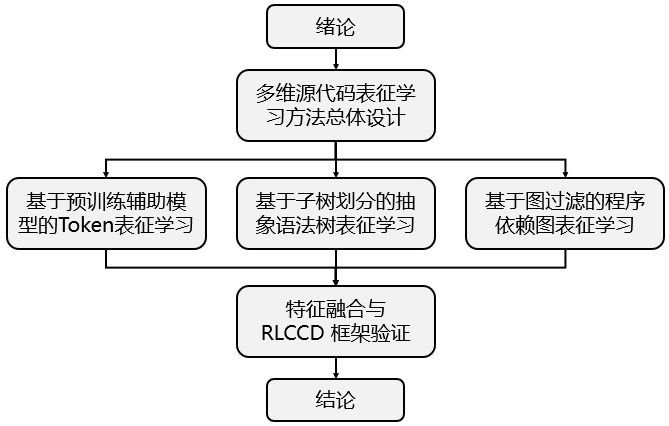
\includegraphics[width=0.85\textwidth]{figures/Structure}
    \caption{论文组织结构}\label{fig:Structure}
\end{figure}

\textbf{第1章} \quad 绪论部分首先对本文的研究背景与意义进行了阐述,之后对代码克隆检测技术和代码表征学习技术的研究现状与趋势进行了分析总结,进而提出本文的主要研究内容,最后介绍了全文的组织结构。

\textbf{第2章}  \quad 分析了代码表征学习领域的关键技术挑战,基于此,提出了本文的面向代码克隆检测的多维源代码表征学习方法RLCCD,并对该技术的整体框架进行了介绍,进而根据所提框架简要论述了本文研究的关键技术,即基于预训练辅助模型的Token表征学习方法、基于子树划分的抽象语法树表征学习方法、基于图过滤的程序依赖图表征学习方法,最后进行本章小结。

\textbf{第3章}  \quad 介绍基于预训练辅助模型的Token表征学习方法的设计与实现。首先,分析其研究动机,即目前Token表征学习面临的集外词问题,继而提出基于预训练辅助模型的方法设计,详细介绍该方法的设计思路和具体实现,最后,通过消融实验验证,评估本章提出的预训练辅助模型的有效性。

\textbf{第4章}  \quad 介绍基于子树划分的抽象语法树表征学习方法设计与实现。首先,分析其研究动机,即目前抽象语法树表征学习面临的梯度消失问题,继而提出基于子树划分的方法设计,详细介绍该方法的设计思路和具体实现,最后,对该方法的有效性进行消融实验验证。

\textbf{第5章}  \quad 介绍基于图过滤的程序依赖图表征学习方法设计与实现。首先,分析其研究动机,即目前图表征学习面临的规模开销问题,继而提出基于图过滤机制的方法设计,详细介绍该方法的设计思路和具体实现,并给出了针对该方法有效性的消融实验验证。

\textbf{第6章}  \quad 介绍特征融合及本文研究框架RLCCD的实验验证。首先,针对特征融合的方法设计与具体实现进行了介绍。接着,对RLCCD框架的有效性进行了评估,通过与现有开源技术SourcererCC\cite{7886988}、ASTNN\cite{8812062}、SCDetector\cite{10.1145/3324884.3416562}进行实验对比,验证RLCCD方法的有效性。

\textbf{结论}  \quad 首先对全文的研究工作进行了总结,并讨论本文的主要贡献与创新之处,最后对下一步可开展的工作提出展望。
\chapter{多维源代码表征学习方法总体设计}
\label{chap:design}

本章首先阐述了当前代码表征学习面临的一些关键技术挑战,进而针对现有问题提出面向代码克隆检测的多维源代码表征方法RLCCD,然后就该框架的总体架构和处理流程进行详细阐述,最后给出了下游代码克隆检测任务的问题定义,并针对RLCCD框架给出了形式化描述。

\section{代码表征学习面临的技术挑战}
\label{sec:challenges}
目前已有的代码克隆检测方法大多遵循以下思路:(1)首先对代码片段进行预处理;(2)对处理好的代码片段进行代码表征,将其转换为中间表征;(3)根据表征方式的不同计算不同代码片段之间的相似度,完成克隆检测任务。在代码克隆检测中,源代码表征方式决定了信息抽取的程度和粒度,进而影响了后续克隆检测的精度和效率。如何得到丰富且有效的源代码表征表示,是解决代码克隆检测任务的关键所在。从目前多种维度的代码表征方法来看,现有的代码表征方式存在以下技术挑战:

(1)Token维度代码表征存在集外词问题

基于Token的方法一般会利用词法分析器将源代码中的词汇单元Token划分出来,得到Token序列,并过滤掉无用的空格、注释、字符等,然后利用深度学习技术对其进行建模,生成具有丰富代码信息的表征向量,应用于下游代码任务。这类方法和自然语言处理(NLP)领域中常用来处理文本的方式很相似,产生一个规模巨大且稀疏的词汇表。但是,在大多数基于Token的代码克隆检测工具中,通常会将词法单元规范化,例如:将变量名用统一的标识符来代替。经过规范化Token产生的词汇表较小,导致模型学习能力有限,并且在训练过程中会出现未见过或未包含在词汇表中的词语。这些词语可能是用户自定义词、拼写错误、缩写、专有名词等。由于模型在训练阶段没有足够的信息来学习这些词语的表示,因此在实际应用中无法正确处理这些词语,从而导致模型的性能下降,这就是集外词(Out of vocabulary,简称OOV)问题。集外词问题会对模型的性能和泛化能力造成影响,严重限制了代码表征的有效性。

(2)树维度代码表征存在梯度消失问题

基于树的方法将代码通过语法解析转换成相应的抽象语法树,从而有效地表示代码的语法及其结构信息。与自然语言处理领域的长文本类似,当上下文序列很长的时候,基于树的神经网络模型容易出现梯度消失的问题,即梯度在训练过程中变得越来越小,导致模型发散或者训练不收敛。目前大多数基于树的代码克隆检测方法为了简化或者提高效率,通常会将生成的抽象语法树转换为完整的二叉树,在转换过程中,不仅破坏了源代码原有的语法结构,也会增加树的高度,进一步削弱模型捕捉复杂语义的能力,导致检测性能下降。

(3)图维度代码表征存在规模和开销问题

基于图的方法会将源代码表征为数据流图或者控制流图\cite{刘嘉勇2022源代码漏洞静态分析技术},数据流图代表了源代码中数据的走向,控制流图代表了代码中语句执行时的跳转流向。大多数基于图的代码克隆检测工具任务的核心是将图中的每个节点映射到一个低维、稠密的特征向量中,并将这些特征编码为特征矩阵,这一步通常需要大量空间开销。同时子图匹配算法是NP完全问题,计算成本过长,时间复杂度很高,因此图维度代码表征学习会存在算法计算开销大,可扩展性不好,检测结果召回率低等问题。

(4)代码表征存在信息利用不充分问题

虽然目前代码表征在Token、树、图等多种维度的研究已经取得了一定的进展,但仍存在信息利用不充分的问题。代码不仅仅具有文本自然性,同时具有结构信息、语义信息,但在现有的表征粒度中,Token维度的代码表征通常只关注文本自然性,抽象语法树缺乏对代码语义信息的捕捉,程序依赖图存在冗余信息,因此只使用单个特征来表示代码是远远不够的,很难覆盖所有信息,存在信息利用不充分,特征表达不完善的问题。

\section{RLCCD研究方案}
\label{sec:Framework}

\subsection{研究思路及总体框架}
\label{subsec:Ideas}
针对\ref{sec:challenges}节提出的四个技术挑战,本文提出了如图\ref{fig:thinking}所示的研究思路。

具体地,本文主要针对代码表征学习的三个维度展开研究工作:(1) 针对Token序列特征挖掘,提出预训练增强辅助模型提取属性特征,从而解决传统基于Token序列的方法存在的集外词问题;(2)针对抽象语法树AST特征挖掘,提出子树划分的改进方法提取结构特征,从而解决传统基于抽象语法树的方法存在的梯度消失问题;(3)针对程序依赖图PDG特征挖掘,提出过滤机制提取语义特征,通过收集PDG的简单特征来过滤输入神经网络模型的输入,从而解决传统基于程序依赖图的方法存在的规模开销问题。

同时,考虑到经由不同表征方式处理所得到的信息通常具有互补性,且不同维度的特征都是代码表示的平行语料,具有信息等价性,因此,本文提出基于多模态学习的特征融合方法,通过融合多个代码特征,包括非结构化(顺序Token形式的代码)和结构化(抽象语法树和程序依赖图形式的代码)信息,从多维数据中学到更好的特征表示,从而提高下游代码克隆检测任务的检测精度。

\begin{figure}[htp]
    \centering
    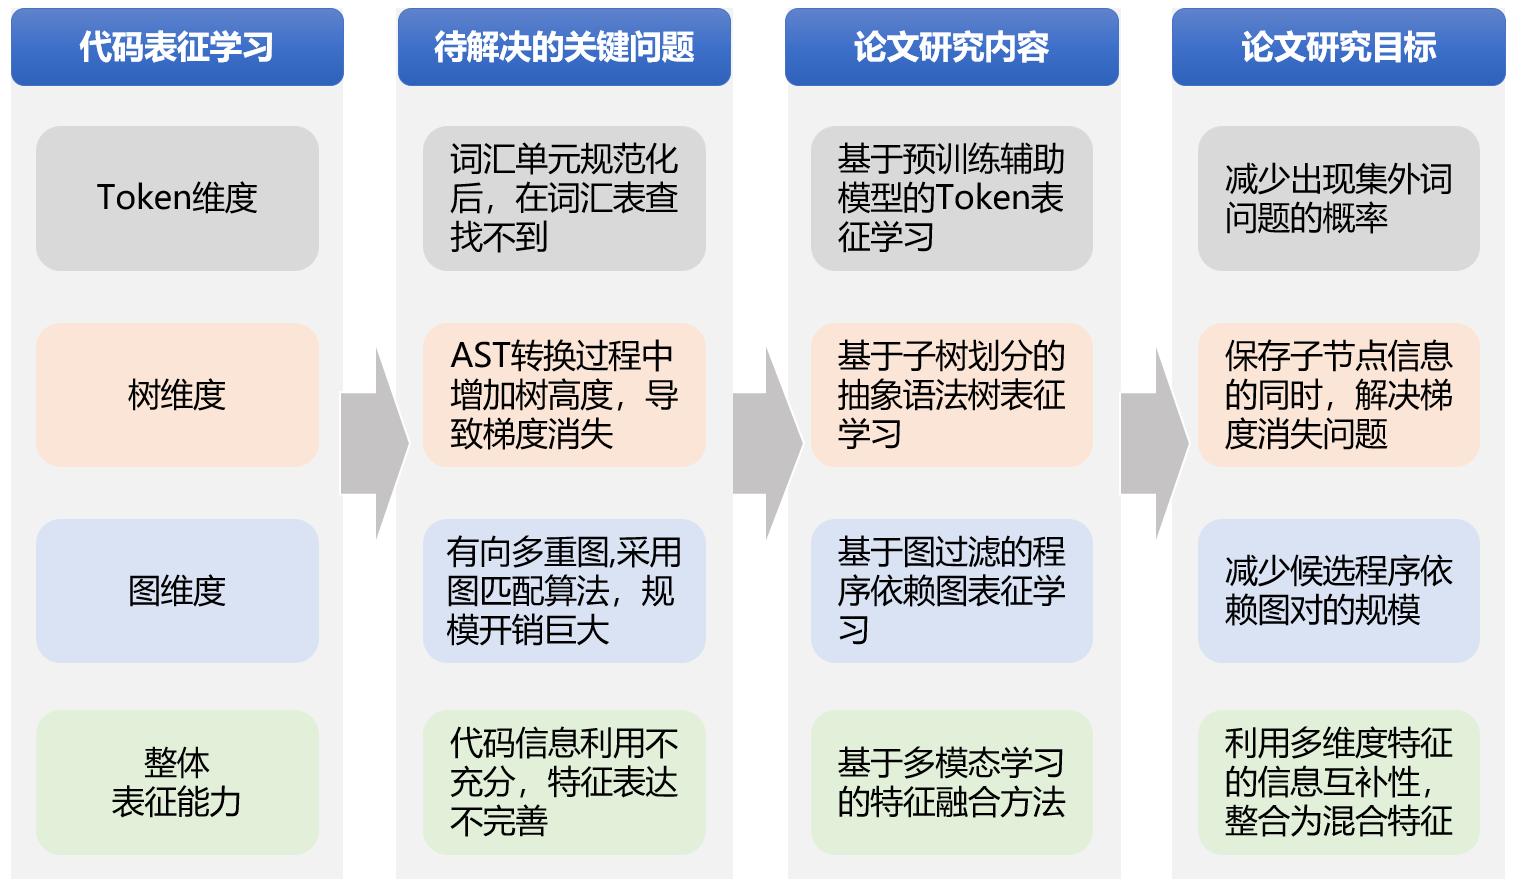
\includegraphics[width=0.75\textwidth]{figures/thinking}
    \caption{研究思路}
    \label{fig:thinking}
\end{figure}

本文基于上述研究思路,设计了面向代码克隆检测的多维源代码表征方法RLCCD,框架如图\ref{fig:framework}所示。由图\ref{fig:framework}可见,本文提出的基本框架与\ref{subsec:Code clone detection}节提出的代码克隆检测的处理流程基本一致,并主要通过三个维度对代码表征学习环节进行改进,然后对三个维度得到的特征向量进行特征融合,得到的混合特征应用到下游代码克隆检测任务中。

\begin{figure}[htp]
    \centering
    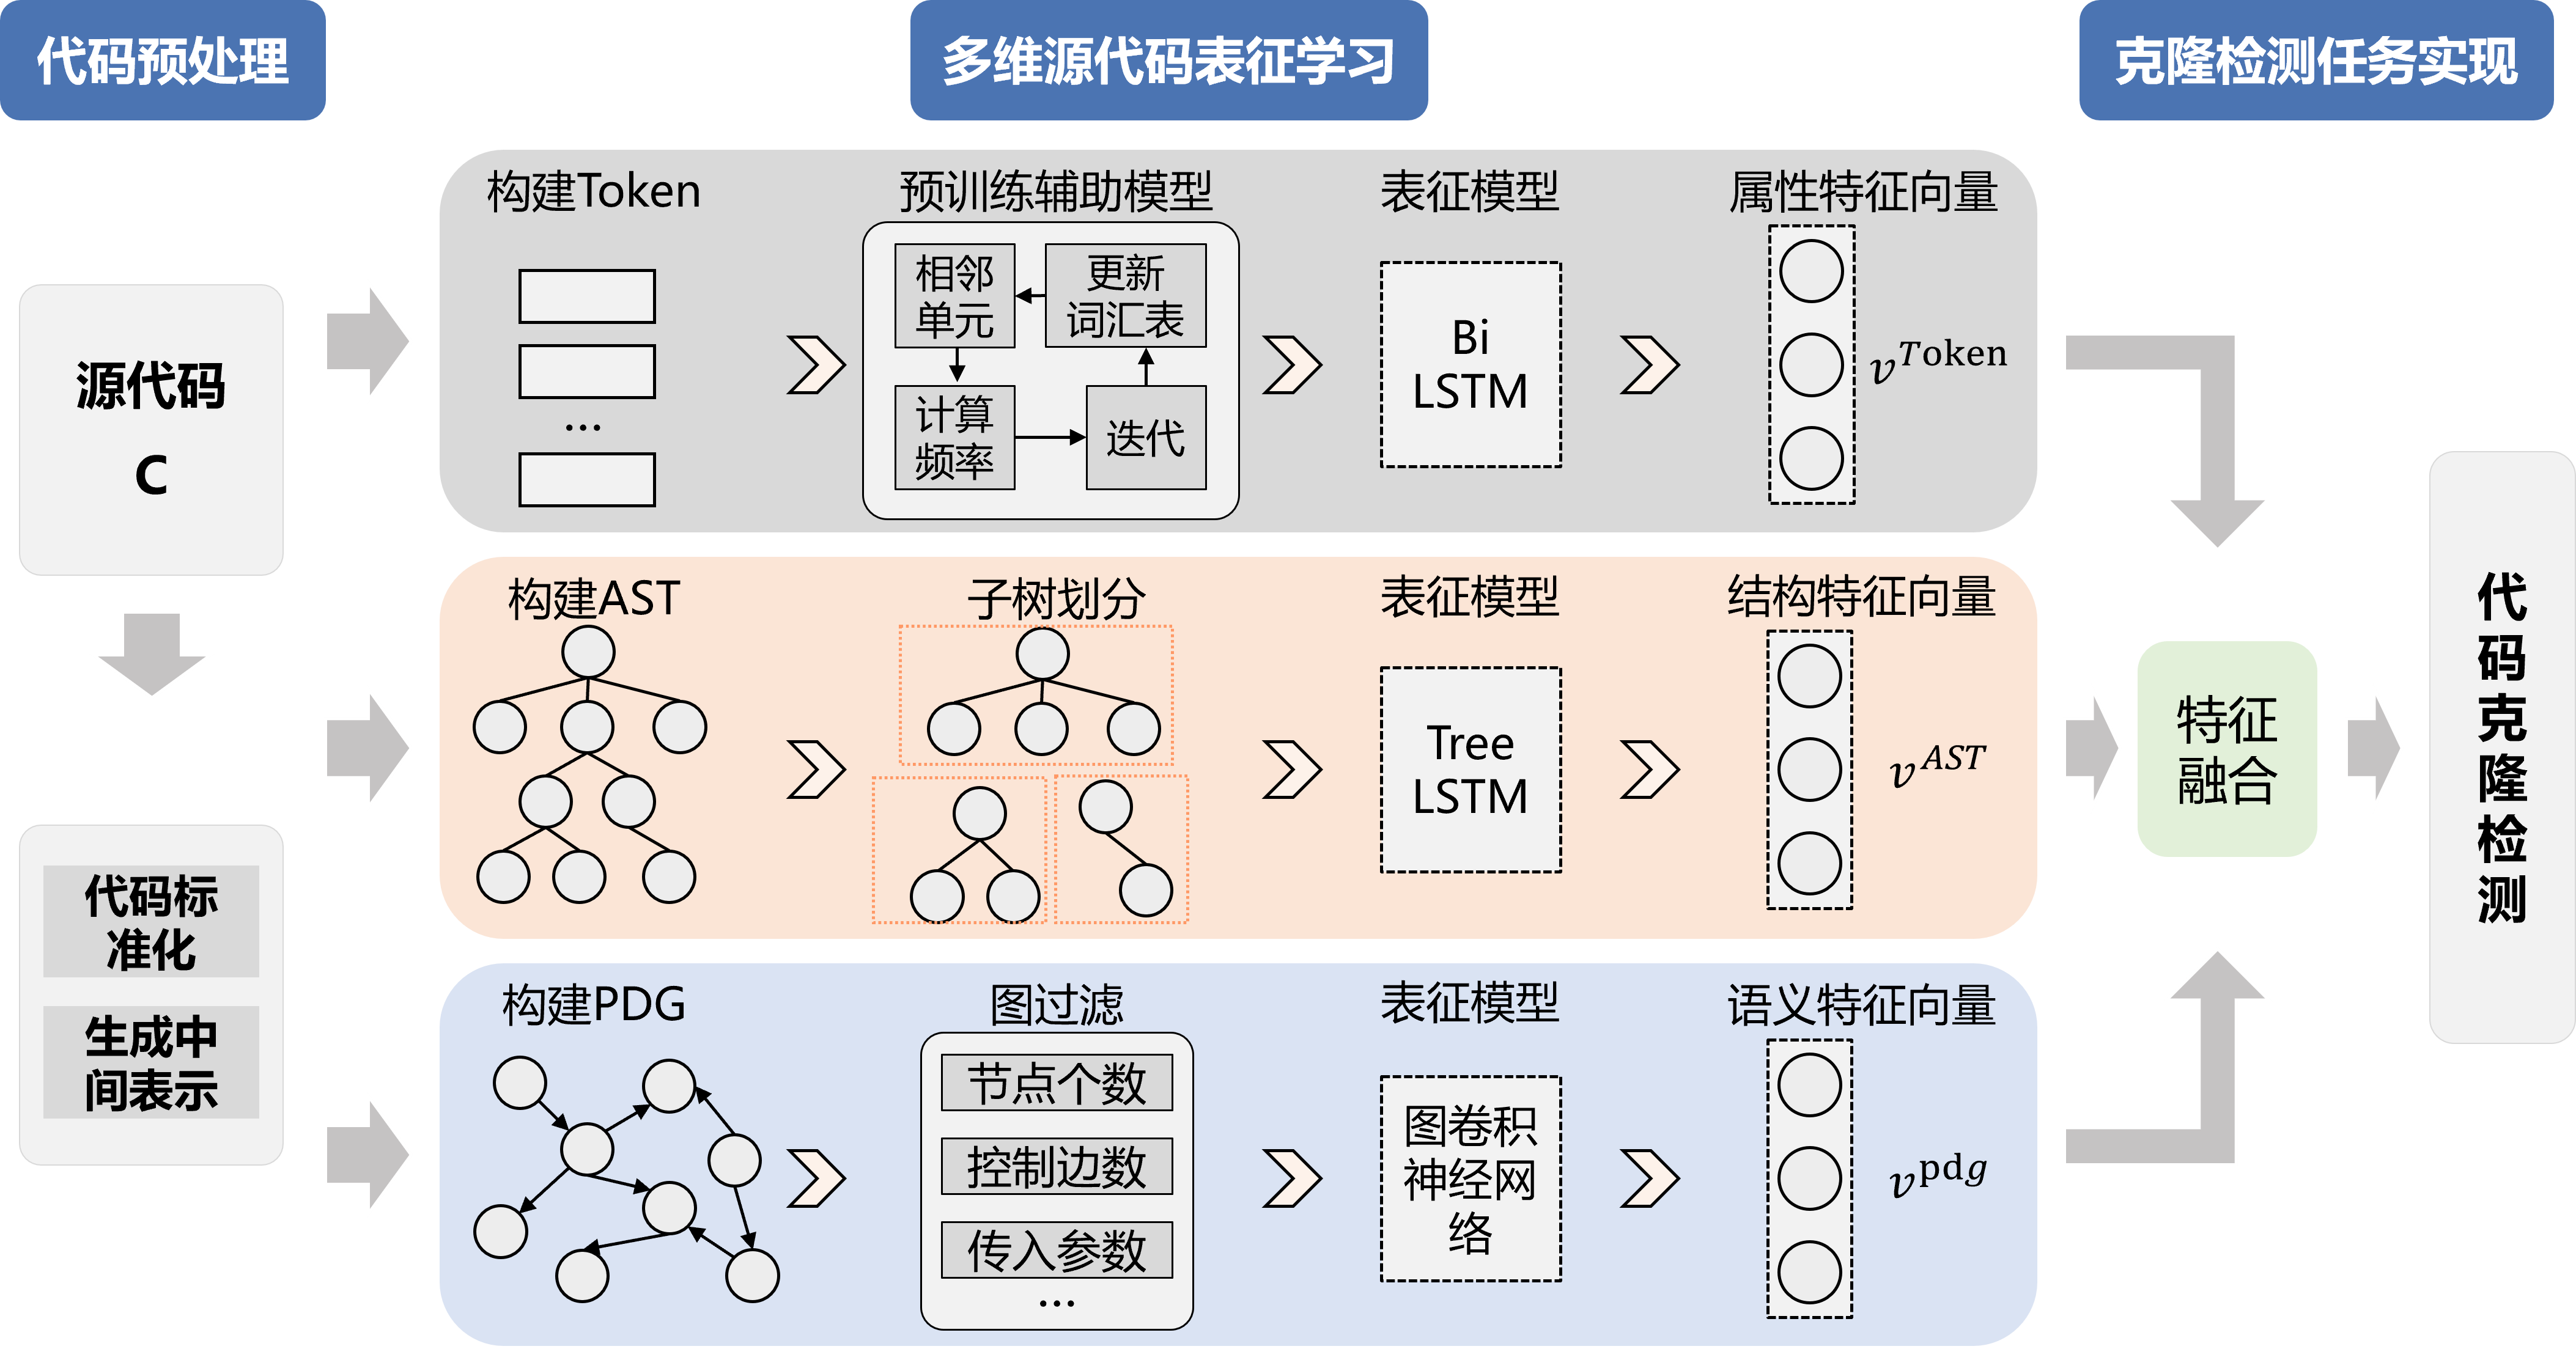
\includegraphics[width=0.75\textwidth]{figures/framework}
    \caption{RLCCD 总体框架}
    \label{fig:framework}
\end{figure}

\subsection{代码预处理}
\label{subsec:Preprocess}
代码预处理的目标是生成源代码片段对应的词法单元Token序列、抽象语法树AST和程序依赖图PDG,主要包含2个流程:代码标准化、生成中间表示。

(1)代码标准化

代码标准化的任务是去除与源代码无关的信息。首先是删除源代码片段中的注释、空行以及特殊符号,包括单行注释、多行注释、引入标准库的宏符号“\#”、无关符号等。其次,由于代码本身是一段包含丰富信息的文本,开发者通常会通过个人命名习惯对常量等标识符进行命名,这些私人信息并没有太多实际意义,反而会降低后续代码处理的精确率。因此,本文定义了转换规则,将代码中的某些标识符转换为对应的标记,在最大限度地保留原有重要信息的同时,减少对关键语义联系的缺失。

(2)生成中间表示

基于标准化后的代码片段生成对应的中间表示:Token序列、抽象语法树AST和程序依赖图PDG。其中,词法单元Token序列可以通过词法分析器得到,词法分析器能够按照预定的语法规则将代码中的字符串分割为一个个词汇单元,这些词汇单元包含代码标准化处理后的标识符;抽象语法树AST以树状的形式抽象描述了程序语句的语法结构信息,生成抽象语法树时需要对源代码文本进行词法分析,然后依据语法规则分析整合Token,得到树型结构;程序依赖图PDG能够表示源代码的控制依赖,数据依赖等关系,是一种带有标记的有向多重图。生成程序依赖图时,需要对程序进行语法分析,然后分析程序中变量的关联关系,根据这种关联关系描绘程序的数据依赖和控制依赖关系,形成图的描述。

\subsection{多维源代码表征学习}
\label{subsec:Representation}
RLCCD框架的核心步骤是源代码表征学习,其目标是学习能够表示代码片段的连续向量,表现程序理解的认知层次,获取程序的语法、语义信息,创建程序更高抽象层次上的表示;它决定着对源代码信息抽取程度的上限,决定着检测方法的预处理方式、模型设计、部署方式、运行效率,并影响后续代码克隆检测任务所能检测的精度。本文提出的多维源代码表征学习方法包括Token序列、抽象语法树AST、程序依赖图PDG三种不同维度,并分别对其进行了优化改进。

(1)词法单元Token

传统的基于Token的表征学习方法通常将代码表示为词汇单元,为了后续生成表征向量通常会将词汇单元规范化,导致丢失部分语法信息,出现在词汇表中不存在Token的难题。针对这样的问题,本文提出了一种预训练辅助模型的改进方法提取属性特征。具体来说,通过选取预训练辅助模型从代码语料库中学习基本单元的语法语义信息,以及这些单元之间的联系,最终给出一份单词-向量形式的词汇表,从而减少出现集外词问题的概率。

(2)抽象语法树AST

抽象语法树中包含了代码片段的结构信息,然而,传统的基于树的代码表征学习方法通常将抽象语法树转换为完整二叉树,可能破坏源代码原有的语法结构,增加AST高度,丢失长期上下文信息,削弱了神经网络模型捕捉更真实和复杂语义的能力,导致梯度消失的难题。针对这样的问题,本文提出基于子树划分的改进方法提取结构特征。具体来说,将每个大型的抽象语法树分解为小语句树序列,并通过捕获语句的词法和句法知识将每一个语句树都编码成一个向量。在得到一个语句向量序列后,将语句向量序列输入网络中生成代码片段的结构向量表示。这种细粒度的处理使得模型可以很好地处理很深的抽象语法树,解决梯度消失问题。

(3)程序依赖图PDG

程序依赖图中包含代码片段的控制依赖,数据依赖赖等语义关系,然而,传统的基于图的代码表征学习方法通常采用图匹配算法将图中的控制流和数据流编码为一个紧凑的语义特征矩阵,且矩阵中每个元素都是高维系数特征向量,面临消耗的时间、空间开销巨大的难题。针对这样的问题,本文提出了基于图过滤机制的改进方法提取语义特征。具体来说,根据PDG的节点个数、控制边数、执行边数、数据边数、声明节点数、函数调用数、传入参数、传出参数等典型特征进行过滤,减少模型的输入规模。

(4)特征融合方法

特征融合的目标是将提取到的属性特性、结构特征、语义特征合并,得到一个更能代表代码信息的多维特征。具体来说,通过三个不同维度得到属性特性、结构特征、语义特征,然后使用特征连接Concat、特征加法Add两种融合方式将三个特征映射到相同的特征空间内,得到一个多维表征,包括非结构化(顺序Token形式的代码)和结构化(抽象语法树和程序依赖图形式的代码)信息。该多维特征能够在低维空间中高效计算实体和关系的语义联系,挖掘代码更全面、层次更深的信息,从而提高后续下游的代码克隆检测任务的准确率。

\subsection{克隆检测任务实现}
\label{subsec:Clone detection}
克隆检测任务实现的核心任务是判断两个代码片段是否是真克隆对。经过\ref{subsec:Preprocess}节代码预处理和\ref{subsec:Representation}节多维源代码表征学习两个步骤,可以得到对应的多维特征向量表示作为输入,然后计算这两个向量之间的相似性判断是否存在代码克隆。目前,常见的计算向量相似性的方法包括计算距离度量\cite{FRENKLACH2021102386}、相似性度量\cite{Mallik2022ConRecMC}两种,向量的距离越近相似度越大。一些研究倾向于把程序表征为向量形式,使用余弦相似度、Jaccard相似度、欧几里得距离、汉明距离、曼哈顿距离等评估指标计算向量之间的相似度,当相似度大于某个固定阈值时则认为存在代码克隆。具体的,本文通过将待测代码克隆对的多维特征向量输入分类模型,计算其向量距离,并定义二元交叉熵为损失函数,以最小化损失为目标训练分类模型,完成代码克隆检测任务。

\section{RLCCD定义描述}
\label{sec:RLCCD flow}

本节给出面向代码克隆检测的多维源代码表征学习方法RLCCD的数学化定义描述。给定两个代码片段$C_{a},C_{b}$,使用一个三元组$(C_{a},C_{b},y_{ab})$形式来表示一对代码片段,其中$y_{ab}$表示标签。如果$(C_{a},C_{b})$是一个克隆对,那么$y_{ab}$为1,否则$y_{ab}$为0。从$n$个代码片段中构建一个带有标签的训练集$\left\{(C_{a},C_{b},y_{ab})|a,b \in n,a<b\right\}$,本文的目的是训练一个深度学习模型来学习一个可以把代码$C$映射成一个特征向量$V$的函数$f$。对于任意代码片段对,通过函数$f$得到一对特征向量,然后计算出它们的相似度分数$S_{ab} = Sim(f(C_{a}),f(C_{b}))$并进行分类,使其分类结果尽可能接近已知的标签$y_{ab}$。在预测阶段,为了推断出两个代码片段是否是克隆对,在真假克隆对之间设置了一个阈值$k$,如果预测的相似度分数大于$k$值,那么认为两个代码片段是真克隆对,否则,认为它们是假克隆对。其中,训练一个深度学习模型将代码$C$映射成一个特征向量$V$的过程,可以视为代码表征学习的数值化过程,也是本文研究的重点。

面向代码克隆检测的多维源代码表征学习方法RLCCD流程如图\ref{fig:flow}所示,采用Siamese架构。RLCCD方法的输入是两个代码片段$C_{a},C_{b}$,输出是一个0或1的标签,1表示这两个代码片段是真克隆对,0表示是假克隆对。Siamese架构采用两个不同的输入,通过两个具有共享权值的相似子网络,输出一个标签来计算两个输入之间的相似度。整个方法的执行包括四个步骤,分别是:
\begin{figure}[htp]
    \centering
    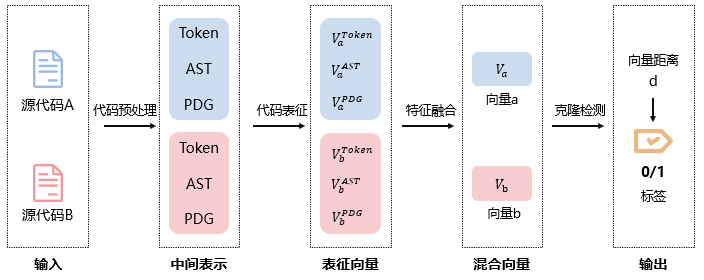
\includegraphics[width=0.95\textwidth]{figures/flow}
    \caption{面向代码克隆检测的多维源代码表征学习方法RLCCD流程图}
    \label{fig:flow}
\end{figure}

\textbf{代码预处理}:RLCCD接受两个代码片段$C_{a},C_{b}$作为输入,通过代码预处理阶段,得到对应的中间表示:词法单元Token序列、抽象语法树AST、程序依赖图PDG。

\textbf{代码表征}:代码表征是本文的核心步骤,输入是代码片段$C_{a},C_{b}$对应的中间表示,输出是对应的表征向量,分别记为代码片段$C_{a}$的属性特征$V_{a}^{Token}$、结构特征$V_{a}^{AST}$、语义特征$V_{a}^{PDG}$,代码片段$C_{b}$的属性特征$V_{b}^{Token}$、结构特征$V_{b}^{AST}$、语义特征$V_{b}^{PDG}$。

\textbf{特征融合}:特征融合阶段的输入是代码片段$C_{a},C_{b}$的特征向量,输出是对应的混合向量$V_{a},V_{b}$。本文将提取到的属性特性、结构特征、语义特征合并,得到一个更能代表代码信息的多维特征。用公式\ref{e2.1}表示特征融合。

\begin{equation}\label{e2.1}
    \mathrm{V}= v^{\text{Token}} \bullet v^{\text{AST}} \bullet v^{\text{PDG}}
\end{equation}

其中$\bullet$表示特征融合方法,$V$表示最终的多维混合代码表示。

\textbf{克隆检测}:经过三个步骤,可以得到代码片段对应的向量表示$V_{a},V_{b}$。由于代码克隆检测问题是一个二分类问题,即给定两个代码片段,需要输出0或1,0表示它们之间不相似,1表示相似。因此通过公式\ref{e2.2}计算代码片段$C_{a}$对应的多维表征$V_{a}$与代码片段$C_{b}$对应的多维表征$V_{b}$之间的距离$d$,并将向量距离$d$映射到0$\sim$1之间,将输出值作为两个代码片段的相似度$S_{ab}$。
\begin{equation}\label{e2.2}
    \begin{split}
    d &= \left|V_{a}-V_{b}\right| \\
    \mathrm{S_{ab}} &=\operatorname{sigmoid}\left(d\right) \in[0,1]
    \end{split}
\end{equation}

并将损失函数定义为二元交叉熵,如公式\ref{e2.3}所示,训练模型的目标是最小化损失。
\begin{equation}\label{e2.3}
    J(\Theta, S_{ab}, y_{ab})=\sum(-(y_{ab} \cdot \log (S_{ab})+(1-y_{ab}) \cdot \log (1-S_{ab})))
\end{equation}

其中,$y_{ab}$表示两个代码片段的真实标签。

当所有参数都设置为最优化后,模型被存储起来。在预测阶段,通过公式\ref{e2.4}得到预测值。
\begin{equation}\label{e2.4}
    \text { prediction }=\left\{\begin{array}{ll}
        1, & S_{ab}>k \\
        0, & S_{ab} \leq k
        \end{array},\right.
\end{equation}

\section{本章小结}
\label{sec:Summary2}
本章首先给出了代码克隆检测问题的定义,然后分析了源代码表征学习在代码克隆检测过程中所面临的关键技术挑战,主要表现为Token集外词问题、树梯度消失问题、图规模开销、单个表征维度对代码信息利用率低问题。针对四个问题,本文提出了面向代码克隆检测的多维源代码表征学习方法RLCCD,在介绍了其整体框架后,对其中的关键技术点进行了简要的论述,最后详细描述了RLCCD的处理流程。

\chapter{基于预训练辅助模型的Token表征学习}
\label{chap:Token}
本章主要对本文提出的基于预训练辅助模型的Token表征学习方法进行详细介绍,首先介绍其研究动机,接着阐述其方法设计,以及具体的实现过程,最后介绍实验验证过程和结果。

\section{研究动机}
\label{sec:Motivation}

基于Token的代码表征方法本质上就是将源代码转换为一系列词法单元Token组成的序列,并对Token序列进行代码分析。类似于自然语言技术处理文本,由于源代码中存在大量用户自己定义的标识符,不同用户的命名习惯不同,在对源代码的词法单元建模时,会产生一个规模巨大且稀疏的词汇表。该词汇表的规模会直接影响代码分析任务的效率,因此现有方法大多都对Token进行规范化,比如将变量名用统一的标识符来代替,从而降低词汇表的规模。但是后续神经网络模型训练过程中,当出现某个词汇在词汇表中没有出现过,那么神经网络模型就无法对齐建模,即出现了在词汇表中不存在的Token,集外词(Out-of-vocabulary,简称OOV)问题。有研究\cite{RJXB202205011}发现,针对代码表征中的集外词问题,在经典BigcloneBench\cite{7332459}数据集中OOV比率高达62.68\%,在OJClone数据集\cite{WOS:000485474201046}中OOV比率达到了16.82\%。

为了解决OOV问题,本文打算使用预训练模型增加词汇表的大小。近期,研究人员在大规模语料库上预训练各种语言模型,在解决各种自然语言处理任务方面取得了良好进展\cite{zhao2023survey}。在表征学习领域,也有基于大规模预训练模型提升代码表征能力的方法被提出。InferCode\cite{9402028}将自然语言处理中的自监督学习思想引入到代码的抽象语法树的表示中, 通过预测从AST上下文中自动识别的子树来训练代码表征,并且使用AST的子树作为训练标签,从而无需任何人工标记工作。该预训练InferCode模型可以应用于下游的无监督学习,例如代码聚类、代码克隆检测、跨语言代码搜索等。GraphCodeBERT\cite{guo2021graphcodebert}方法提出了一个基于数据流的代码表征预训练模型,与抽象语法树不同,数据流包含代码变量间“值从哪里来”的语义特征,并不会带来深层次不必要的复杂信息,使用该特征可以更有效的生成代码表征。然而这些预训练模型通常存在参数规模庞大, 训练及使用代价大的问题。

因此,针对集外词OOV问题,本文提出了一种轻量级的基于预训练辅助模型的Token表征学习方法,该方法在提升代码表征能力的同时,并不会引入过多参数,造成模型训练代价高的问题。

\section{Token表征方法设计}
\label{sec:Token}
本节将主要介绍基于预训练辅助模型的Token表征学习方法的详细设计,首先介绍该方法的整体框架,并分别从预训练辅助词嵌入、Token代码表征两方面介绍具体设计。

\subsection{框架概述}
\label{subsec:TokenOverview}
本文提出的基于预训练辅助模型的Token表征学习方法的整体框架如图\ref{fig:tokenframework}所示。该框架的输入是代码片段对应的Token序列,输出是对应的属性特征向量,主要包括预训练辅助词嵌入、Token代码表征两个阶段。

\begin{figure}[H]
  \centering
  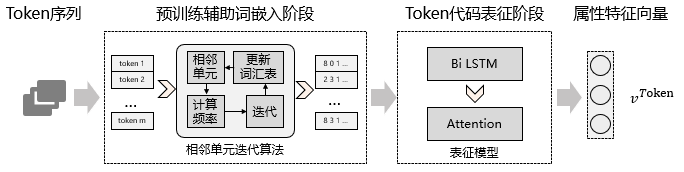
\includegraphics[width=0.95\textwidth]{figures/tokenframework}
  \caption{基于预训练辅助模型的Token表征学习框架}\label{fig:tokenframework}
\end{figure}

首先,预训练辅助词嵌入阶段以代码片段的Token序列作为训练数据,构建一个预训练辅助词嵌入模型。该模型的输入是代码片段对应的Token序列,输出为与输入对应的Token词嵌入向量。然后通过对模型的训练,使得该模型具有正确识别Token的能力,并将该模型保存下来。需要注意的是,为了减少集外词OOV问题,本文对模型采用相邻单元迭代算法,即,通过多次迭代来更新词汇表。

其次,Token代码表征阶段以Token词嵌入向量作为训练数据,构建一个Token表征模型。该模型的输入是Token序列对应的词向量,输出为一个固定长度的密集向量用来表示代码的属性特征。需要注意的是,本文选用的AttBiLSTM神经网络,主要包含两个部分:双向长短时记忆部分(BiLSTM)和自注意力机制部分(Attention),前者主要目的是同时捕获序列的双向语义信息,后者的主要目的是总结序列的输入特征,并将每个代码片段缩减为一个单一的密集向量。

在上述框架中,本文的创新点主要体现在预训练辅助词嵌入阶段的相邻单元迭代算法、Token代码表征阶段的模型设计两方面,下面将围绕这两个创新点来阐述本文的方法。

\subsection{预训练辅助词嵌入设计}
\label{subsec:Model}

与自然语言处理类似,源代码的词法单元Token可以视为句子中的单词,Token维度的代码表征方法第一步就是将词法单元Token转换为机器易于理解和操作的数值向量,即词嵌入技术。它将词汇表中的每个单词转换成一个低维度、连续的向量表示,这种向量通常被称为词向量。目前,使用预训练词嵌入模型训练词向量的研究工作发展迅速,Word2vec、GloVe、FastText、ELMo和BERT等模型也相继被提出。其中,Word2vec模型通过从大规模无标注文本数据集中学习上下文信息,自动捕捉并编码词汇的语义关系,生成的词嵌入向量作为下游任务的输入特征,可以显著提升神经网络模型的性能和泛化能力。因此,本文采用Word2vec模型进行词嵌入。

同时,为了减少集外词OOV问题出现的概率,本文提出了一种相邻单元迭代算法(Adjacent token iterative algorithm,ATIA),该算法通过组合Token序列中相邻单元构造新的代码表示单元,然后统计新单元出现的频率,根据频率信息多次迭代,不断更新词汇表。下面对相邻单元迭代算法进行介绍。

具体的,首先将代码数据集中的源代码经过代码预处理,得到对应的Token序列作为初始语料库。然后按照代码块组合相邻Token并查找出出现次数最频繁的Token组合,并将这个组合称为新的迭代单元Adjacent gram,简称Agram。最后将这个Agram当作新的独立单元,加入到词汇表中,而原本组成这个Agram的原始Token单元并不会从词汇表中删除。在第一次迭代的时候,选取相邻的两两Token作为组合,把出现最频繁的Token组合确定为一个Agram单元之后再进行二次迭代,每次迭代在原来的基本单元上再组合一个新的邻近Token作为新的判断单元,不断的进行迭代,每次迭代都要对应的更新词汇表。

相邻单元迭代算法ATIA的伪代码如\ref{alg1}所示。该算法有两个输入:待处理的初始Token语料库、迭代次数,输出为经过多次迭代后生成的语料库,具体包括初始化AgramsSet、计算单元Agram出现的次数、更新语料库3个步骤,具体来说,每个步骤的作用如下:

\begin{algorithm}[ht!]  %ht!参数是调整算法在文章中的位置
	\renewcommand{\algorithmicrequire}{\textbf{Input:}}
	\renewcommand{\algorithmicensure}{\textbf{Output:}}
	\caption{Iterative algorithm main function}  
	\label{alg1}
	\begin{algorithmic}[1]
    \Require Tokens Corpus $Corpus$
    \Require The number of iterations $N$
		\Ensure New Corpus $NewCorpus$
    \State $AgramsSet = \varnothing $ \Comment{step1:初始化AgramsSet} 
		\For{$int i \leftarrow 1 to N$}
      \If {i == 1}
        \State $ AgramSet \leftarrow set([token for tken in line for line in sentence])$
      \Else
      \State $Atokens(A_i) = learn_algorithm(Token(T_i)) $ \Comment{调用learn算法获取当前一轮的迭代结果,更新Agrams数组}
      \State $Agram = max(Agrams) $ \Comment{计算单元Agram出现的次数}
      \State $ add Agram to Vocab(V_i)$ \Comment{更新语料库}
      \EndIf
    \EndFor \\
    \Return $NewCorpus = [vocab[line] for line in sentences]$
	\end{algorithmic}
\end{algorithm}

(1)初始化AgramsSet

该算法的主要作用是控制算法逻辑,调用其他方法。在算法的第一行大的For循环里控制迭代的次数,每次迭代都需要调用Funtion 2进行具体的处理,获取到Funtion 2返回的的结果,即当前迭代轮次得到的所有Token组合和对应的出现次数(算法第二行),再根据次数选取出出现次数最多的组合(算法第三行),将这个新的组合作为一个新的单元Agram,调用Funtion 3把这个新的单元添加到语料库中(算法第五行)。第一次迭代,组合相邻Token,得到Agram组合并计算这些组合在语料库中出现的次数。首先要初始化一个词典用来存放最终结果(算法第一行),在具体组合过程中,首先把代码按照语句也就是行进行
分割(算法第二行),然后把这个语句切割为oken 存入一个集合(第三行)。依次遍历这些集合通过组合相邻的token获取新的基本单元(算法第四、五行),

(2)计算单元Agram出现的次数 

时遍历语料库获取这些组合在语料库中出现的次数。最后把 token 组合当作 key,组合出现的次数当作对应 key 的 value 值返回给调用函数。

(3)更新语料库

% 如果原始语料库中存在新的 bigram 单元就将该 bigram 单元放入语料库。接收的输入是当前最新的
% 语料库和主函数中确定的待合并的 token 组合 bigram。首先初始化一个空的语料库 new_corpus 用来存放新的语料(算法第一行),在最外层的 for 循环中进行和算法2第二行类似的操作,即将当前语句 statement 切割为独立的 token 存入集合。然后在一个 while循环中遍历集合(算法第四行),如果 segments 集合里第 i 个token 和第 i + 1 个 token 的组合等于传参给函数的 bigram(算法第五行),将第 i个 token 和第 i + 1 个 token 的组合 bigram 放入语料库 new_corpus(算法第六行)。如果不满足 if 判断,就直接把第 i 个 token 存入 new_corpus,继续循环判断。这样就可以保证即使某个 token 不存在于任何一个 bigram 单元,该 token 也会以一个单独的单元存放于语料库中。最后将合并之后最新的语料库 new_corpus 返回给主函数。


\subsection{Token代码表征设计}
\label{subsec:Token}

将token序列对应的向量输入到Bi LSTM网络中,经过Bi LSTM学习哪些信息应该被记住哪些信息应该被遗忘,最终得到每个基本单元包含语义信息和上下文信息的向量表示。Bi LSTM由一个正向的LSTM和一个反向的LSTM组成,主要思想是通过把序列向前、向后分别输入给两个独立的递归网络,这两个子网络连接到一个输出层,在每个词的输出部分把两个子网络的输出信息进行整合,这样网络就同时拥有了序列中每个词的过去时刻信息和未来时刻信息。Bi LSTM可以捕获到序列前后的关系依赖,将代码片段的Token序列转换为可相互比较的向量。

\section{Token表征方法具体实现}
\label{sec:achieve}
本文提出的基于预训练辅助模型的Token表征学习方法的实现如图\ref{fig:token}所示。该方法的输入是代码片段$C_{a},C_{b}$对应的Token序列,输出是$C_{a},C_{b}$对应的属性特征向量,整体采用Siamese架构,两个子网络共享权值。该框架主要包括预训练辅助词嵌入、Token代码表征两个阶段。

\begin{figure}[H]
  \centering
  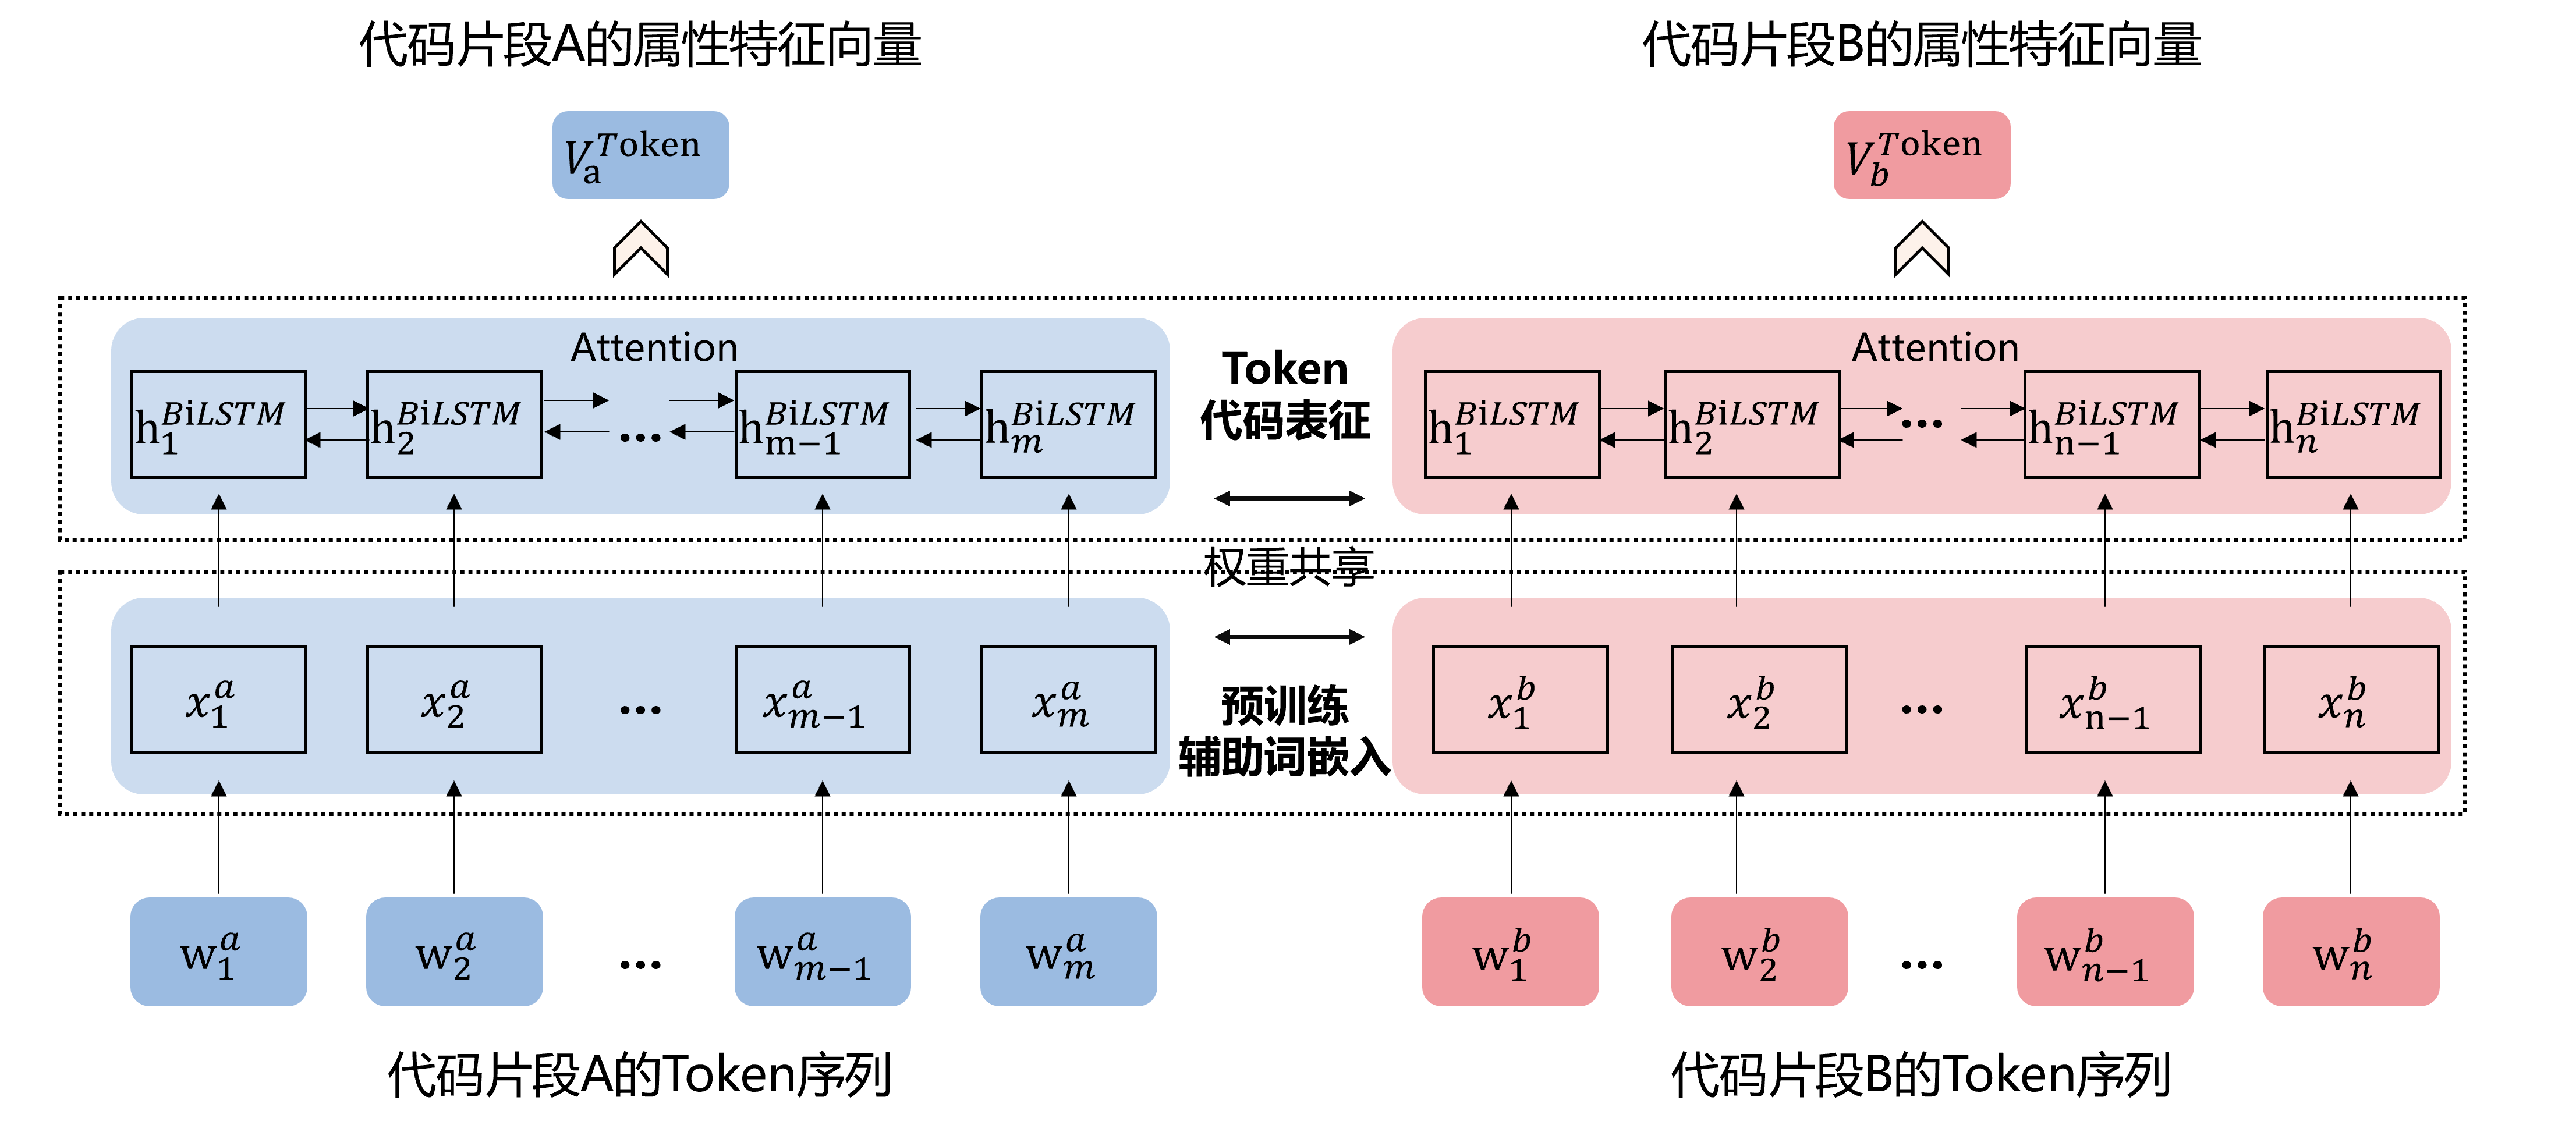
\includegraphics[width=0.95\textwidth]{figures/token}
  \caption{基于预训练辅助模型的Token表征学习方法实现}\label{fig:token}
\end{figure}


\section{实验验证}
\label{sec:Experiment}
为了验证基于预训练辅助模型的Token表征方法的有效性,本节展开实验验证。首先,介绍了实验整体的环境配置、数据集,以及实验评估;接着,对基于预训练模型的Token表征方法进行了消融实验。

\subsection{实验环境}
\label{subsec:Environment}
本章的实验验证均运行于Linux系统下,其系统硬件配置如表\ref{tab:environment}所示。

\begin{table}[H]
  \centering
  \caption{实验环境配置} 
  \label{tab:environment}
  \begin{tabular*}{0.6\textwidth}{@{\extracolsep{\fill}}cc}
  \toprule
    环境			&配置		\\
  \midrule
    操作系统		&Ubuntu 20.04 \\
    处理器			&Intel Core i9-12900KF × 24 \\
    内存			  &31.1G \\
    显卡			  &NVIDIA  \\
    磁盘			  &1TB \\
  \bottomrule
  \end{tabular*}
\end{table}

\subsection{实验数据集}
\label{subsec:Dataset}
为了验证预训练辅助模型在Token层面上表征学习的有效性,本文面向代码克隆检测任务对预训练辅助模型进行分析和评估,选取的实验数据为POJ104数据集。如表\ref{tab:dataset}所示,POJ104数据集是一个基于C语言所构建的大型数据集。OJ系统是一个以编程教学为目的公开评判系统,共存在104个编程问题,针对每个编程问题,学生们通过在线提交自己的代码来尝试解决,同时OJ系统将自动判断提交源代码的正确性和有效性。对于OJ系统中同一个编程问题来说,其所有正确提交的代码都为克隆代码,对于不同的编程问题所提交的代码,即为非克隆代码。POJ104数据集针对每一个编程问题,均提供500个学生提交源代码,即共有52000个样本。

\begin{table}[H]
  \centering
  \caption{POJ104数据集} 
  \label{tab:dataset}
  \begin{tabular*}{0.6\textwidth}{@{\extracolsep{\fill}}cc}
  \toprule
    代码			&属性		\\
  \midrule
    Dataset			&POJ104数据集 \\
    Language    &C \\
    Program			&52000 \\
    Classes			&104 \\
    Max tokens			&8737 \\
    Avg tokens			&245 \\
  \bottomrule
  \end{tabular*}
\end{table}

得到POJ104数据集后,本文首先对数据集进行初步筛选,去掉其中包含乱码的样本,共得到51485个源代码样本。然后对源代码进行预处理,删除样本中包含的空白行和注释等多余代码,并将数据集保存到一个program.pkl文件中,program.pkl文件中一共包含51485行×3列的数据集,每一行数据代表一个源代码样本,第一列为源代码id,第二列保存源代码样本code,第三列为源代码的标签label,即属于哪一个编程问题。接着,本文随机两两组合同一标签label的源代码,组成5200个真克隆对,随机组合不同标签的源代码组成44800个假克隆对,一共给包含50000个克隆对,并将其保存到oj\_clone\_ids.pkl文件中,oj\_clone\_ids.pkl文件中一共包含50000行×3列的数据集,每一行数据代表一个克隆对样本,第一列为源代码id1,第二列为源代码id2,第三列为克隆对的标签label,真克隆对标签为1,假克隆对标签为0。最后,依据随机种子将数据集按照3:1:1划分为训练集、测试集、验证集,其中的正负样本数如下表\ref{tab:ClonePairs}所示。

\begin{table}[H]
  \centering
  \caption{本文预处理后的POJ104数据集正负样本数} 
  \label{tab:ClonePairs}
  \begin{tabular*}{0.8\textwidth}{@{\extracolsep{\fill}}cccc}
  \toprule
    数据集			&真克隆对		&假克隆对		&克隆对数 \\
  \midrule
    训练集train			&3162	  &26838		&30000 \\
    测试集test			&1022		&8978		  &10000 \\
    验证集dev			  &1016		&8984		  &10000 \\
    总计            &5200	  &44800	  &50000 \\
  \bottomrule
  \end{tabular*}
\end{table}

\subsection{评估指标}
\label{subsec:Index}
代码克隆检测问题是二分类问题,因此本文采用准确率(Accuracy)、精确率(Precision)、召回率(Recall)、F1值四个评估指标来度量实验结果,其中使用了混淆矩阵中的TP、FN、FP、TN,如表\ref{tab:ConfusionMatrix}所示。

\begin{table}[H]
  \centering
  \caption{分类问题的混淆矩阵} 
  \label{tab:ConfusionMatrix}
  \begin{tabular*}{0.7\textwidth}{@{\extracolsep{\fill}}ccc}
  \toprule
  \multirow{2}{*}{实际值} & \multicolumn{2}{c}{预测值} \\
  \multirow{2}{*}{} & 正样本(P) & 负样本(N) \\
  \midrule
    正样本(P)			&TP	  &FN		 \\
    负样本(N)			&FP		&TN		 \\
  \bottomrule
  \end{tabular*}
\end{table}

其中,混淆矩阵中的真阳性、假阳性、真阴性、假阴性代表的含义如下:

真阳性(True Positive, TP):样本实际为正样本,并且被模型预测为正样本,即实际上标记为真克隆对并且被检测出来为真克隆对的代码对。
 
假阳性(False Positive, FP):样本实际为负样本,但是被模型预测为正样本,即实际上标记为假克隆对但是被检测出来为真克隆对的代码对。
 
假阴性(False Negative, FN):样本实际为正样本,但是被模型预测为负样本,即实际上标记为真克隆对但是被检测出来为假克隆对的代码对。
 
真阴性(True Negative, TN):样本实际为负样本,并且被模型预测为负样本,即实际上标记为假克隆对并且被检测出来为假克隆对的代码对。

准确率(Accuracy)表示预测为正的样本中真实值为正的比率,计算公式如\ref{e5}所示:
\begin{equation}\label{e5}
  Accuracy = \frac{TP+TN}{TP+FN+FP+TN} 
\end{equation}

精确率(Precision)表示正确检测到的代码克隆数量占全部预测为代码克隆的比例,计算公式如\ref{e6}所示:
\begin{equation}\label{e6}
  Precision = \frac{TP}{TP+FP} 
\end{equation}

召回率(Recall)表示正确检测到的代码克隆数量占总体实际代码克隆数量的比例,计算公式如\ref{e7}所示:
\begin{equation}\label{e7}
  Recall = \frac{TP}{TP+FN} 
\end{equation}

精确率(Precision)和召回率(Recall)指标有时候会出现的矛盾的情况,这样就需要综合考虑两者的表现,最常见的方法就是F1,精确率和召回率的加权调和平均,用于评价分类模型的好坏。计算公式如\ref{e8}。
\begin{equation}\label{e8}
  F1 = \frac{2*Precision*Recall}{Precision+Recall} 
\end{equation}

\subsection{预训练辅助模型消融实验结果}
消融对比实验:体现改进的辅助模型的有效性,如图\ref{tab:category}
基于Token的Bi LSTM
基于Token的+预训练辅助模型的Bi LSTM

\begin{table}[H]
  \centering
  \caption{预训练辅助模型实验结果} 
  \label{tab:category}
  \begin{tabular*}{0.8\textwidth}{@{\extracolsep{\fill}}cccc}
  \toprule
    对比			&P		&R		&F1 \\
  \midrule
    基于Token的Bi LSTM			&0.xx	&0.xx		&0.xx \\
    基于Token的+预训练辅助模型的Bi LSTM			&0.xx		&0.xx		&0.xx \\
  \bottomrule
  \end{tabular*}
\end{table}

\section{本章小结}
\label{sec:Summary3}
本章主要对RLCCD中基于预训练辅助模型的Token表征学习方法的设计与实现进行详细阐述。首先介绍了Token维度的研究动机,其次介绍了Token表征学习的方法设计,具体论述了其整体框架、预训练辅助模型、表征学习,接着开展实验验证,结果表明了此方法的有效性和模型的准确性。

\chapter{基于子树划分的抽象语法树表征学习}
\label{chap:AST}
本章主要对本文提出的基于子树划分的抽象语法树表征学习方法进行详细介绍,首先介绍其研究动机,其次阐述其具体方法设计与实现,最后进行实验验证。

\section{研究动机}
\label{sec:ASTMotivation}
基于Token的代码表征通常将代码视为自然语言文本,根据程序员的开发风格不同,代码的命名方式、上下文组织方式也不一样,因此在代码表征过程中通常会产生很多噪声,并且遗漏源代码的结构信息。为了提高代码表征能力,研究人员提出了基于抽象语法树的代码表征方法。抽象语法树是源代码语法结构的一种抽象表现形式,以操作数、操作符、声明节点、语句节点等作为树节点,以树的形式包含了源代码中的语法信息和语法结构。基于树的方法利用了树本身的结构化特征,利用深度神经网络对树进行建模得到其向量表示,根据该特征向量完成下游代码任务,在一定程度上可以消除源代码本身的噪声,有效地提取程序的结构信息。

基于树的代码表征方法存在两种主要限制:

(1)\textbf{树转化导致高度增加}:由于抽象语法树的大小和深度对神经网络性能有显著影响,因此现有的基于树的方法通常将抽象语法树转化为二叉树,通过将父节点的第三个或者更多子节点移动到新的子树中进行简化。然而,在转换的过程中会改变源代码原有的语义,从而难以捕捉远程依赖关系,甚至丢失一些上下文信息。有研究发现\cite{Allamanis2017LearningTR},在抽象语法树中,具有高度关联的两个节点可能相距甚远,例如:函数调用的形参节点与实参节点存在数据依赖关系,但两者可能在转化过程中划分到不同的子树中,降低对程序的结构语法捕获能力。因此,由于转化会增加抽象语法树高度,从而加重了梯度消失问题,削弱神经模型捕捉更真实和复杂语义的能力。

(2) \textbf{神经网络梯度消失}:在使用神经网络对抽象语法树建模的过程中,梯度是通过树型拓扑结构的反向传播来计算的。由于源程序结构的复杂性,因此抽象语法树通常规模过大、节点很深,此时会出现梯度消失问题。具体地,在反向传播过程中,神经网络根据设定好的损失函数指导权重值的更新优化。而梯度(即损失函数对模型参数的导数)经过多层网络传递时,如果激活函数的导数接近于0,参数更新就会变得不稳定,导致模型发散或者训练不收敛,影响神经网络模型的训练效率和稳定性。

因此,针对上述问题,本文提出了一种基于子树划分的抽象语法树表征方法,该方法将大型抽象语法树分割为小型语句树序列,在减小抽象语法树大小和深度的同时,通过捕获语句树的特征,提高树维度的代码表征能力。

\section{AST表征方法设计}
\label{sec:AST}
本节将介绍基于子树划分的抽象语法树表征学习方法的详细设计,首先介绍该方法的整体框架,并从子树划分、抽象语法树表征学习两方面介绍具体设计。 

\subsection{框架概述}
\label{subsec:ASTOverview}
本文提出的基于子树划分的抽象语法树表征学习方法整体框架如图\ref{fig:astframework}所示。该框架的输入是代码片段对应的抽象语法树,输出是对应的结构特征向量,主要包括子树划分、树表征两个阶段。

\begin{figure}[H]
  \centering
  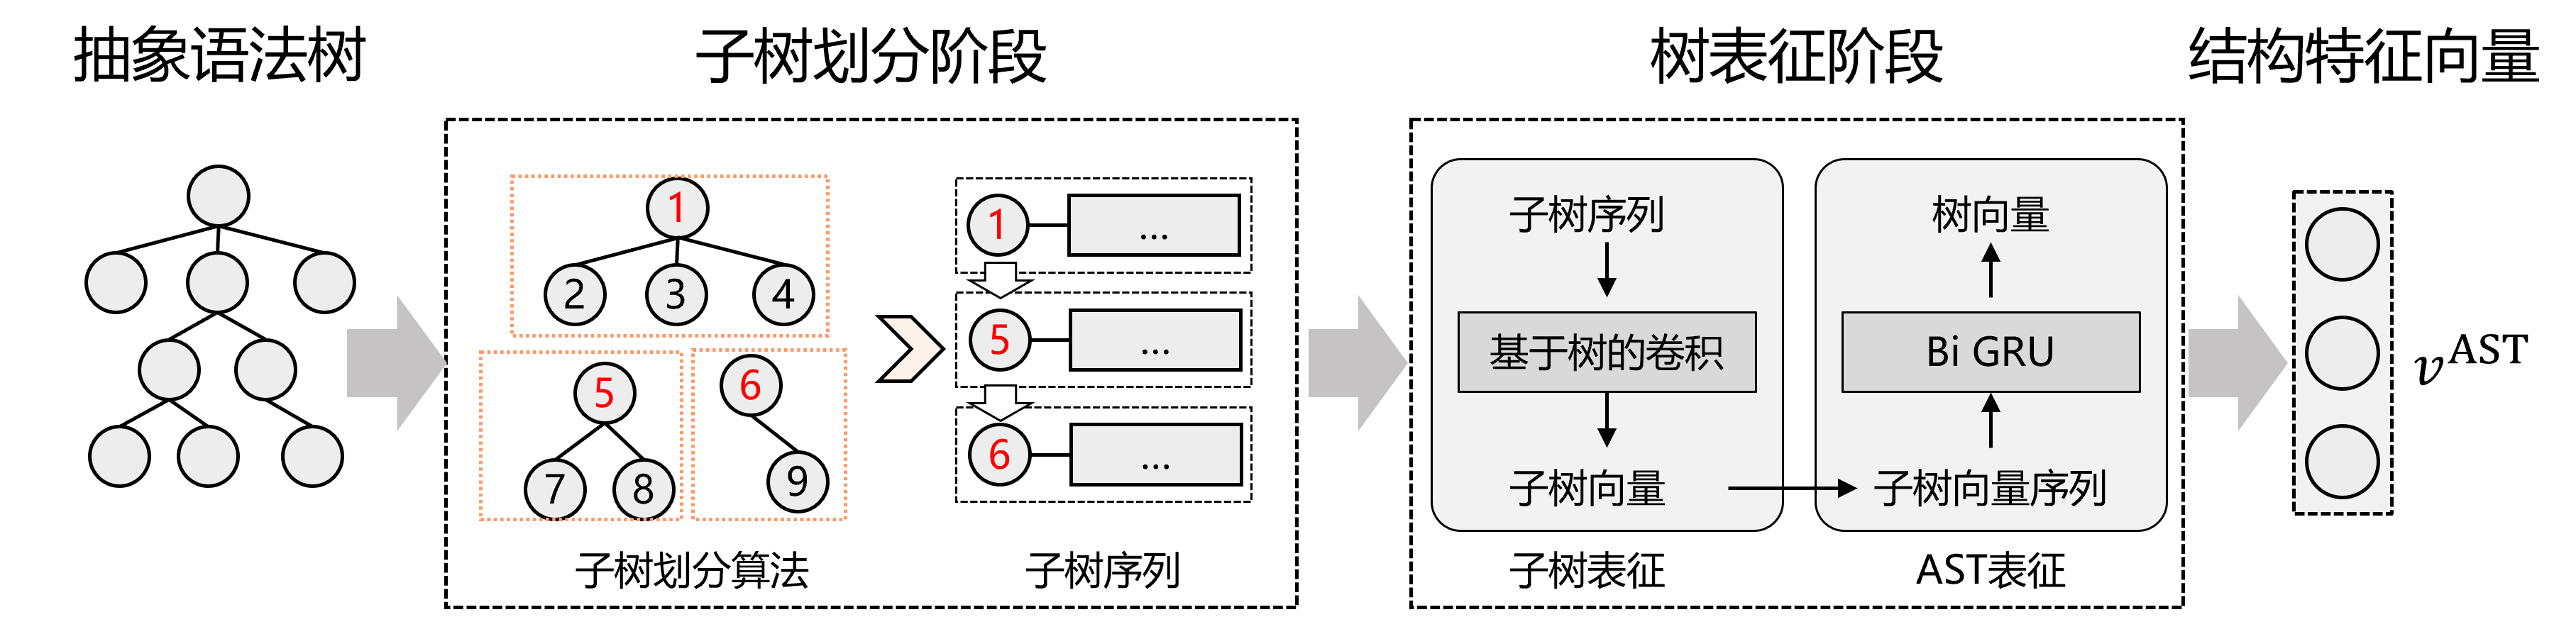
\includegraphics[width=0.95\textwidth]{figures/astframework.png}
  \caption{基于子树划分的抽象语法树表征学习框架}\label{fig:astframework}
\end{figure}

首先,子树划分阶段以代码片段对应的抽象语法树作为训练数据,以抽象语法树的声明节点和语句节点作为切割粒度,设计一个基于先序遍历的子树划分算法,将抽象语法树切分成若干子树,得到对应的子树序列。

其次,树表征阶段以子树序列作为输入,输出代码片段对应的结构特征向量。该阶段分为两个部分,首先针对每一个子树,构建一个基于树的卷积神经网络将子树编码成向量,实现对细粒度语义的捕捉;其次,构建一个基于双向门控循环单元(BiGRU)的神经网络模型,通过最大池化层对子树特征进行压缩,输出一个固定长度的密集向量用来表示代码的结构特征。需要注意的是,在树表征阶段,本文使用两种神经网络模型,前者在语句粒度上对代码信息进行特征提取,后者引入在GRU模型的基础上引入双向结构,从而更好地捕捉序列数据的双向依赖关系。

在上述框架中,本文的创新点主要体现在子树划分阶段的子树划分算法、树表征阶段的树卷积、BiGRU模型设计两方面,下面将围绕这两个创新点来阐述本文的方法。

\subsection{子树划分设计}
\label{subsec:ASTPreModel}

抽象语法树是源代码语法结构的一种抽象表现形式,以树的形式包含了源代码中的语法信息和语法结构,不同的节点类型代表了源代码中的不同元素。其中,声明节点和语句节点是两种关键的节点类型。

声明节点用来定义代码中变量、函数、类等元素的声明,不仅包含了声明的标识符名称,还包含了该标识符的类型信息、作用域以及可能的初始值等。例如,在编译时,编译器可以通过检查声明节点来确保变量在使用前已经被正确声明,并且其类型与使用场景相匹配。

语句节点则用来定义代码的执行语句,如赋值语句、条件语句、循环语句、函数调用等。在AST中,语句节点通常包含了语句的类型、操作数以及可能的控制流信息。例如,在编译条件语句时,编译器可以通过分析语句节点来确定条件表达式的求值结果,并据此决定程序的执行路径。

抽象语法树存在因为树规模过大、高度过深导致的梯度消失问题,本文设计了一个基于先序遍历的子树划分算法,通过在语句粒度上对AST进行划分,在减少树高度的同时,实现对细粒度语义的捕捉。下面首先对本文提出的子树划分算法涉及到的基本元素进行定义,接着详细介绍整个算法流程。

\textbf{定义4.1.}抽象语法树语句节点集合:对于一个代码片段的AST,假设该AST的节点集合为$T = \left\{T_1,T_2,\ldots,T_n\right\}$,影响子树划分标准的语句节点包括:块语句、FOR循环语句、While循环语句、条件语句、返回语句,因此本文定义这些不同类型语句节点构成集合$S = \left\{BlockStatement,IfStatement,WhileStatement,ForStatement,\notag \right.\\\left.ReturnStatement\right\}$。

具体来说,子树划分算法需要寻找一个子树节点集合,表示为$SubT = \left\{SubT_i |\notag \right.\\\left. SubT \in T, SubT \in S,i=1,2,\ldots,k\left(k<n\right)\right\}$,其中集合$SubT$通过先序遍历AST节点获得,$n$表示AST中节点的总数量。

子树划分$split\_AST$算法的伪代码如\ref{alg2}所示,该算法有两个输入:根节点$Root\_Node$、语句节点集合$S$,输出为子树序列$SubTrees$。该算法的目的是按照先序遍历抽象语法树,根据给定的语句节点集合$S$,从根节点$Root\_Node$开始,判断每个子节点$child\_node$,是否需要将其作为新的子树进行切分(算法第4行),如果子节点属于语句节点集合,则直接加入子树节点集合中(算法第5行),否则需要继续遍历,找到包含子节点的子树,进行递归切分(算法第11行),最终得到子树节点列表,即子树序列$SubTrees$。

\begin{algorithm}[ht]  
	\renewcommand{\algorithmicrequire}{\textbf{Input:}}
	\renewcommand{\algorithmicensure}{\textbf{Output:}}
	\caption{Subtree partitioning algorithm $\left(split\_AST\right)$}  
	\label{alg2}
	\begin{algorithmic}[1]
    \Require Root node of abstract syntax tree:$Root\_Node$
    \Require Node set:$S$
		\Ensure SubTree set:$SubTrees$
    \State $SubTrees = \left\{\right\} $    
    \State SubTrees.append$\left(Root\_Node\right)$
		\For{child\_node $in$ Root\_Node.children}
      \If {child\_node $\in$ S} \Comment{判断是否是语句节点}
        \State SubTrees.append$\left(child\_node\right)$
      \Else
        \For{subtree $in$ SubTrees} \Comment{继续遍历子树}
          \If {child\_node $\in$ SubTrees.descendant}
            \State SubTrees.append$\left(child\_node\right)$
          \Else
            \State $ split\_AST\left(subtree\right)$ \Comment{递归切分}
          \EndIf
        \EndFor
      \EndIf
    \EndFor \\
    \Return $SubTrees$
	\end{algorithmic}
\end{algorithm}

具体地,如图\ref{fig:astshili}所示,(a)为示例代码片段,(b)为利用代码分析工具Joern生成得到抽象语法树T,(c)为利用子树划分算法将其切分为一系列子树SubT。其中,以Method为根节点,其名称为main,body节点则代表了内部代码块,该块中包含三棵变量声明子树(Local)、一棵FOR循环条件子树(ForStatement)、一棵函数声明子树(Function)以及返回语句子树(ReturnStatement),而FOR循环条件子树内部包含一课If条件句法子树(IfStatement)。

\begin{figure}[H]
  \centering
  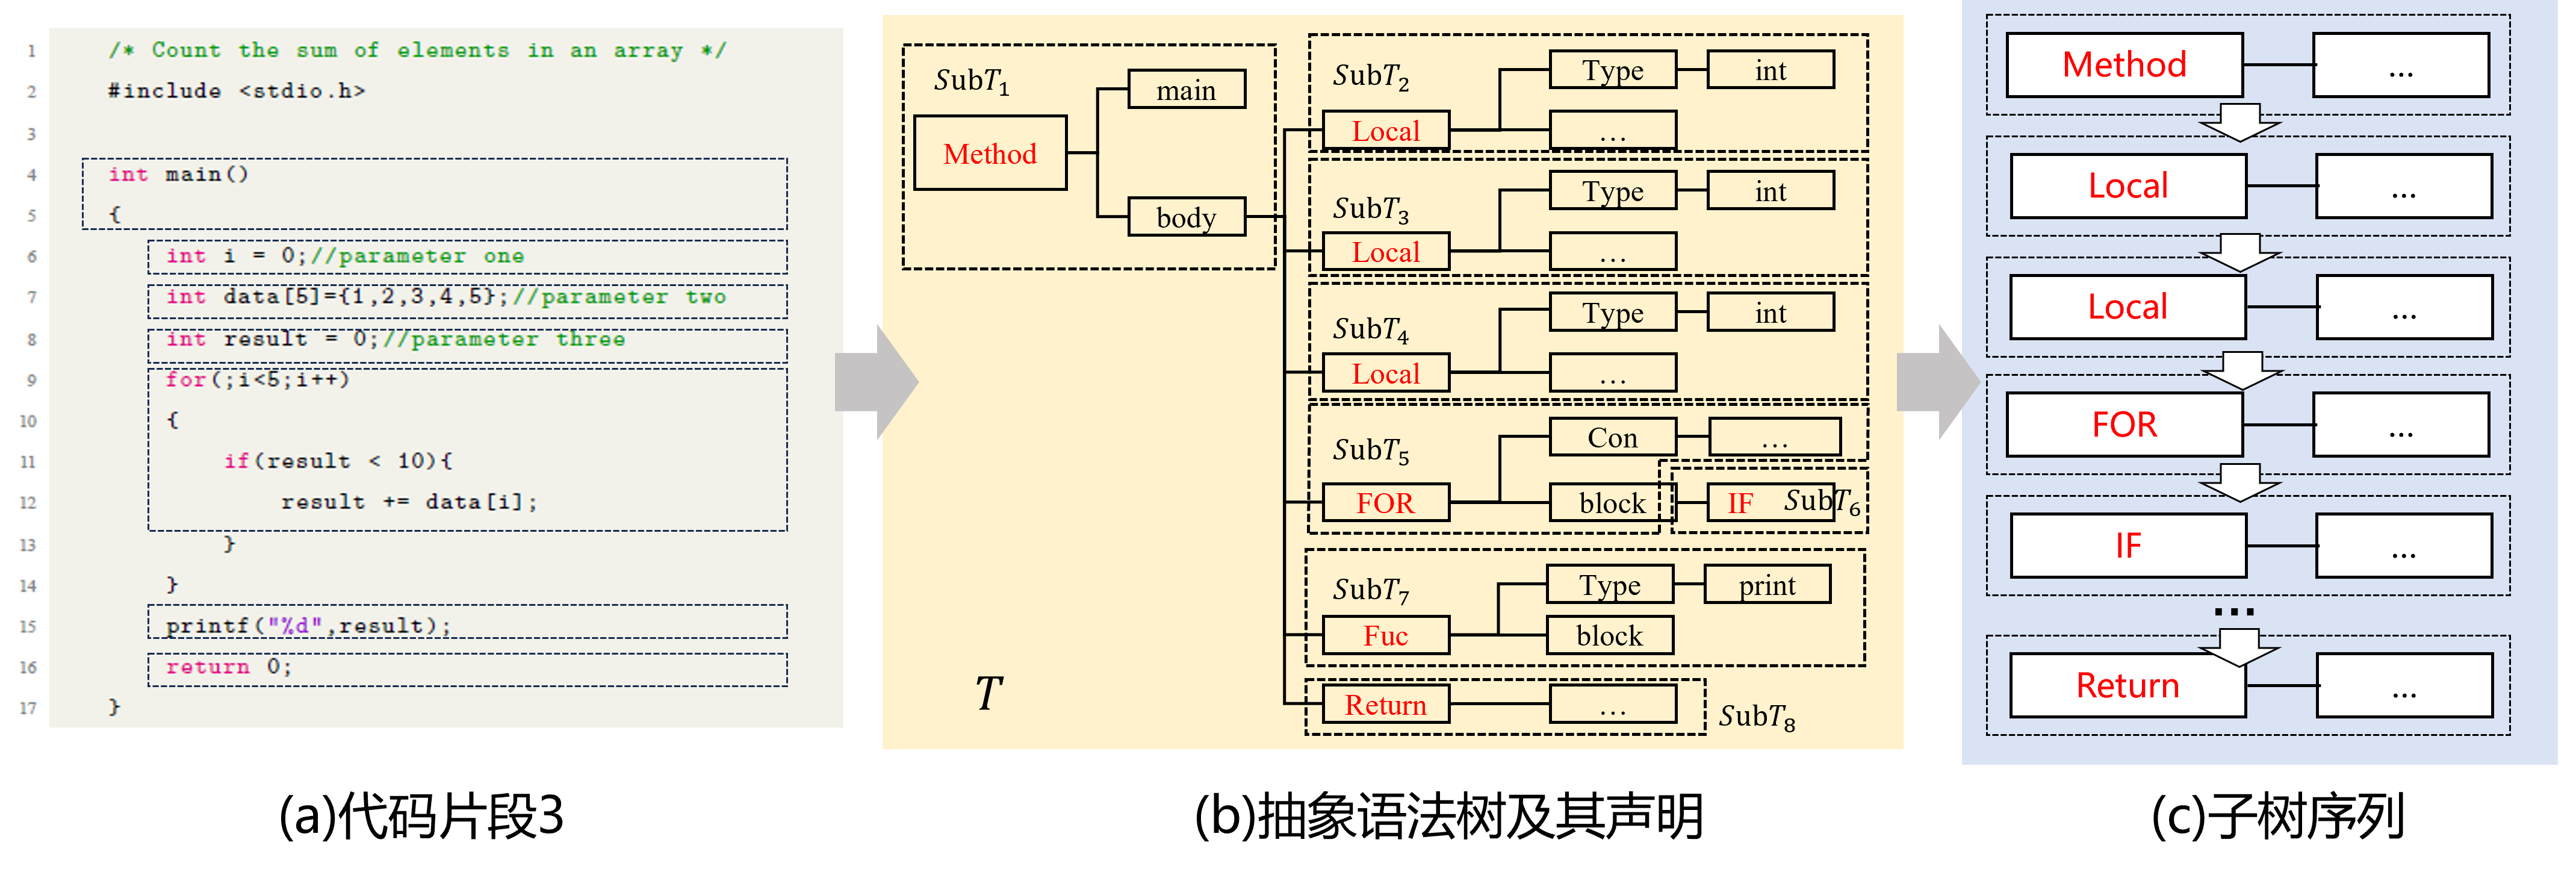
\includegraphics[width=0.95\textwidth]{figures/astshili.png}
  \caption{子树划分算法示例}\label{fig:astshili}
\end{figure}

% \lstset{language=C}
% \begin{lstlisting}
%     /* Count the sum of elements in an array */
%     #include <stdio.h>
    
%     int main()
%     {
%         int i = 0;//parameter one
%         int data[5]={1,2,3,4,5};//parameter two
%         int result = 0;//parameter three
%         for(;i<5;i++)
%         {
%             if(result < 10){
%                 result += data[i];
%             }
%         }
%         printf("%d",result); 
%         return 0;
%     }
% \end{lstlisting}

\subsection{抽象语法树表征学习设计}
\label{subsec:ASTModel}
(1)结构设计

为了提高抽象语法树维度代码表征能力,本文选取树卷积网络对上述得到子树序列进行建模,使用双向门控循环单元(BiGRU)对整个树进行建模。具体的模型设计如图\ref{fig:astmodel}所示。该模型主要包括输入层、子树卷积层、双向门控循环层(BiGRU)、最大池化层、输出层。
\begin{figure}[H]
  \centering
  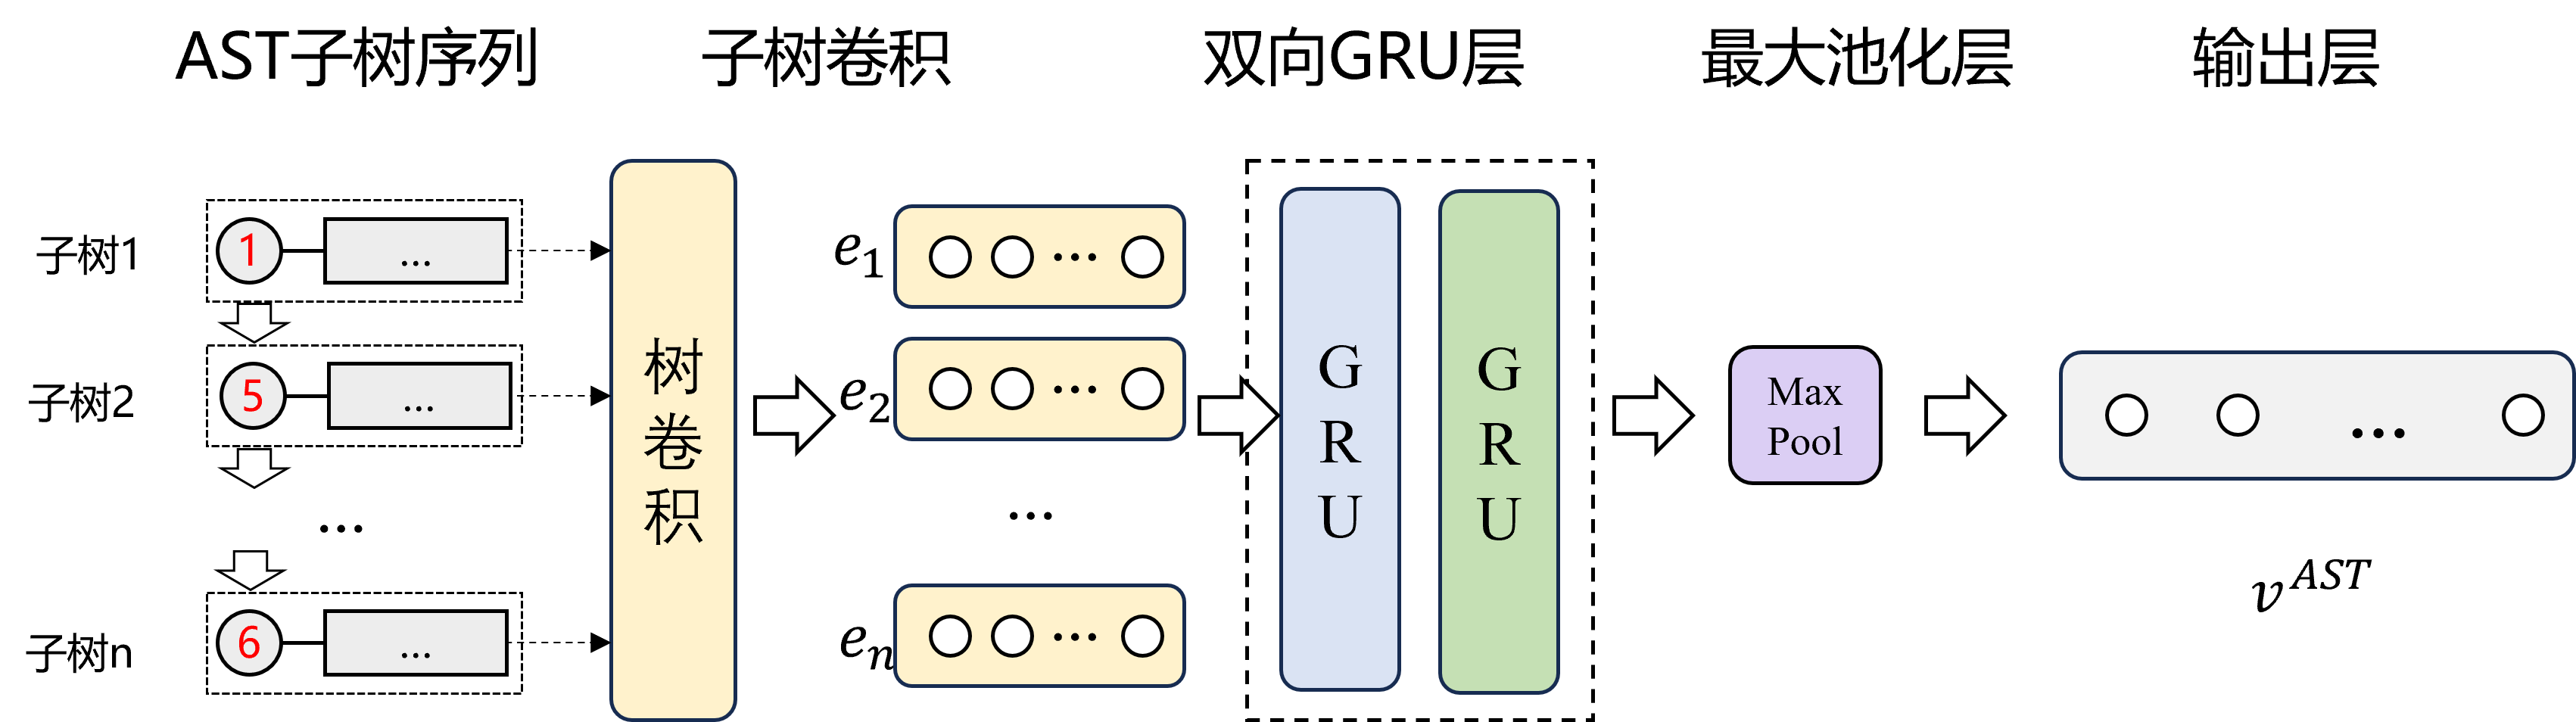
\includegraphics[width=0.85\textwidth]{figures/astmodel.png}
  \caption{抽象语法树维度代码表征模型结构}\label{fig:astmodel}
\end{figure}

\ding{172}输入层:输入层用于向模型输入训练数据,在本方法中模型的输入为经过子树划分得到的子树序列。\ding{173}子树卷积层:针对子树序列中的每一个子树,通过基于树的卷积,捕获语句粒度语义信息。\ding{174}双向门控循环层:由两层GRU构成,同时捕获序列的双向语义信息。\ding{175}最大池化层:总结子树序列的输入特征,并将其缩减为一个单一的密集向量。\ding{176}输出层:每个抽象语法树对应一个输出。

(2) 模型选型

树表征阶段包含两个步骤:子树表征、整树表征。因此本文设计了两个神经网络模型:前者的输入是子树序列,针对每个子树进行基于树的卷积,在子树粒度上对代码进行信息提取;后者的输入是子树向量序列,针对所有子树的特征进行双向特征提取,并整合整棵树的信息,得到一个结构特征向量。

(2.1)子树表征模型

卷积神经网络(Convolutional Neural Network,CNN)是一种深度学习模型,其架构包括多个卷积层、池化层和全连接层。其中,卷积层负责从输入数据中提取特征,池化层用于降低数据维度,全连接层则用于将前面各层的特征映射到输出空间。其中,卷积思想是指将一个固定大小的窗口(通常被称为卷积核)在输入数据上按照一定的步长进行滑动,并对每个窗口中的局部片段进行特征提取,最后得到一系列特征,每个特征对应一个卷积核提取的特征。它能够将输入数据从底层到高层逐步抽象化,形成层次化的特征表示。

常见的卷积核通常都是正方形的,但树形结构通常是不规则,因此有研究\cite{8813290}提出了基于树的卷积神经网络。该网络的核心思想是将卷积操作扩展到树形结构上。通过定义在树上的卷积核,可以捕获树的节点与其邻居之间的局部特征。这种局部感知的方式与传统的卷积神经网络类似,但不同的是,其卷积核是三角形的,能够在不规则的树形结构上进行。基于树的卷积如下图\ref{fig:TreeBaseConvolution}所示。

\begin{figure}[H]
  \centering
  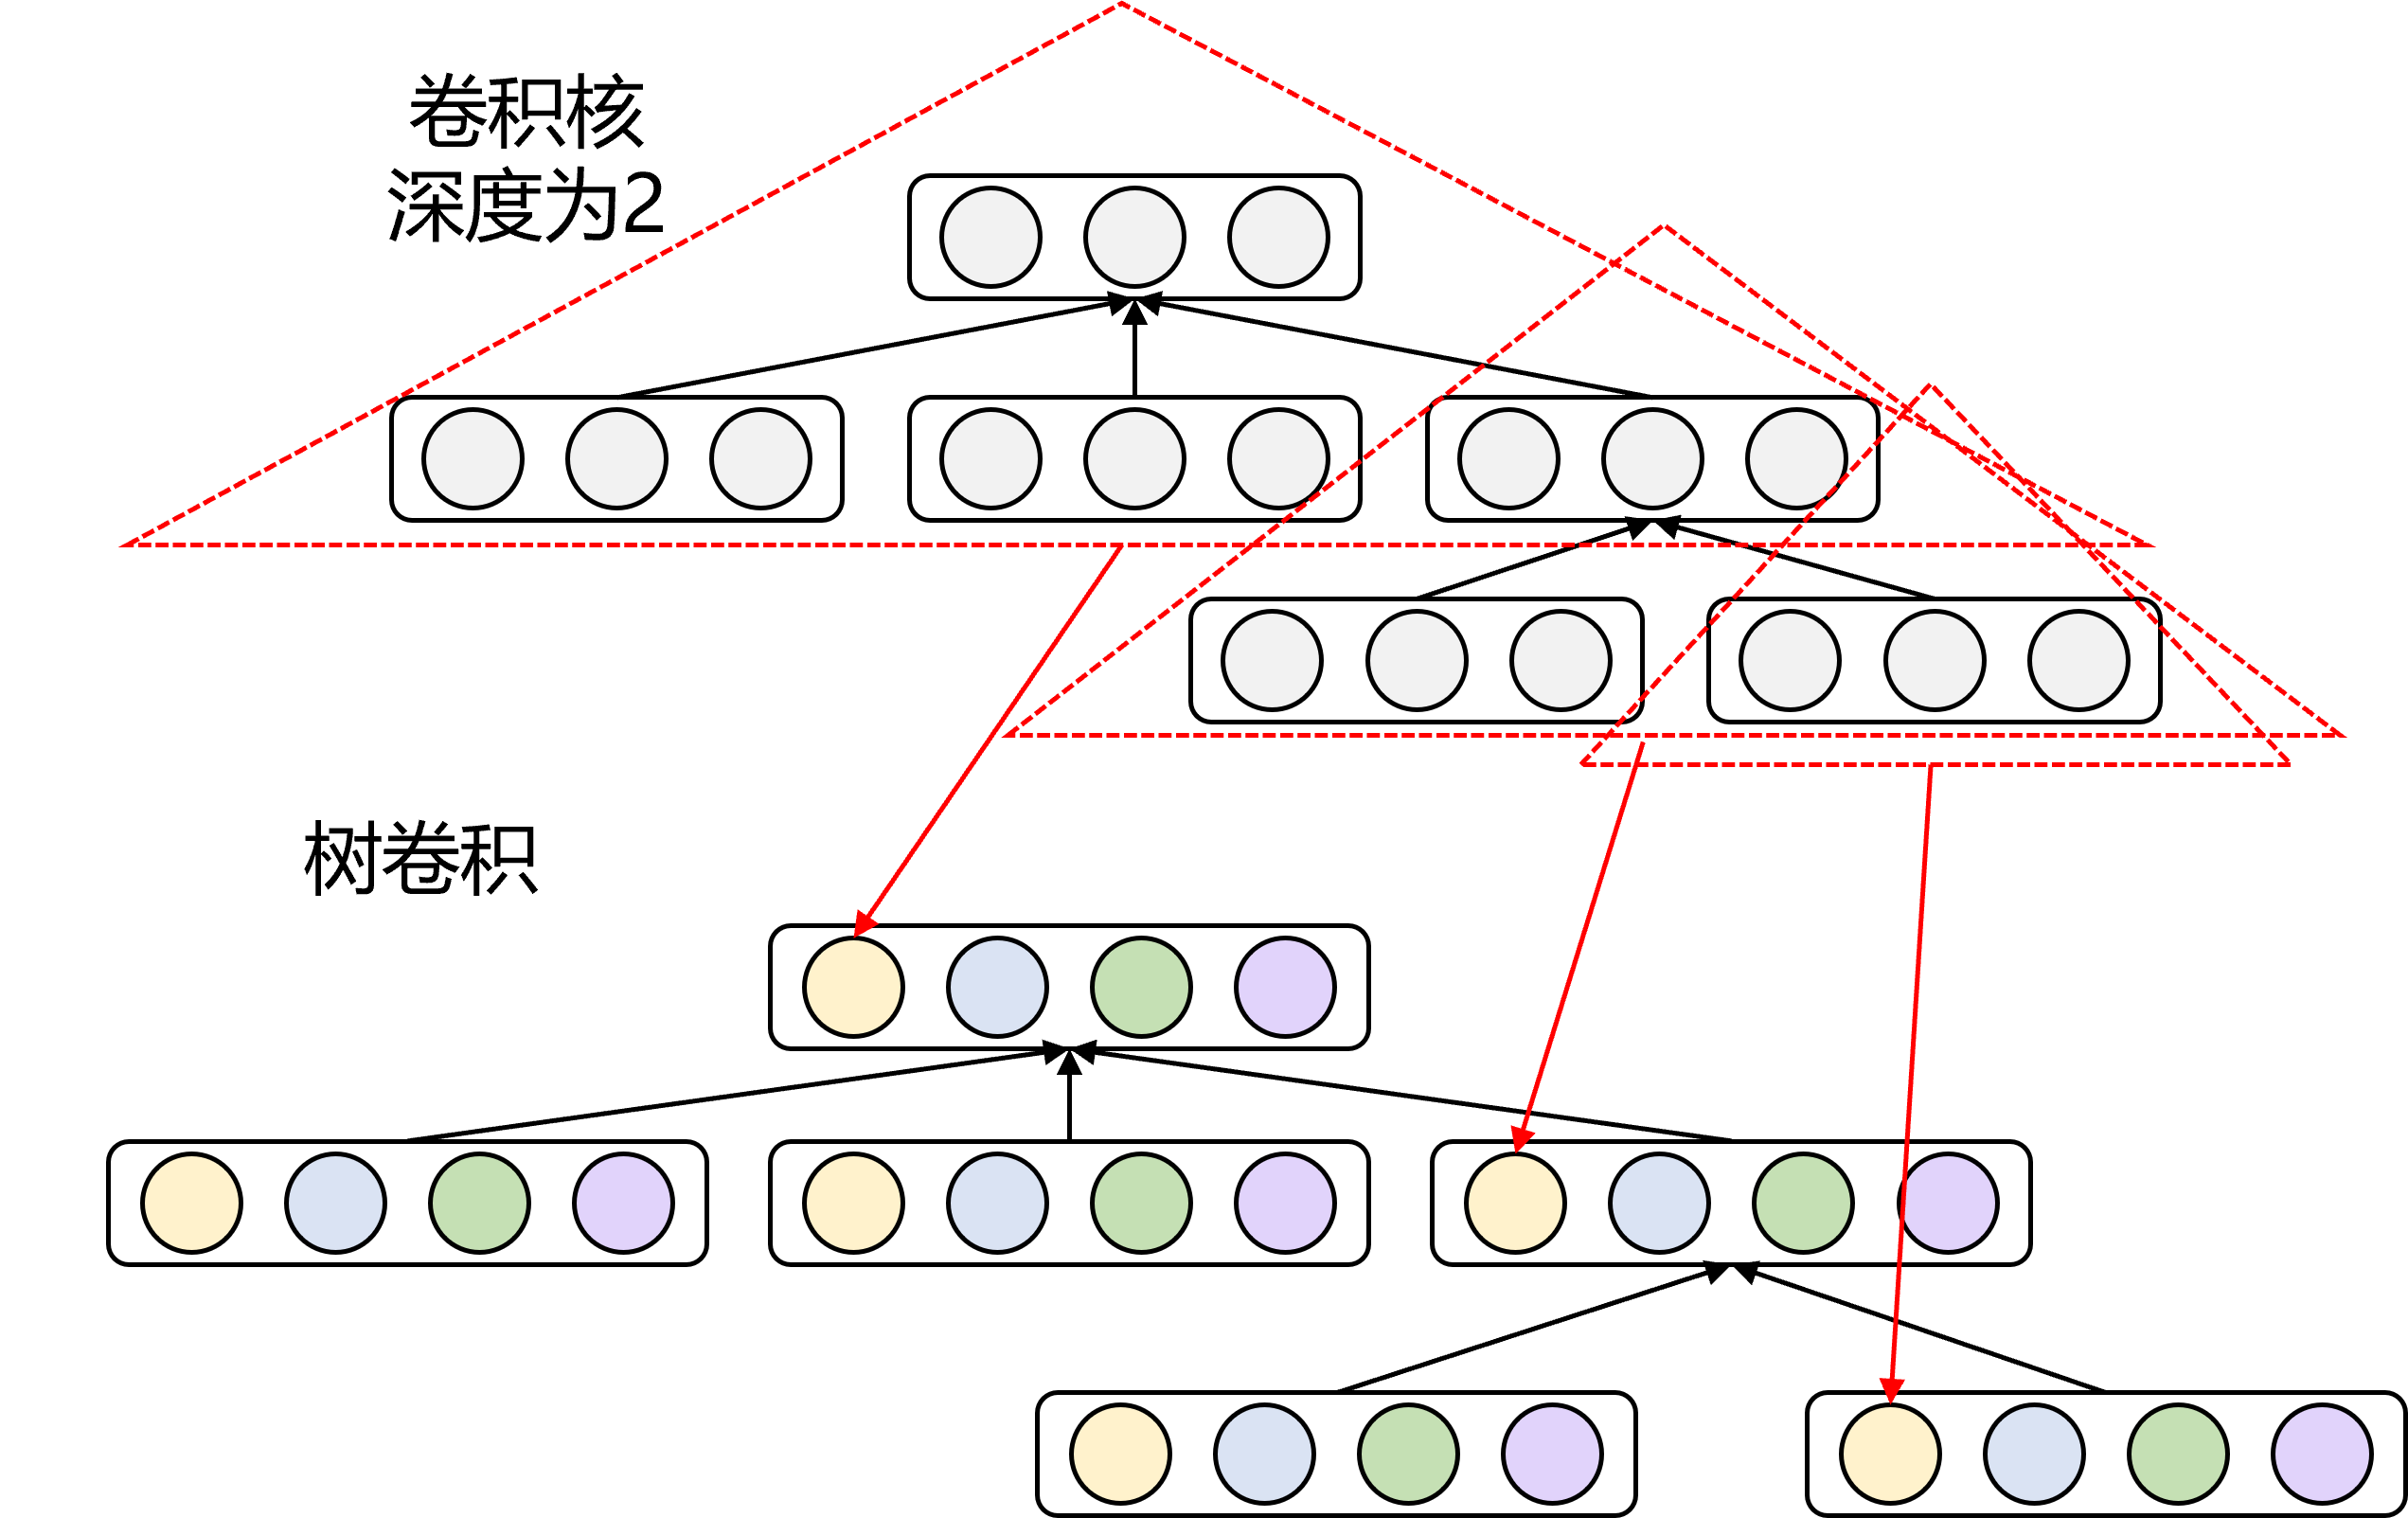
\includegraphics[width=0.65\textwidth]{figures/TreeBaseConvolution.png}
  \caption{基于树的卷积神经网络模型结构}\label{fig:TreeBaseConvolution}
\end{figure}

在基于树的卷积神经网络中,每个节点都与其邻居节点相连,形成一个局部邻域。卷积核在这个局部邻域上进行滑动,计算节点与其邻居的加权和,从而提取出特征。用数学公式表示,卷积核的滑动尺寸是$d$,它表示每个滑动窗口能够包括的树的层数。在这个窗口内包含$n$个节点$\left(x_1,x_2,\ldots,x_n\right)$,其中,$x_i \in \mathbb{R}^{N_{f}}$,$N_{f}$表示每个节点建模后的向量大小。使用公式\ref{e4.1}可以对滑动窗口内$n$个节点进行卷积得到基于树的卷积神经网络输出。
\begin{equation}\label{e4.1}
  \begin{split}
    y = \tanh \left(\sum_{i=1}^{n} W_{\text{conv}, i} \cdot x_{i}+b_{\text{conv}}\right)
  \end{split}
\end{equation}

其中,$y, b_{\text{conv}} \in \mathbb{R}^{N_{f}}, W_{\text{conv}, i} \in \mathbb{R}^{N_{c} \times N_{f}}$,$N_{c}$为最后卷积得到的向量长度。具体地,在上图\ref{fig:TreeBaseConvolution}的例子中,红色三角形表示卷积核,固定深度$d$为2,最后输出的卷积向量长度$N_{c}$为4。树结构在卷积前后保持相同的形状,而每个节点向量的维数由原来的3维变为4维。

基于树的卷积网络模型存在一个限制:其子节点的数量被限制为两个。但实际上,AST理论上可以存在无限数量的子节点,每次滑动窗口中的节点数$n$难以固定,从而导致无法确定权重矩阵的数量,即公式\ref{e4.9}中的$W_{conv,i}$。现有研究的解决方法是预先定义一组规则将抽象语法树转化为二叉树,然后再进行树卷积。这种处理方式,会改变源代码原有的语义,从而难以捕捉远程依赖关系,甚至丢失一些上下文信息,因此本文采用研究\cite{8813290}中提出的连续二叉树概念,将AST的每一个子树都看作二叉树,而不管它的形状和尺寸。图\ref{fig:Continuous}展示了连续二叉树的定义。

\begin{figure}[H]
  \centering
  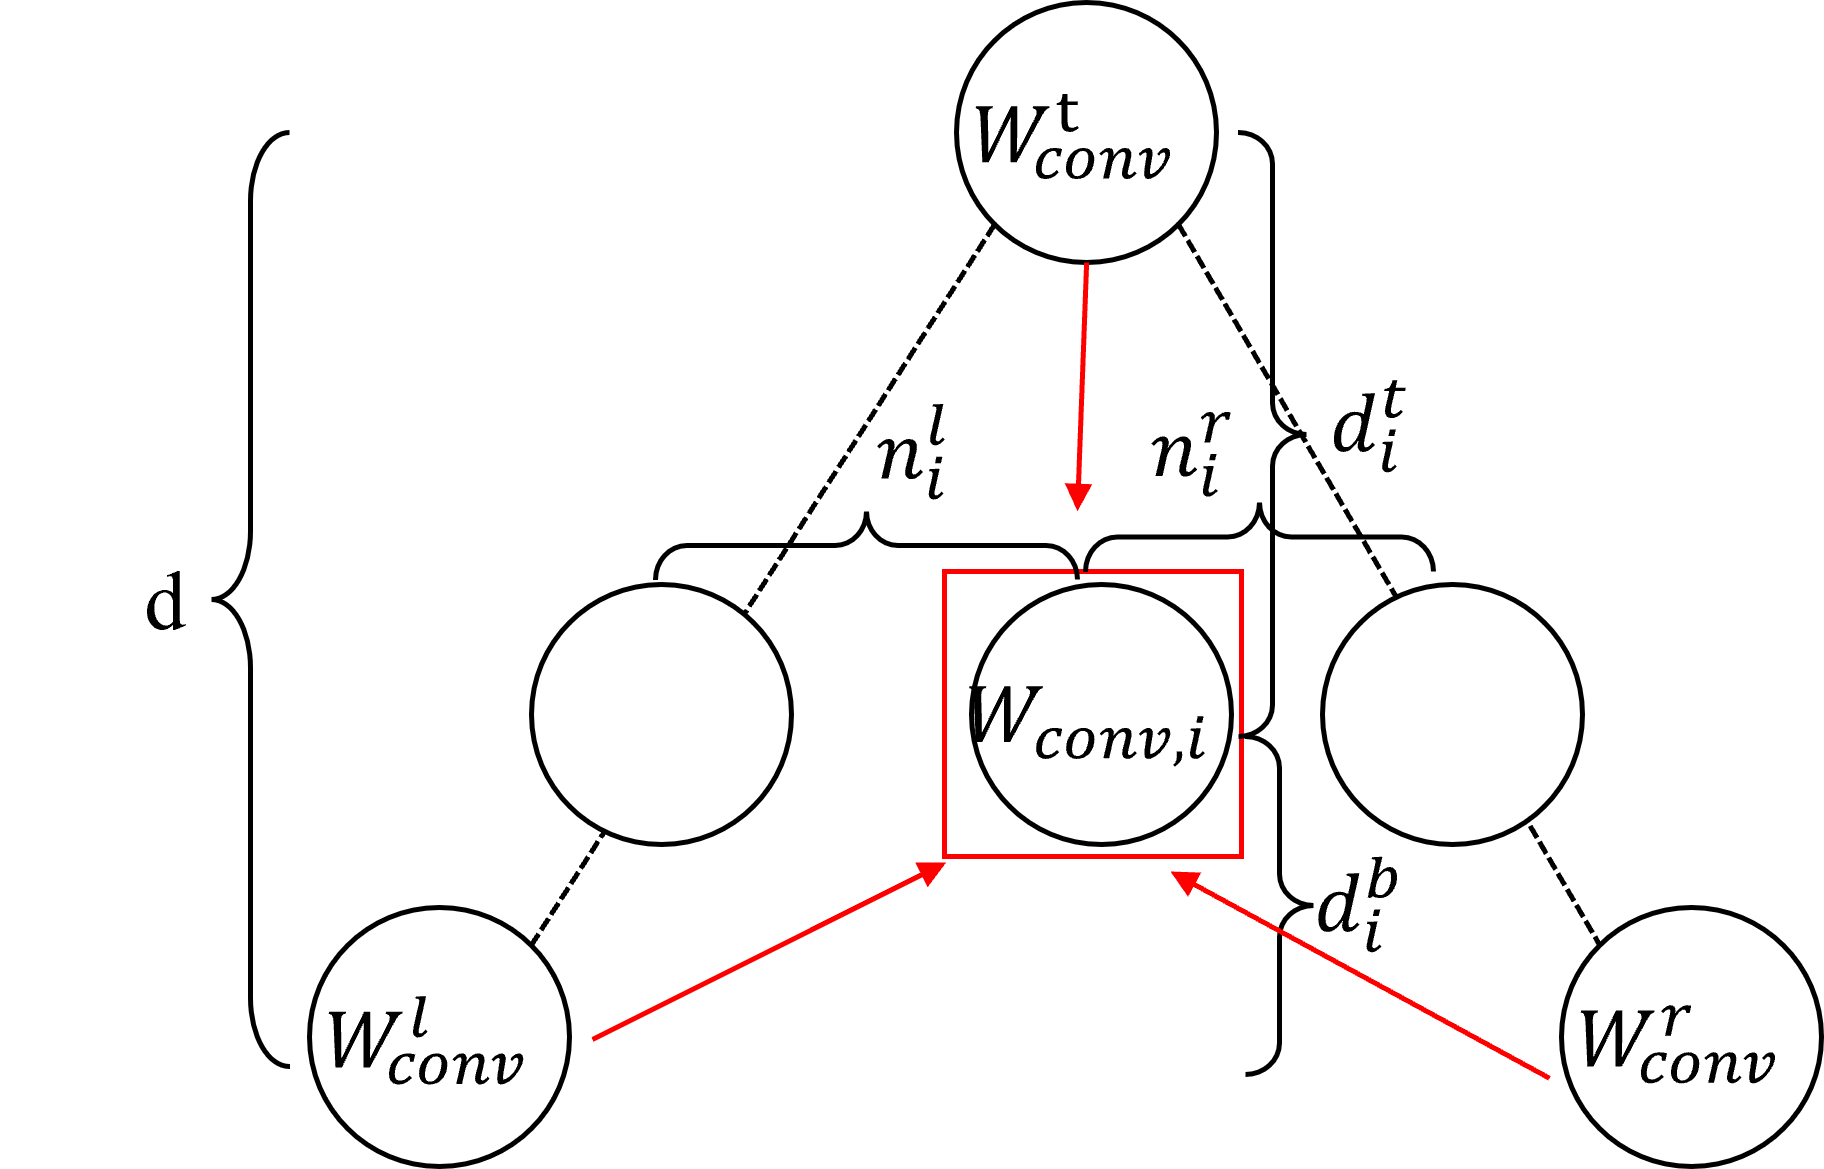
\includegraphics[width=0.6\textwidth]{figures/Continuous Binary Tree.png}
  \caption{连续二叉树}\label{fig:Continuous}
\end{figure}

具体地,针对滑动窗口中的节点,需要设置三个变量:$W_{\text{conv}}^{t},W_{\text{conv}}^{l},W_{\text{conv}}^{r}$分别代表当前节点距离树形上、左、右三个方向,其卷积矩阵$W_{conv,i}$是这三个变量的线性组合,其系数根据节点在当前滑动窗口中的相对位置计算,具体公式为\ref{e4.2}:
\begin{equation}\label{e4.2}
  \begin{split}
    W_{\text{conv}, i}=\frac{d_{i}^{b}}{d_{i}^{b}+d_{i}^{t}} W_{\text{conv}}^{t}+\frac{d_{i}^{t}}{d_{i}^{b}+d_{i}^{t}} W_{\text{conv}, i}^{b}
  \end{split}
\end{equation}

其中,$d_{i}^{t}$表示当前节点距离树形顶点的距离,$d_{i}^{b}$表示当前节点距离树形左右顶点构成的边的距离,两者相加为$d$,即$d_{i}^{t} + d_{i}^{b} = d$。上式中$W_{\text{conv}, i}^{b}$有如下定义:

\begin{equation}\label{e4.3}
  \begin{split}
    \begin{array}{l}
      W_{\text{conv}, i}^{b}= 
      \left\{\begin{array}{ll}
      \frac{n_{i}^{r}}{n_{i}^{r}+n_{i}^{l}} W_{\text {conv}}^{l}+\frac{n_{i}^{l}}{n_{i}^{r}+n_{i}^{l}} W_{\text{conv}}^{r} & n_{i}^{l} \geq 1 \text { or } n_{i}^{r} \geq 1, \\
      \frac{1}{2} W_{\text{con}}^{l}+\frac{1}{2} W_{\text{conv}}^{r} & n_{i}^{l}=n_{i}^{r}=0 .
      \end{array}\right.
      \end{array}
  \end{split}
\end{equation}

其中,$n$表示树的同一层左右两个方向的兄弟节点个数。通过上述公式,可以计算在一个三角形的卷积窗口中,当节点越接近顶点,其$W_{\text{conv}}^{t}$的权重值越大,当节点越接近树形结构左下节点,其$W_{\text{conv}}^{l}$的权重值越大,当节点越接近树形节点结构右下节点,其$W_{\text{conv}}^{r}$的权重值越大。在具体实验中,本文设置滑动窗口的$d$值为2。

(2.2)整树表征模型

\ref{subsec:TokenModel}小节中提到长短期记忆网络LSTM模型针对长依赖问题效果明显,解决了传统RNN模型中存在的梯度消失问题,但是LSTM模型同样存在缺陷,其LSTM单元内包含三个门,机制相对复杂,计算成本会有所提高,因此,有研究提出了门控循环单元GRU,将遗忘门和输入门进行组装,形成一个新的更新门,这种改进使得GRU在模型参数和计算效率上通常优于LSTM。GRU单元的时序结构如下如\ref{fig:GRU}所示,每个GRU单元都包含两个门:重置门(Reset Gate)和更新门(Update Gate),通过重置门和更新门来直接控制信息的流动和隐藏状态的信息更新。

\begin{figure}[H]
  \centering
  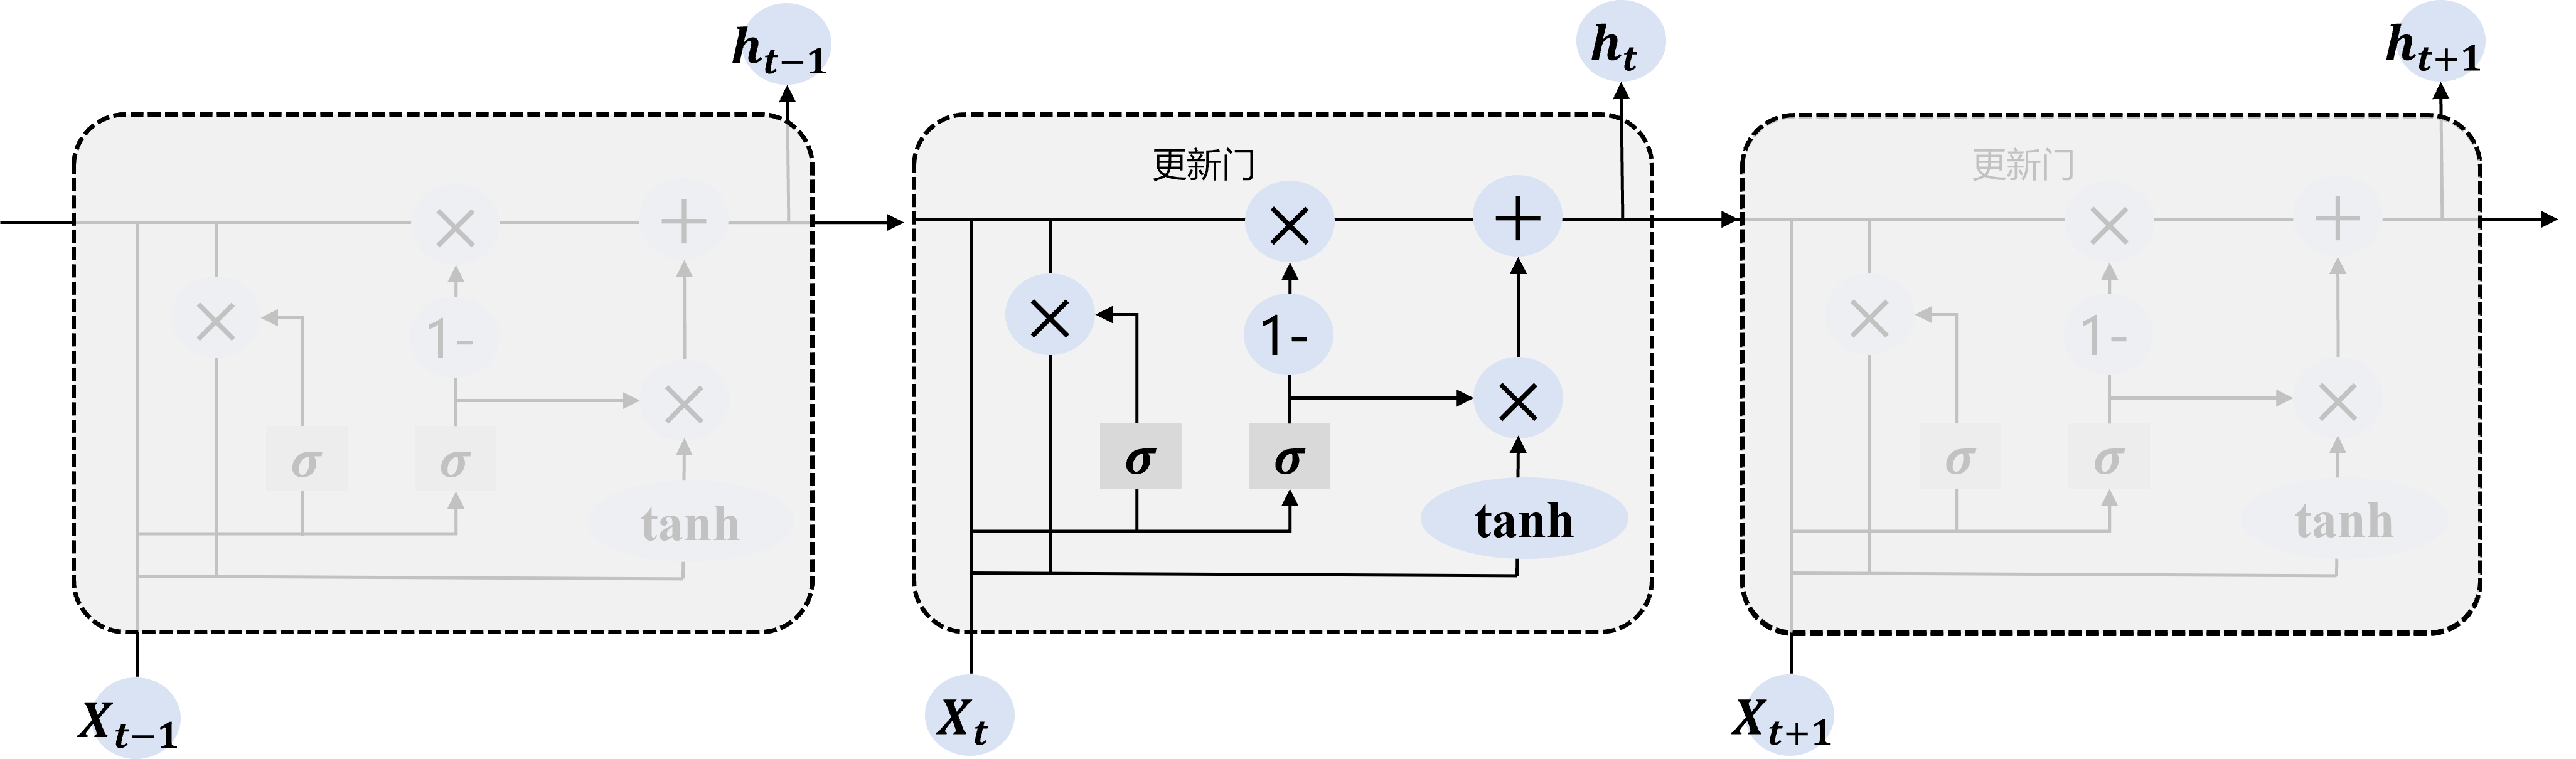
\includegraphics[width=0.85\textwidth]{figures/GRU.png}
  \caption{GRU模型时序结构图}\label{fig:GRU}
\end{figure}

具体来说,首先会根据当前时间步的输入$x_{t}$和上一时间步的隐藏状态$h_{t-1}$计算出重置门和更新门的值,具体的计算公式见\ref{e4.4}。
\begin{equation}\label{e4.4}
  \begin{split}
    z_{t} = \sigma \left(W_{u} \cdot \left[h_{t-1},x_{t}\right] + b_z \right)
    \\
    r_{t} = \sigma \left(W_{r} \cdot \left[h_{t-1},x_{t}\right]  + b_r \right)
  \end{split}
\end{equation}

然后,输入重置门,对上一个时间步的隐藏状态进行处理,得到一个新的候选隐藏状态$\widetilde{h_t}$。其中,重置门用来控制上一个时间步的信息有多少应该被遗忘。具体地,通过公式\ref{e4.5}计算一个介于-1到1之间的值,决定上一个时间步的隐藏状态有多少信息应该被保留或遗忘,得出的值越接近0越有可能被丢弃,越接近1越有可能被记住。
\begin{equation}\label{e4.5}
  \begin{split}
    \widetilde{h_t} &= \tanh \left(W_x \cdot x_t \otimes U_h \cdot\left(r_t \cdot h_{t-1}\right) + b_h  \right)
  \end{split}
\end{equation}

接着,输入更新门,将新的候选隐藏状态$\widetilde{h_t}$和上一个时间步的隐藏状态$h_{t-1}$进行加权组合,得到当前时刻的隐藏状态$h_t$,如公式\ref{e4.6}所示。其中,更新门用来控制新输入的信息和上一个时间步的信息应该如何结合。具体地,通过公式\ref{e4.7} 决定当前时刻的隐藏状态应该有多少信息来自上一时刻的隐藏状态,以及有多少信息来自当前时刻的输入和重置门处理后的结果。通过更新门,GRU能够平衡新旧信息的影响,从而有效地捕捉序列数据中的长期依赖关系。最后,当前时刻的隐藏状态会被输出。

\begin{equation}\label{e4.6}
  \begin{split}
   h_t &= \left(1- z_t\right) \otimes h_{t-1} +  z_t \otimes \widetilde{h_t}
  \end{split}
\end{equation}

同样地,在抽象语法树中,某一个节点的状态不仅和前面层的节点状态有关,也可能和后一层的节点状态有关。为了更好地提高模型对AST子序列的表征能力,本文选择了双向BiGRU模型来进行树代码表征,模型的结构如下图\ref{fig:BiGRU}所示。BiGRU模型结构结合了双向RNN(双向循环神经网络)和GRU(门控循环单元)的优点,通过其双向结构能够更有效地学习并保持长期的信息流,从而使得当前时刻的输出与前后时刻的状态都产生联系,在处理长序列数据时表现出色,在具有较快收敛速度、较强学习能力等优点的同时,还能减少梯度消失问题。

\begin{figure}[H]
  \centering
  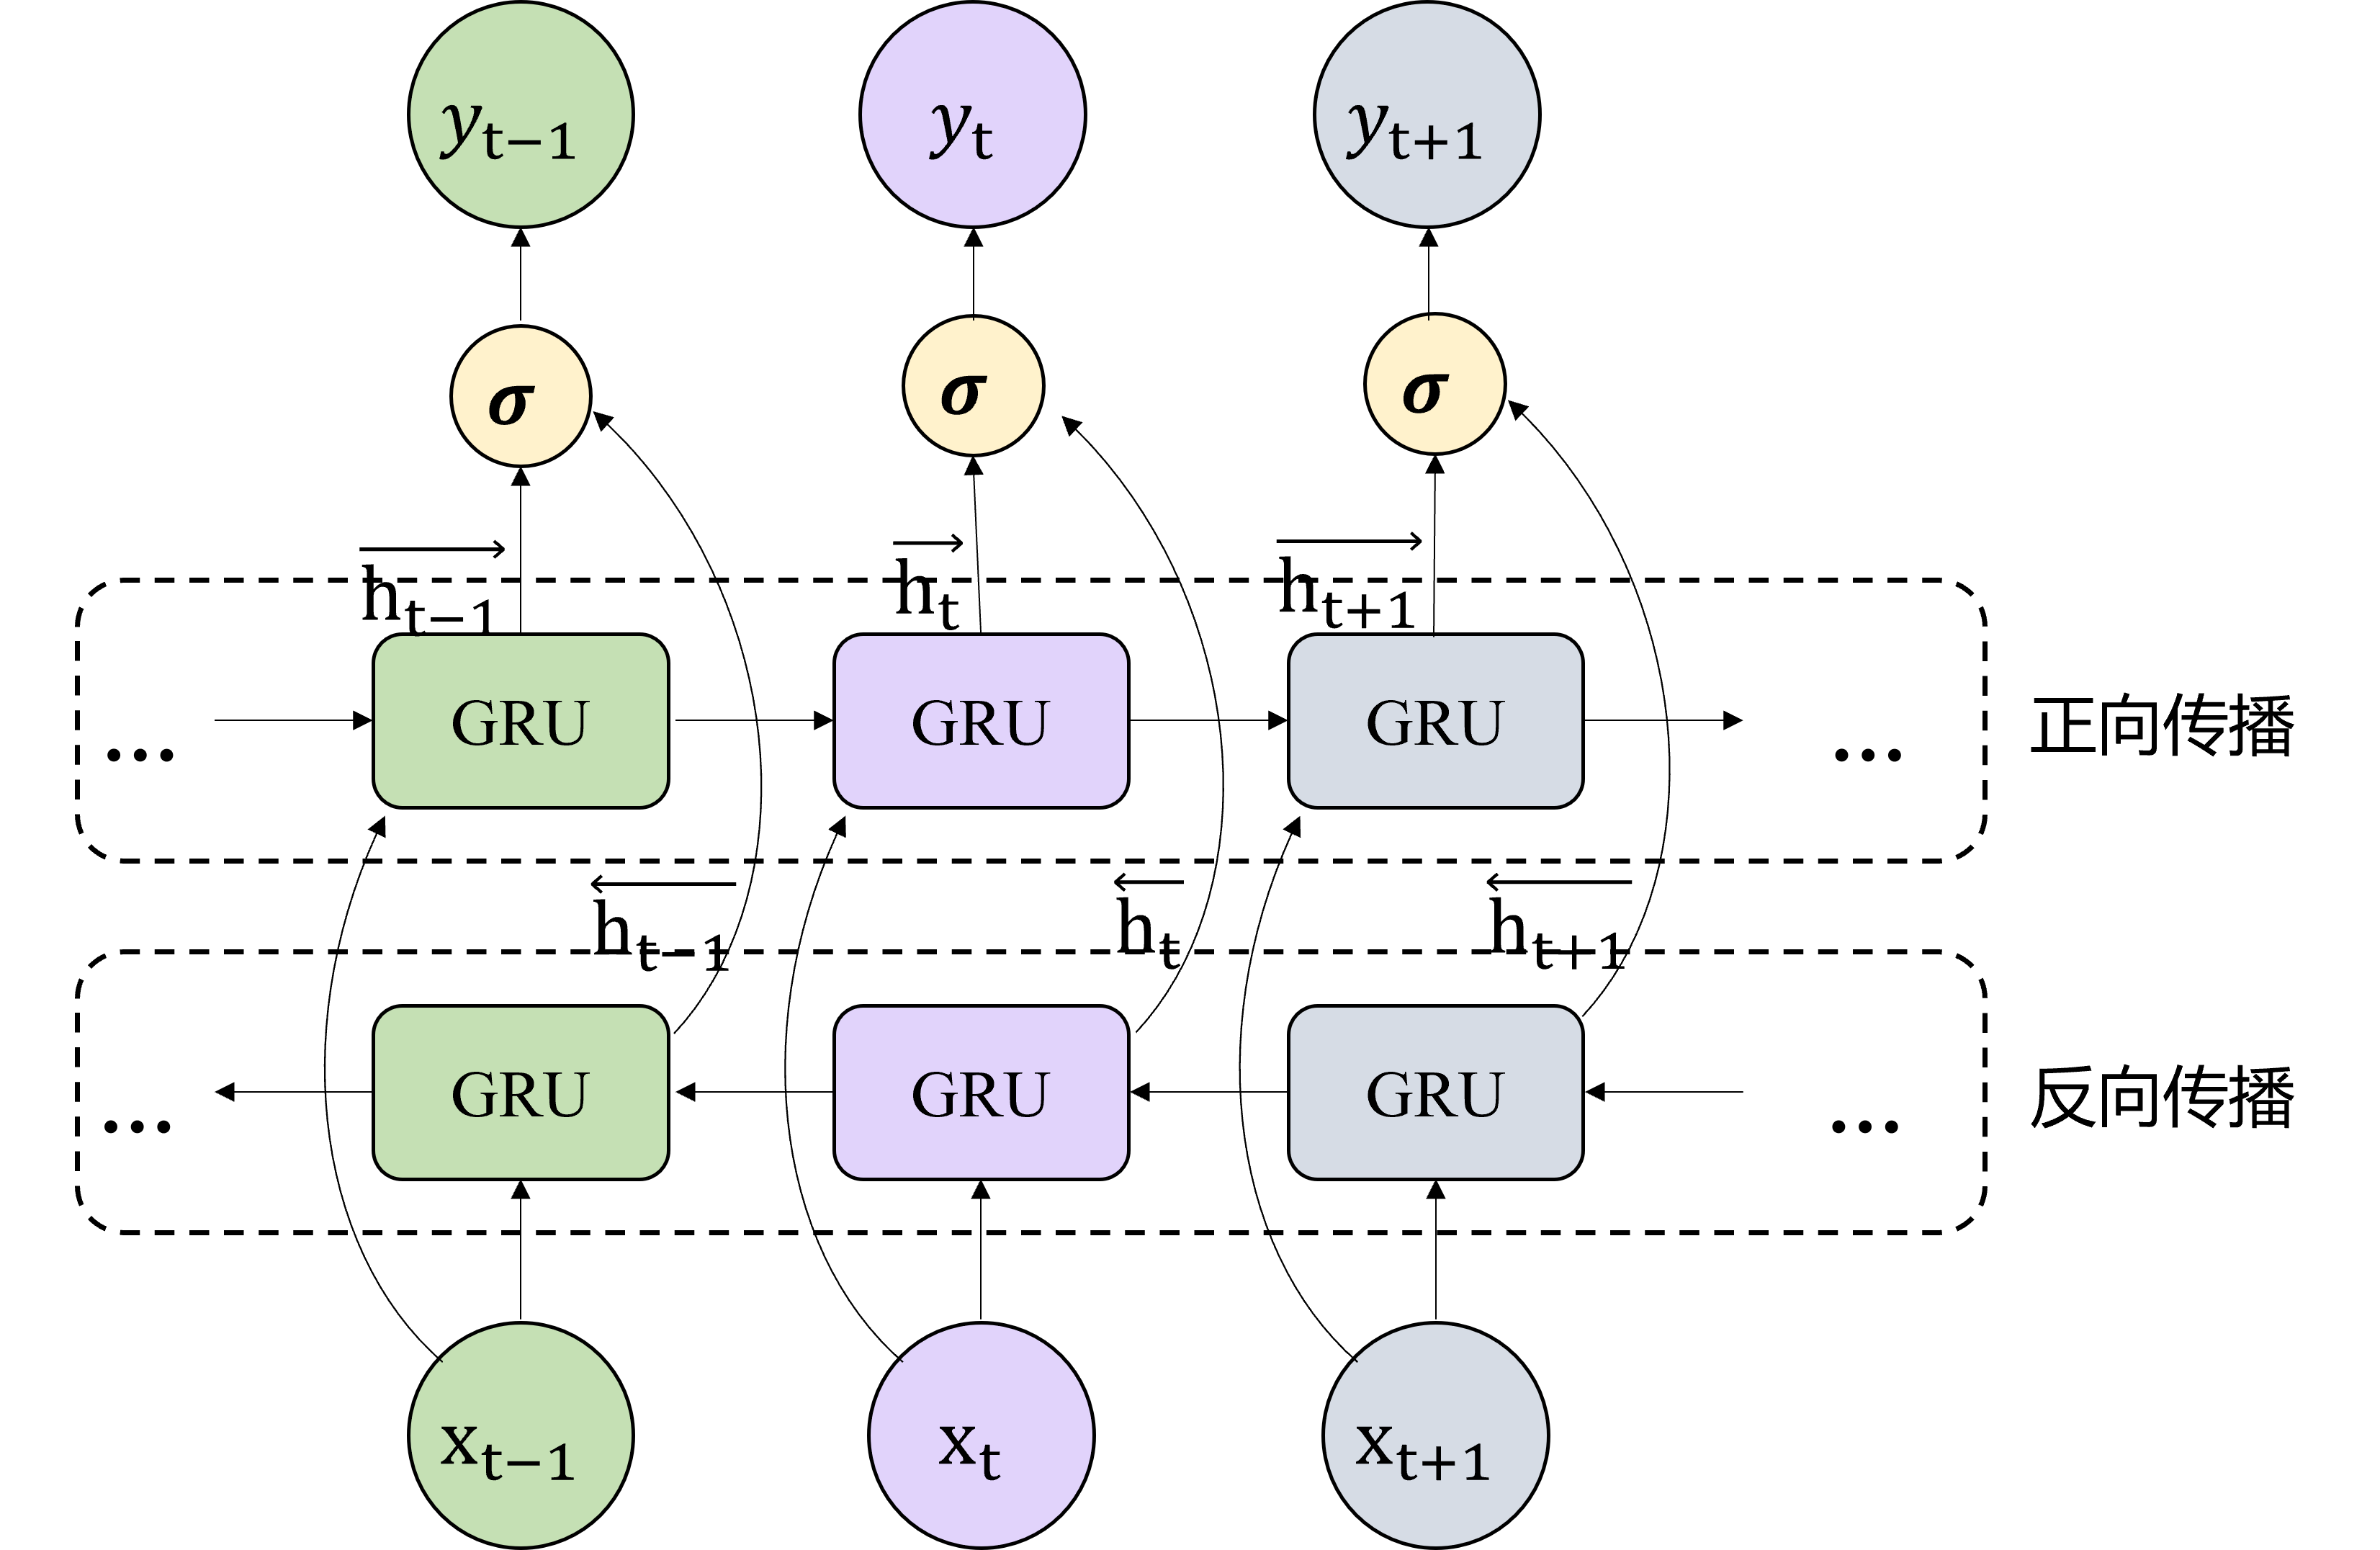
\includegraphics[width=0.5\textwidth]{figures/BiGRU.png}
  \caption{BiGRU模型结构}\label{fig:BiGRU}
\end{figure}

和\ref{subsec:TokenModel}提出的双向长短时记忆模型相比,GRU结构简单,参数简单,因此通常可以更快收敛到最优解,从而节省计算资源和时间。整个模型,除了子单元有所改变外,架构不变。这里不展开介绍,仅给出公式\ref{e4.7}。
\begin{equation}\label{e4.7}
  \begin{split}
    \overrightarrow{y_t} &= W_0 \cdot GRU\left(x_{t},\overrightarrow{h_{t-1}}\right) + b_0
    \\
    \overleftarrow{y_t} &= W_0 \cdot GRU\left(x_{t},\overleftarrow{h_{t-1}}\right) + b_0
    \\
    y_t &= \overrightarrow{y_t} \oplus\overleftarrow{y_t}
  \end{split}
\end{equation}


\section{AST表征方法具体实现}
\label{sec:ASTachieve}
在介绍具体实现之前,本节首先给出AST表征方法的输入:经过\ref{subsec:Preprocess}小节的代码预处理阶段,得到示例代码片段\ref{fig:code}对应的抽象语法树,如图\ref{fig:astcode}所示。仔细分析可以看出代码片段\ref{fig:ast1}对应的抽象语法树在FOR循环内部一共有13个子节点,子树高度为4;代码片段\ref{fig:ast2}对应的抽象语法树在WHILE循环内部也包含13个子节点,子树的高读为4,两者子节点个数相同;而代码片段\ref{fig:ast3}对应的抽象语法树在FOR循环中共有18个子节点,子树高度为6,与代码片段\ref{fig:ast1}对应的抽象语法树在根节点的下一层、下两层中1-9号节点架构相似。
\begin{figure}[htbp]
  \centering  %居中
  \subfigure[代码片段1对应的AST]{   %第一张子图
      \centering    %子图居中
      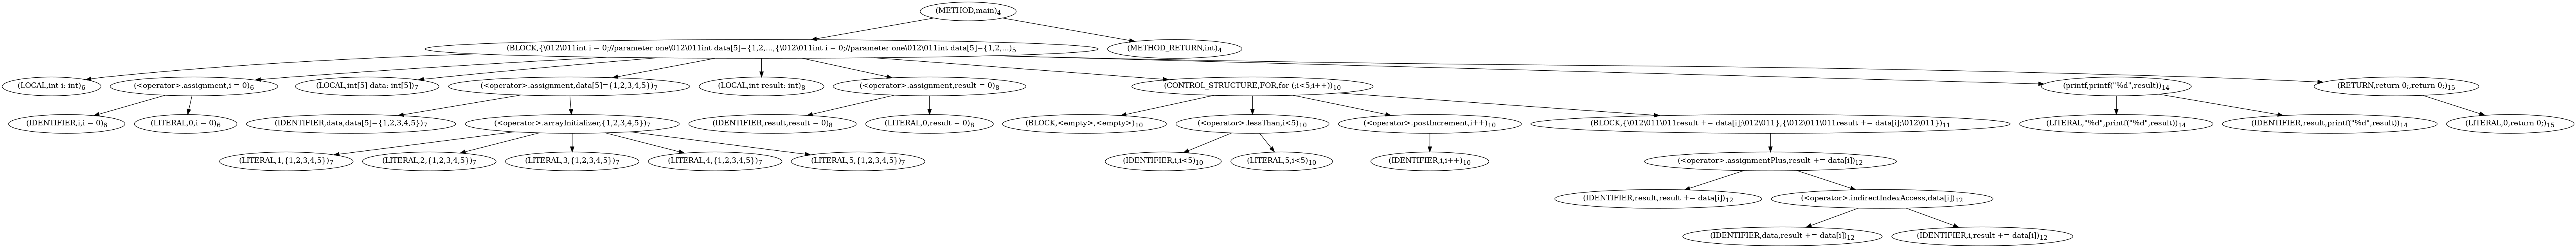
\includegraphics[width=0.3\textwidth]{figures/ast1}  
      \label{fig:ast1} %引用标签
  }
  \subfigure[代码片段2对应的AST]{ %第二张子图
      \centering    %子图居中
      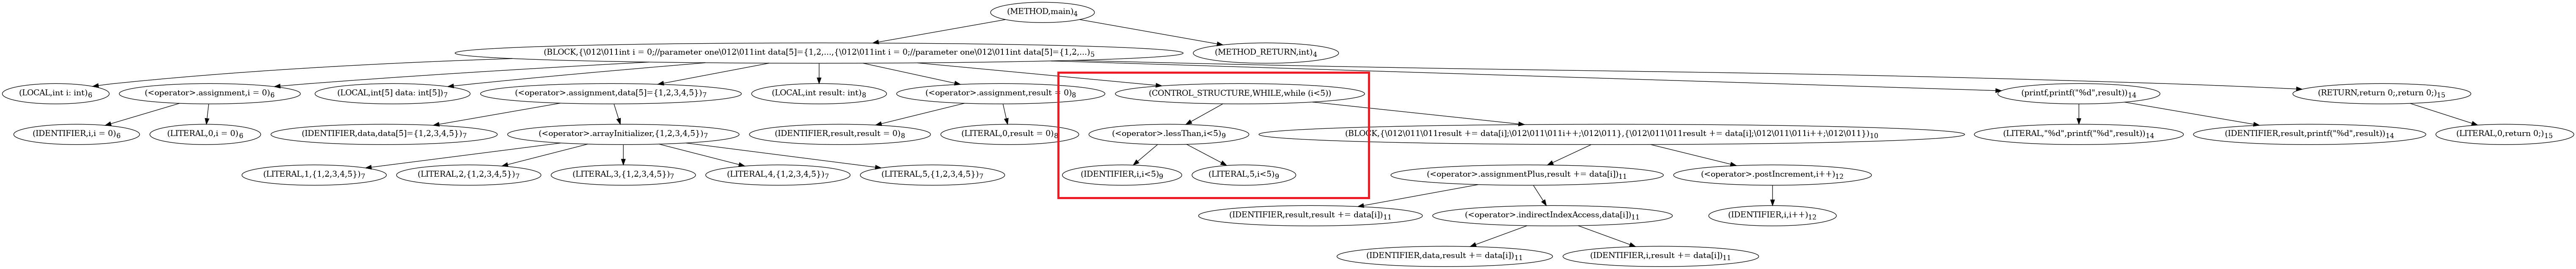
\includegraphics[width=0.3\textwidth]{figures/ast2}
      \label{fig:ast2} %引用标签
  }
  \subfigure[代码片段3对应的AST]{ %第三张子图
      \centering    %子图居中
      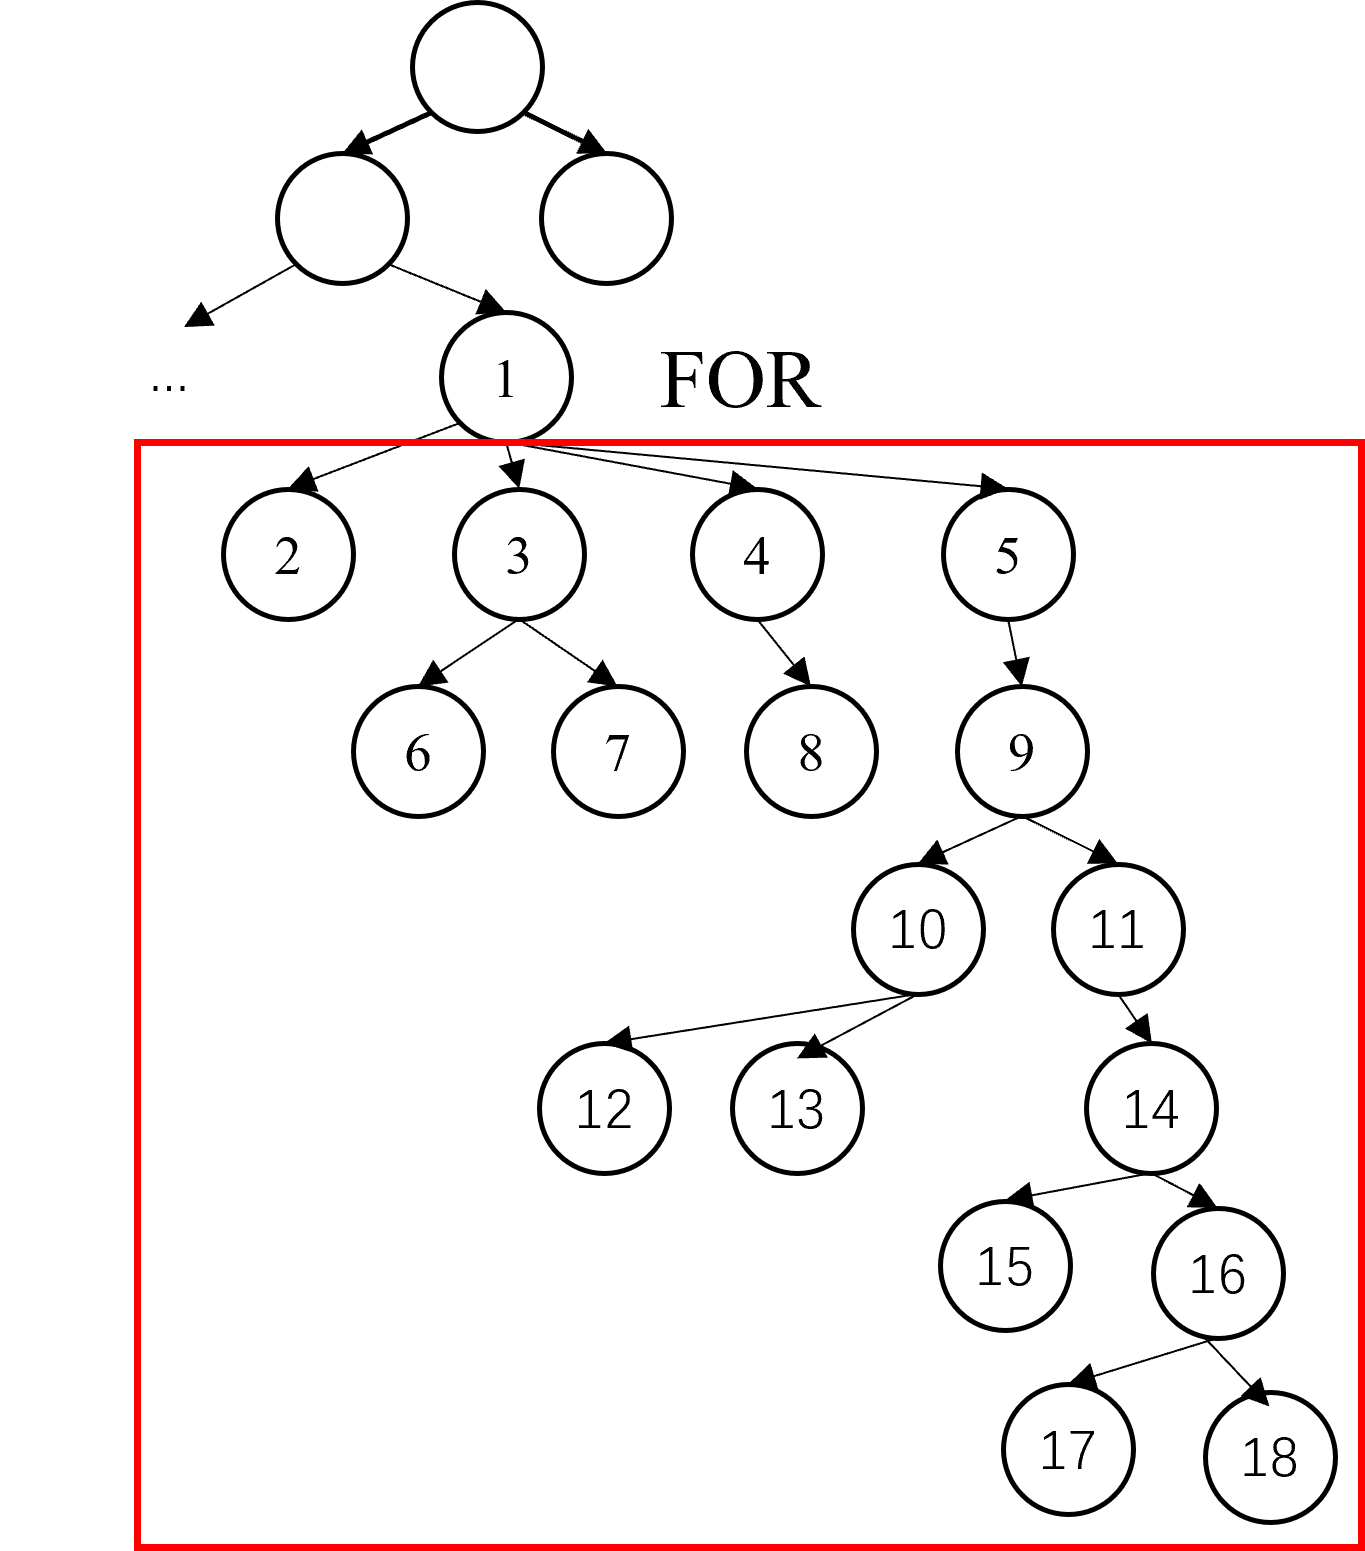
\includegraphics[width=0.25\textwidth]{figures/ast3}
      \label{fig:ast3} %引用标签
  }
  \caption{示例源代码对应的抽象语法树}    %大图名称
  \label{fig:astcode}    %图片引用标记
\end{figure}

接下来,本章提出的基于子树划分的抽象语法树表征学习方法的实现如图\ref{fig:ast}所示。该方法的输入是一对代码片段$C_{a},C_{b}$对应的抽象语法树,表示为$AST_{a},AST_{b}$,输出是$C_{a},C_{b}$对应的结构特征向量 $V_{a}^{AST},V_{b}^{AST}$,整体采用Siamese架构,两个子网络共享权值,从下到上,主要包括子树划分、子树表征、树表征三个阶段。

\begin{figure}[H]
  \centering
  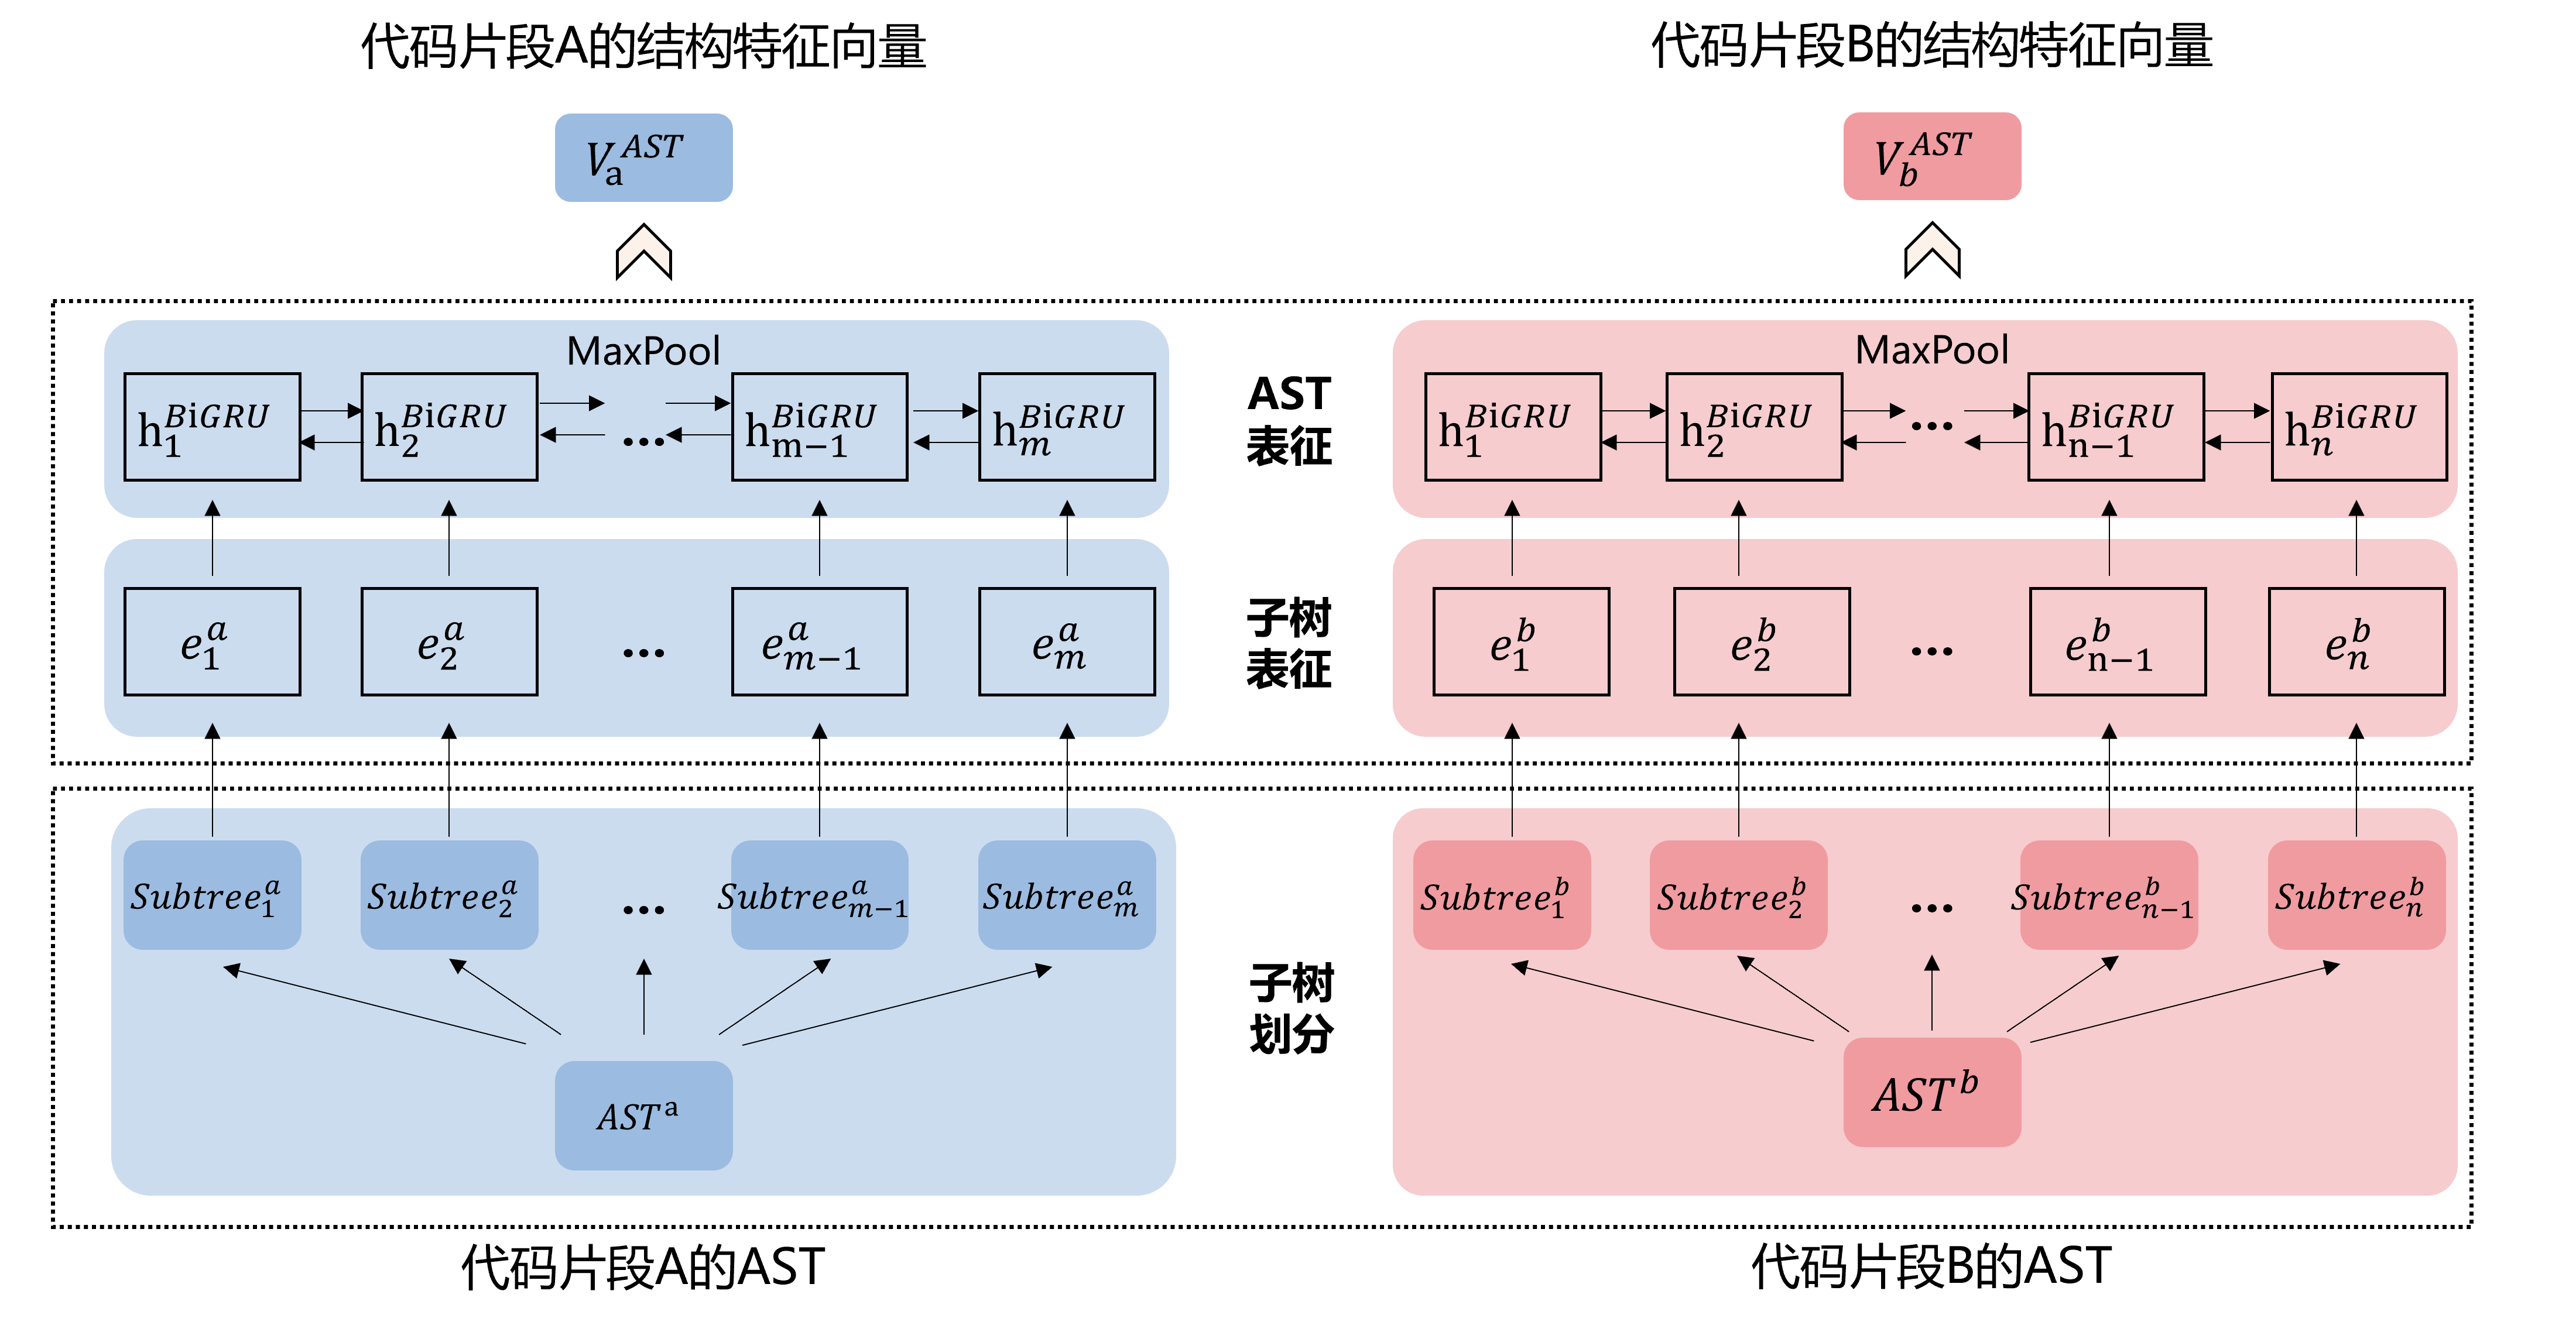
\includegraphics[width=0.9\textwidth]{figures/ast}
  \caption{基于子树划分的抽象语法树表征学习方法实现}\label{fig:ast}
\end{figure}

具体来说,在子树划分阶段,对于代码片段$C_{a}$,经过代码分析工具Joern生成得到抽象语法树$AST_{a}$,通过子树划分算法,可以得到子树序列,用$\left(SubTree_{1}^{a},SubTree_{2}^{a},\ldots,\notag \right.\\\left.SubTree_{1}^{m}\right)$表示,$m$是子树序列的长度。其子树划分过程可以表示为公式\ref{e4.8}:

\begin{equation}\label{e4.8}
  \begin{split}
    \left(SubTree_{1}^{a},SubTree_{2}^{a},\ldots,SubTree_{m}^{a}\right) = split\_AST \left(AST_{a}\right)
  \end{split}
\end{equation}

经过子树划分后,代码片段$C_{a}$生成了子树序列$\left(SubTree_{1}^{a},SubTree_{2}^{a},\ldots,SubTree_{m}^{a}\right)$。使用同样的划分方法,可以得到代码片段$C_{b}$生成了子树序列$\left(SubTree_{1}^{b},SubTree_{2}^{b},\ldots,\notag \right.\\\left.SubTree_{n}^{b}\right)$,$n$是代码片段$C_b$对应的子树序列长度。

在树表征阶段,首先将代码片段的子树序列作为输入,使用基于树的卷积神经网络模型进行编码,得到每个子树对应的语句向量$\left( e_{1}^{a},e_{2}^{a},\ldots,e_{m}^{a}\right)$。然后,使用双向门控循环单元(BiGRU)来模拟语句的自然性,通过最大池化层将BiGRU的隐藏状态采样到单个固定长度的向量$V_{a}^{AST}$中,作为最终的抽象语法树表示,即结构特征向量。具体的处理过程如公式\ref{e4.9}
\begin{equation}\label{e4.9}
  \begin{split}
    h_{1}^{aBiGRU},h_{2}^{aBiGRU},\ldots,h_{n}^{aBiGRU} = BiGRU \left(e_{1}^{a},e_{2}^{a},\ldots,e_{m}^{a}\right) \\
    V_{a}^{AST} = MaxPool \left( h_{1}^{aBiGRU},h_{2}^{aBiGRU},\ldots,h_{n}^{aBiGRU} \right)
  \end{split}
\end{equation}

同样,可以使用相同的计算以子树序列$\left(SubTree_{1}^{b},SubTree_{2}^{b},\ldots,SubTree_{n}^{b}\right)$作为输入为代码片段$C_{b}$计算$V_{b}^{AST}$。


\section{实验验证}
\label{sec:ASTExperiment}
为了验证基于子树划分的抽象语法树表征学习方法的有效性,本节开展实验验证。首先,介绍了实验的具体设计,接着对子树划分、树表征模型进行消融实验。

\subsection{实验设计}
\label{subsec:ASTDesign}

本节使用与\ref{sec:TokenExperiment}节中同样的实验环境、数据集对基于子树划分的抽象语法树表征学习方法进行对比实验。本实验使用代码分析工具Joern获取数据集中代码片段的抽象语法树AST,然后使用基于树的卷积神经网络训练子树嵌入,并将嵌入向量大小设置为128。同样选取常用的精确率(Precision)、召回率(Recall)、F1值作为评估指标。

\subsection{实验结果}
\label{subsec:TokenResult}

(1)拆分AST粒度的实验结果

为了探究子树拆分对抽象语法树表征实验结果的影响,本文设计了三种不同的方法来处理AST。首先,将代码片段原始的完整抽象语法树视为一个特殊的子树,不进行拆分,用AST-Full表示,即粒度威威整棵树,完全不进行子树划分。其次,将AST的所有节点均提取为子树,用AST-Node表示,即粒度精确到每个节点。最后,根据子树划分块来处理抽象语法树,用AST-Block表示。本实验采取单一变量原则,仅修改AST拆分粒度,后续子树的编码采用相同的基于树的卷积神经网络,采用双向GRU处理整棵树的嵌入。具体实验结果如表\ref{tab:subtree}所示。


\begin{table}[htp] 
  \centering
  \caption{抽象语法树子树划分对实验结果的影响} 
  \label{tab:subtree}
  %\renewcommand{\arraystretch}{1.1}
  \begin{tabular*}{0.9\textwidth}{@{\extracolsep{\fill}}cccc}
  \toprule
  \multirow{2}{*}{AST划分粒度} & \multicolumn{3}{c}{POJ104} \\
  \cmidrule{2-4} 
   & 准确率P(\%) & 召回率R(\%) & F1值(\%)  \\  
  \midrule
    AST-Full			&85.74	  &87.72		   &86.70 \\
    AST-Node      &89.78	  &87.88		   &88.82 \\
    AST-Block			&92.75	  &87.62		   &90.11 \\
  \bottomrule
  \end{tabular*}
\end{table}

从表\ref{tab:subtree}可以看出,AST-Block优于AST-Full和AST-Node。探究其原因,AST-Full未进行子树划分,因此抽象语法树通常规模过大,在模型训练过程中容易造成梯度消失,权重无法及时更新,同时无法提取子树粒度的代码信息,从而导致代码检测的效果最差。而AST-Node将树的每一个节点都设为子树,导致基于树卷积的神经网络输入规模过大,影响检测效率。AST-Block很好地平衡了子树大小和句法信息的丰富性,其F1值达到了90.11。因此,得出以下结论:本章提出的子树划分算法对代码克隆的检测具有一定的优势。

(2)树表征模型实验结果

为了探究树表征模型GRU对实验结果的影响,本文在子树划分的基础上,将GRU模型与LSTM模型进行对比,结果如表\ref{tab:tree2}所示。

其中,GRU、LSTM均基于Pytorch1.10实现,其参数设置为:\ding{172} 子树划分:采用AST-Block的划分方法。\ding{173} 子树的表征均采用基于树的卷积神经网络,整树的表征模型的隐藏层维度设置为128,模型使用二元交叉熵作为损失函数,使用Adam优化器来训练模型参数,其中,学习率Learning\_rate设置为0.001,Dropout为0.5,训练批次Epochs为50,批处理大小Batch\_size为32,阈值Threshold为0.5,当相似度超过0.5,输入的代码对被判定为真克隆对,否则被判定为假克隆对。参数的确定是通过多次调试后选择最优参数作为最后的结果。

\begin{table}[htp]  
  \centering  
  \caption{树表征模型对实验结果的影响}   
  \label{tab:tree2}
  %\renewcommand{\arraystretch}{1.1}  
  \begin{tabular*}{0.9\textwidth}{@{\extracolsep{\fill}}cccc}  
  \toprule  
  表征模型 & 准确率P(\%) & 召回率R(\%) & F1值(\%)  \\  
  \midrule
  LSTM			  & 92.21	  & 83.52	 & 87.65		\\  
  GRU		      & 92.75	  & 87.62	 & 90.11 \\ 
  \bottomrule  
  \end{tabular*}  
\end{table}

基于对表\ref{tab:tree2}数据的分析,可以得到以下结论:(1)在对整树进行表征的过程中,LSTM模型的整体表现略差于GRU,准确率整体相当,两者均可以解决传统循环神经网络中存在的梯度消失问题。(2)LSTM模型的召回率比GRU低4.10\%。深究其原因,可能是因为LSTM由于单元内包含三个门,计算机制复杂,所以影响其召回率,而GRU模型结构相对简单,只有两个门,参数数量较少,模型收敛速度更快,计算效率更高。因此,在树维度的代码表征模型选取上,本文更倾向于GRU。


(3)树表征可视化

为了更直观地展示本文提出的基于子树划分的抽象语法树表征学习方法的有效性,本实验同样使用t-SNE技术将高维结构特征向量可视化,按照预先设定的参数,树表征学习后生成的张量维度是128,采用t-SNE技术将128维的张量转换为2维,得到的样本表征结果如图\ref{fig:origintwo}所示。

\begin{figure}[H] 
  \centering  %居中
  \subfigure[初始向量可视化]{   %第一张子图
      \centering    %子图居中
      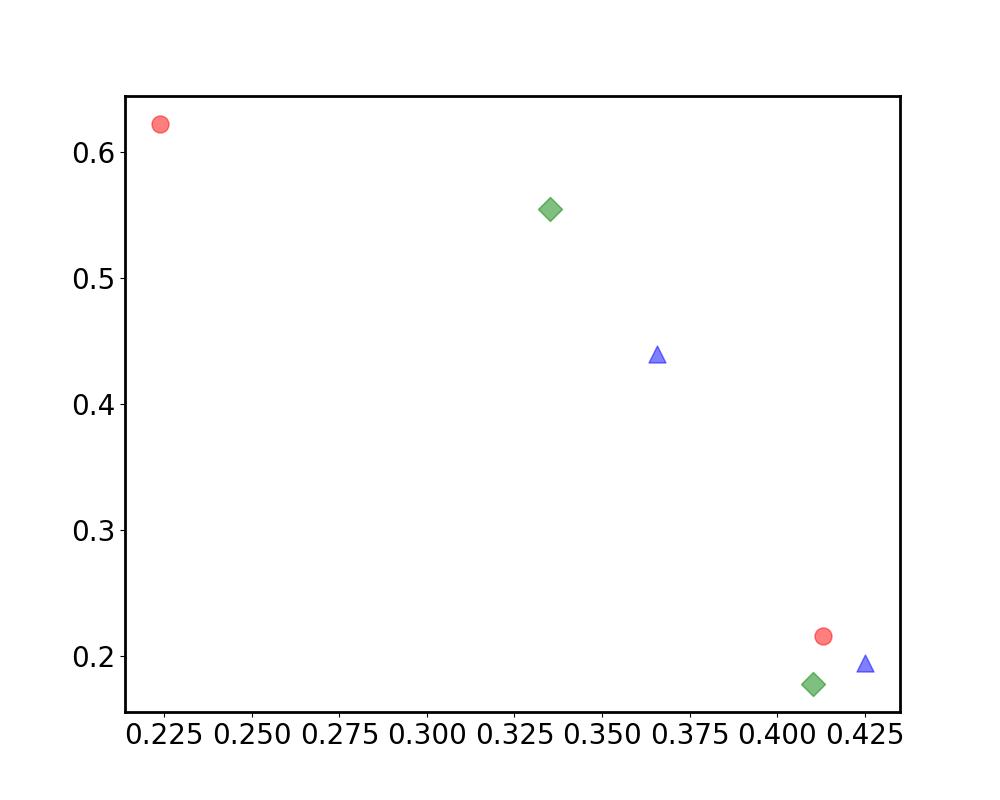
\includegraphics[width=0.45\textwidth]{figures/origin.png} 
      \label{fig:origint} %引用标签
  }
  \subfigure[结构特征向量可视化]{ %第二张子图
      \centering    %子图居中
      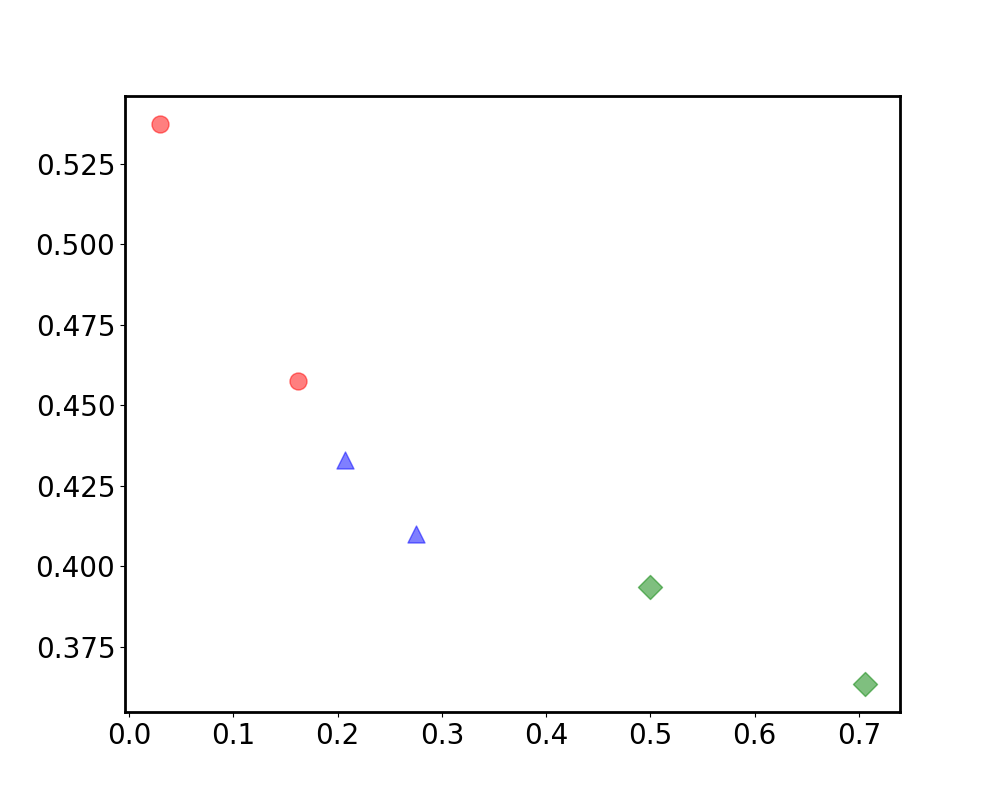
\includegraphics[width=0.45\textwidth]{figures/origin2.png}
      \label{fig:origin2} %引用标签
  }
  \caption{t-SNE技术降维后的结构特征向量可视化结果}    %大图名称
  \label{fig:origintwo}    %图片引用标记
\end{figure}

如图\ref{fig:origintwo}所示,\ref{fig:origint}和\ref{subsec:TokenResult}可视化实验中采用的代码片段相同,而\ref{fig:origin2}中,向量空间的所有点是代码片段通过树表征学习后得到的结构特征向量可视化结果。可以看到互为真克隆对的代码片段在经过树表征模型训练后相互聚。并且,与Token维度表征后的属性特征向量可视化结果\ref{fig:origin1}相比,树维度的可视化结果更优秀,说明树维度相比于Token维度包含了更多代码信息,模型有效地学习到了更有效的代码表征。


\section{本章小结}
\label{sec:Summary4}
本章主要对RLCCD中基于子树划分的抽象语法树表征学习方法的设计与实现进行详细阐述。首先介绍了抽象语法树维度的研究动机,其次介绍了抽象语法树表征学习的方法设计,具体论述了其整体框架、子树划分、树表征学习,接着开展实验验证,结果表明了此方法的有效性和模型的准确性。




\chapter{基于图过滤的程序依赖图表征学习}
\label{chap:PDG}
本章主要对本文提出的基于图过滤的程序依赖图表征学习方法进行详细介绍,首先介绍其基本思想,其次阐述其具体方法设计与实现,最后进行实验验证。

\section{研究动机}
\label{sec:PDGMotivation}

程序依赖图PDG是代码的一种图形表示,所含结构信息最多,能够表示程序的控制依赖,数据依赖等关系,是一种带有标记的有向多重图。程序依赖图PDG结点代表语句,边代表依赖关系,依赖关系包括数据依赖和控制依赖。基于图的代码表征方法首先使用代码分析工具构建包含代码语法结构、调用关系、数据流等信息的程序依赖图,然后通过子图匹配的方法,将PDG图中的控制流和数据流编码为一个紧凑的语义特征矩阵,其中每个元素都是一个高维的稀疏二值特征向量。通过将代码表示为图的形式使得模型能够更好地理解代码中不同部分之间的依赖关系,更适合研究代码内的丰富语义信息。

基于图的代码表征方法存在两种主要限制:

(1)规模开销较高:基于图的表征学习方法通常需要构建代码的结构图或控制流图作为分析的基础,对于具有复杂控制流或数据流的代码片段,构建准确的图表示是一个不小的挑战。特别地,当代码片段中具有循环、递归或异常处理机制时,图的构建过程更加困难。这些复杂结构不仅增加图构建的复杂性,还有可能导致图表示的精度下降;即使在成功生成图之后,图表征学习方法的计算成本也很高。例如,对图进行子图同构等操作时,往往需要借助复杂的图算法来实现,并将生成的程序依赖图两两匹配,对于包含$n$个代码片段的数据集,需要进行$n^2$次匹配检测。而其中包含大量无用的匹配,会浪费大量的时间和计算资源。这些算法不仅计算成本大,而且随着代码库规模的扩大,处理时间也会显著增加,导致开销高。

(2)对代码修改的敏感性:在实际开发过程中,代码通常会经过各种微小的更改,例如变量名更改、代码格式化、添加或删除注释等,这些修改可能会导致图的表示发生显著变化。具体来说,当代码中的变量名被更改时,图的节点和边可能会受到影响,因为变量名通常作为图中的一个重要特征被考虑在内。同样,代码格式的调整,如缩进、换行或空格的变化,虽然不影响代码的逻辑功能,但也可能导致图的拓扑结构发生变化。此外,添加或删除注释虽然对代码的执行没有影响,但在构建代码图时,这些注释也可能被当作图的一部分,从而影响到图的表示。因此,基于图的克隆检测方法可能无法准确地检测出这些轻微修改过的克隆代码。更进一步,随着代码库的不断增长和变化,基于图的克隆检测方法可能需要不断地更新和调整以适应新的代码结构。这意味着方法的实现和维护成本可能会相对较高,因为开发者需要定期更新和调整方法以适应代码的变化。这种持续的更新和调整不仅增加了工作负担,还可能影响到方法的长期有效性。

因此,针对上述问题,本文提出了一种基于图过滤的程序依赖图表征学习方法,该方法通过预处理图过滤,减少候选PDG对集合的规模。

\section{PDG表征方法方法设计}
\label{sec:PDG}
本节将介绍基于图过滤的程序依赖图表征学习方法设计与实现,首先介绍该方法的整体框架,并从图过滤、程旭依赖图表征学习两方面介绍具体设计。 

\subsection{框架概述}
\label{subsec:PDGOverview}
本文提出的基于图过滤的程序依赖图表征学习方法整体框架如图\ref{fig:pdgframework}所示。该框架的输入是代码片段对应的程序依赖图,输出是对应的语义特征向量,主要包括图过滤、图表征两个阶段。

\begin{figure}[H]
  \centering
  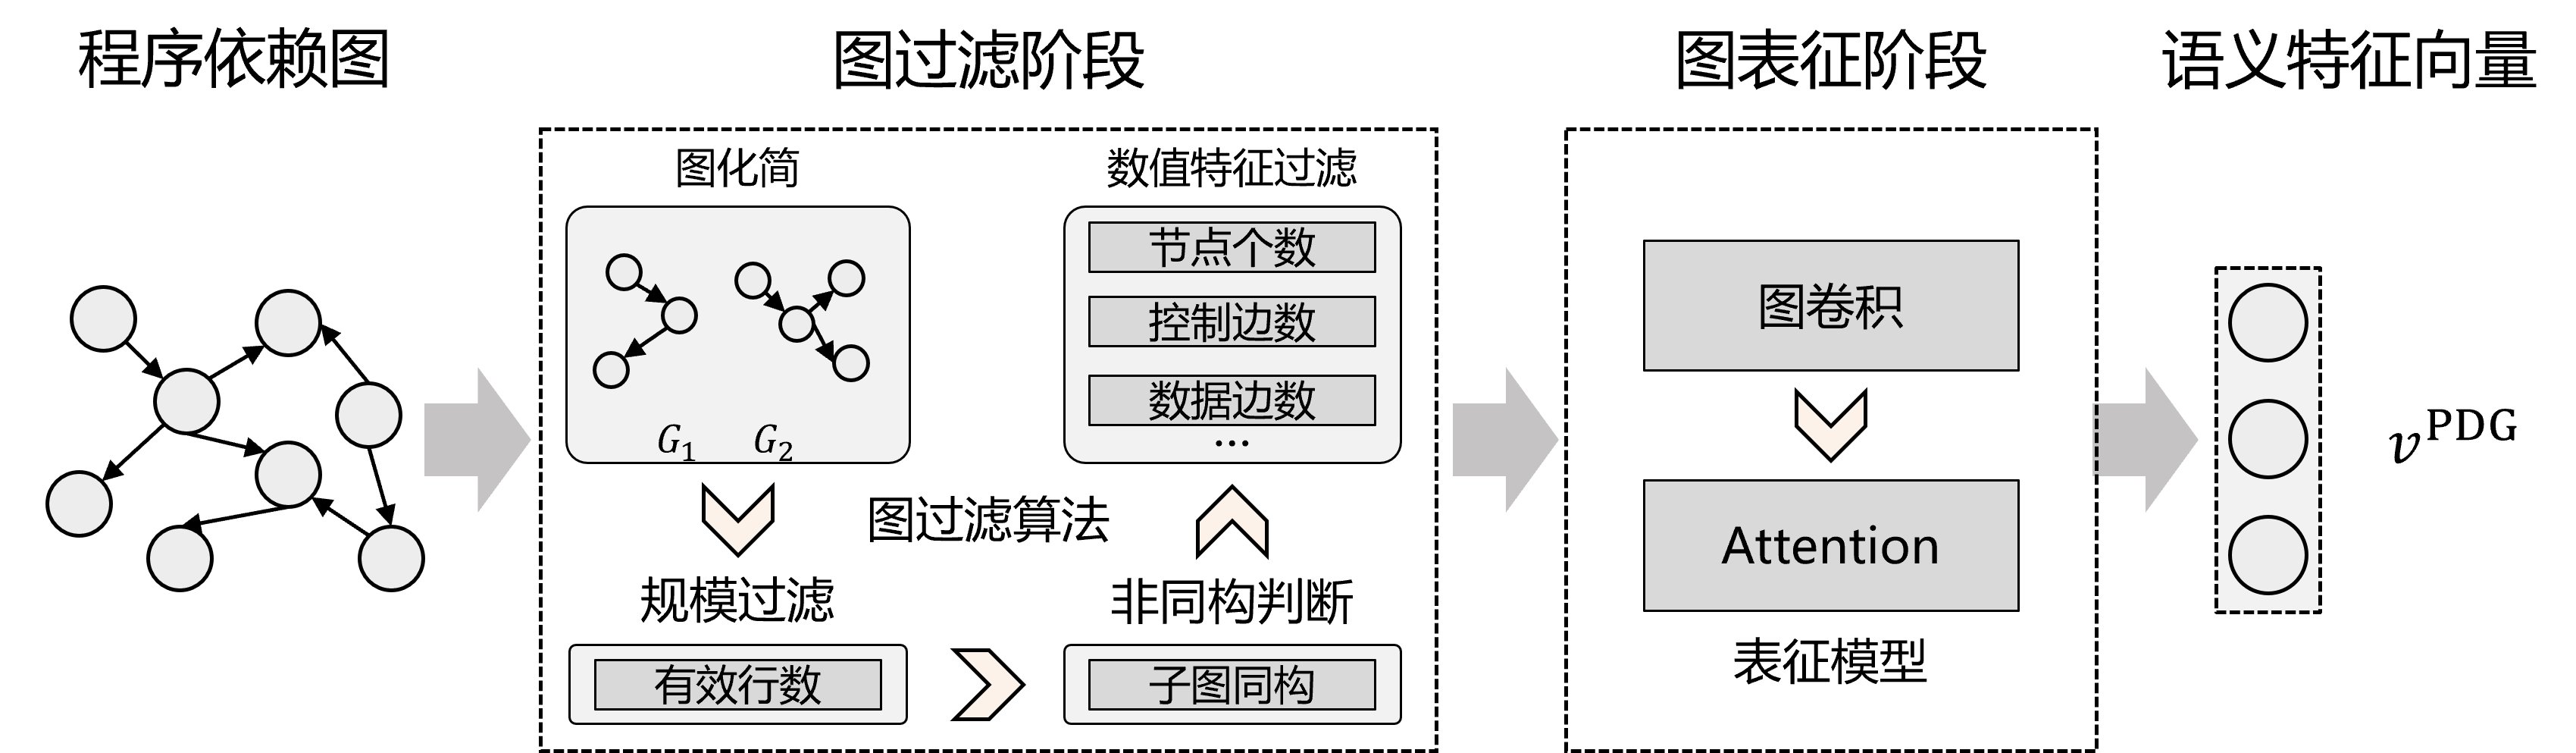
\includegraphics[width=0.95\textwidth]{figures/pdgframework.png}
  \caption{基于图过滤的程序依赖图表征学习框架}\label{fig:pdgframework}
\end{figure}

首先,图过滤阶段以代码片段对应的程序依赖图作为训练数据,设计一个基于候选程序依赖图对的图过滤算法,通过减少候选图对的规模,提高后续模型的训练能力。需要注意的是,为了更好地减少图规模,本文设计了一些有效的过滤策略,通过对PDG的边进行约简、对PDG对集合进行过滤的方式,只保留克隆可能性较大地候选PDG对,从而有效地加速检测过程,减少后续模型输入规模。

其次,图代码表征阶段以过滤后的程序依赖图作为训练数据,构建一个图表征模型。该模型的输入是程序依赖图,输出为一个固定长度的密集向量用来表示代码的语义特征。需要注意的是,本文选用的图卷积神经网络,主要包含两个部分:图卷积部分和自注意力机制部分,前者主要目的是通过在图上的卷积操作来捕捉节点的特征以及节点之间的关系。后者的主要目的是总结图节点特征,并将每个代码片段缩减为一个单一的密集向量。

在上述框架中,本文的创新点主要体现在图过滤阶段的图过滤算法、图代码表征阶段的模型设计两方面,下面将围绕这两个创新点来阐述本文的方法。


\subsection{图过滤设计}
\label{subsec:PDGPreModel}

本文使用代码分析工具Joern生成程序依赖图。其中,Joern通过静态分析源代码,生成关键的图结构信息,反映代码中的依赖关系和函数调用层次,同时Joern提供查询和可视化功能,用户可以通过命令将分析结果导出为多种格式,从而更好地理解代码的逻辑和流程。使用Joern工具,生成代码片段\ref{fig:code1}对应的程序依赖图,并导出DOT文件如\ref{fig:pdgshili1}所示,使用开源图形可视化工具Graphviz对DOT文件进行转化,可以得到如\ref{fig:pdgshili2}的图形。

\begin{figure}[H]
  \centering
  \subfigure[代码片段1对应的PDG DOT格式]{   %第一张子图
      \centering    %子图居中
      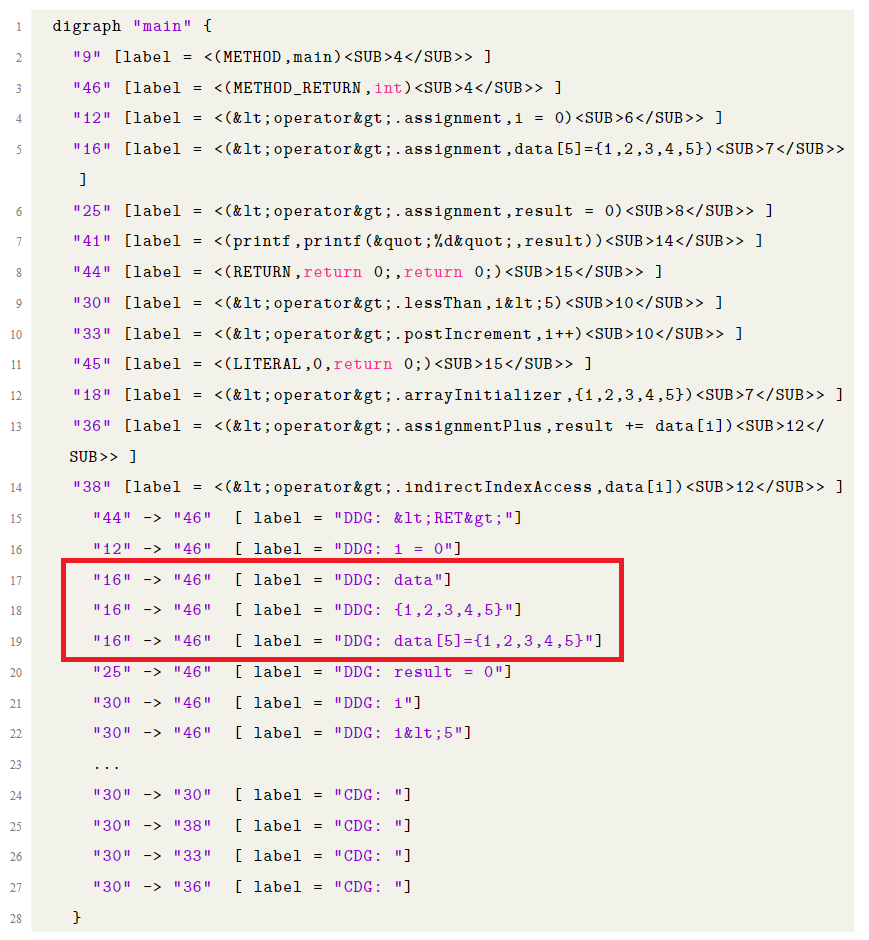
\includegraphics[width=0.4\textwidth]{figures/pdgshili}  
      \label{fig:pdgshili1} %引用标签
  }
  \subfigure[代码片段1对应的PDG可视化]{ %第二张子图
      \centering    %子图居中
      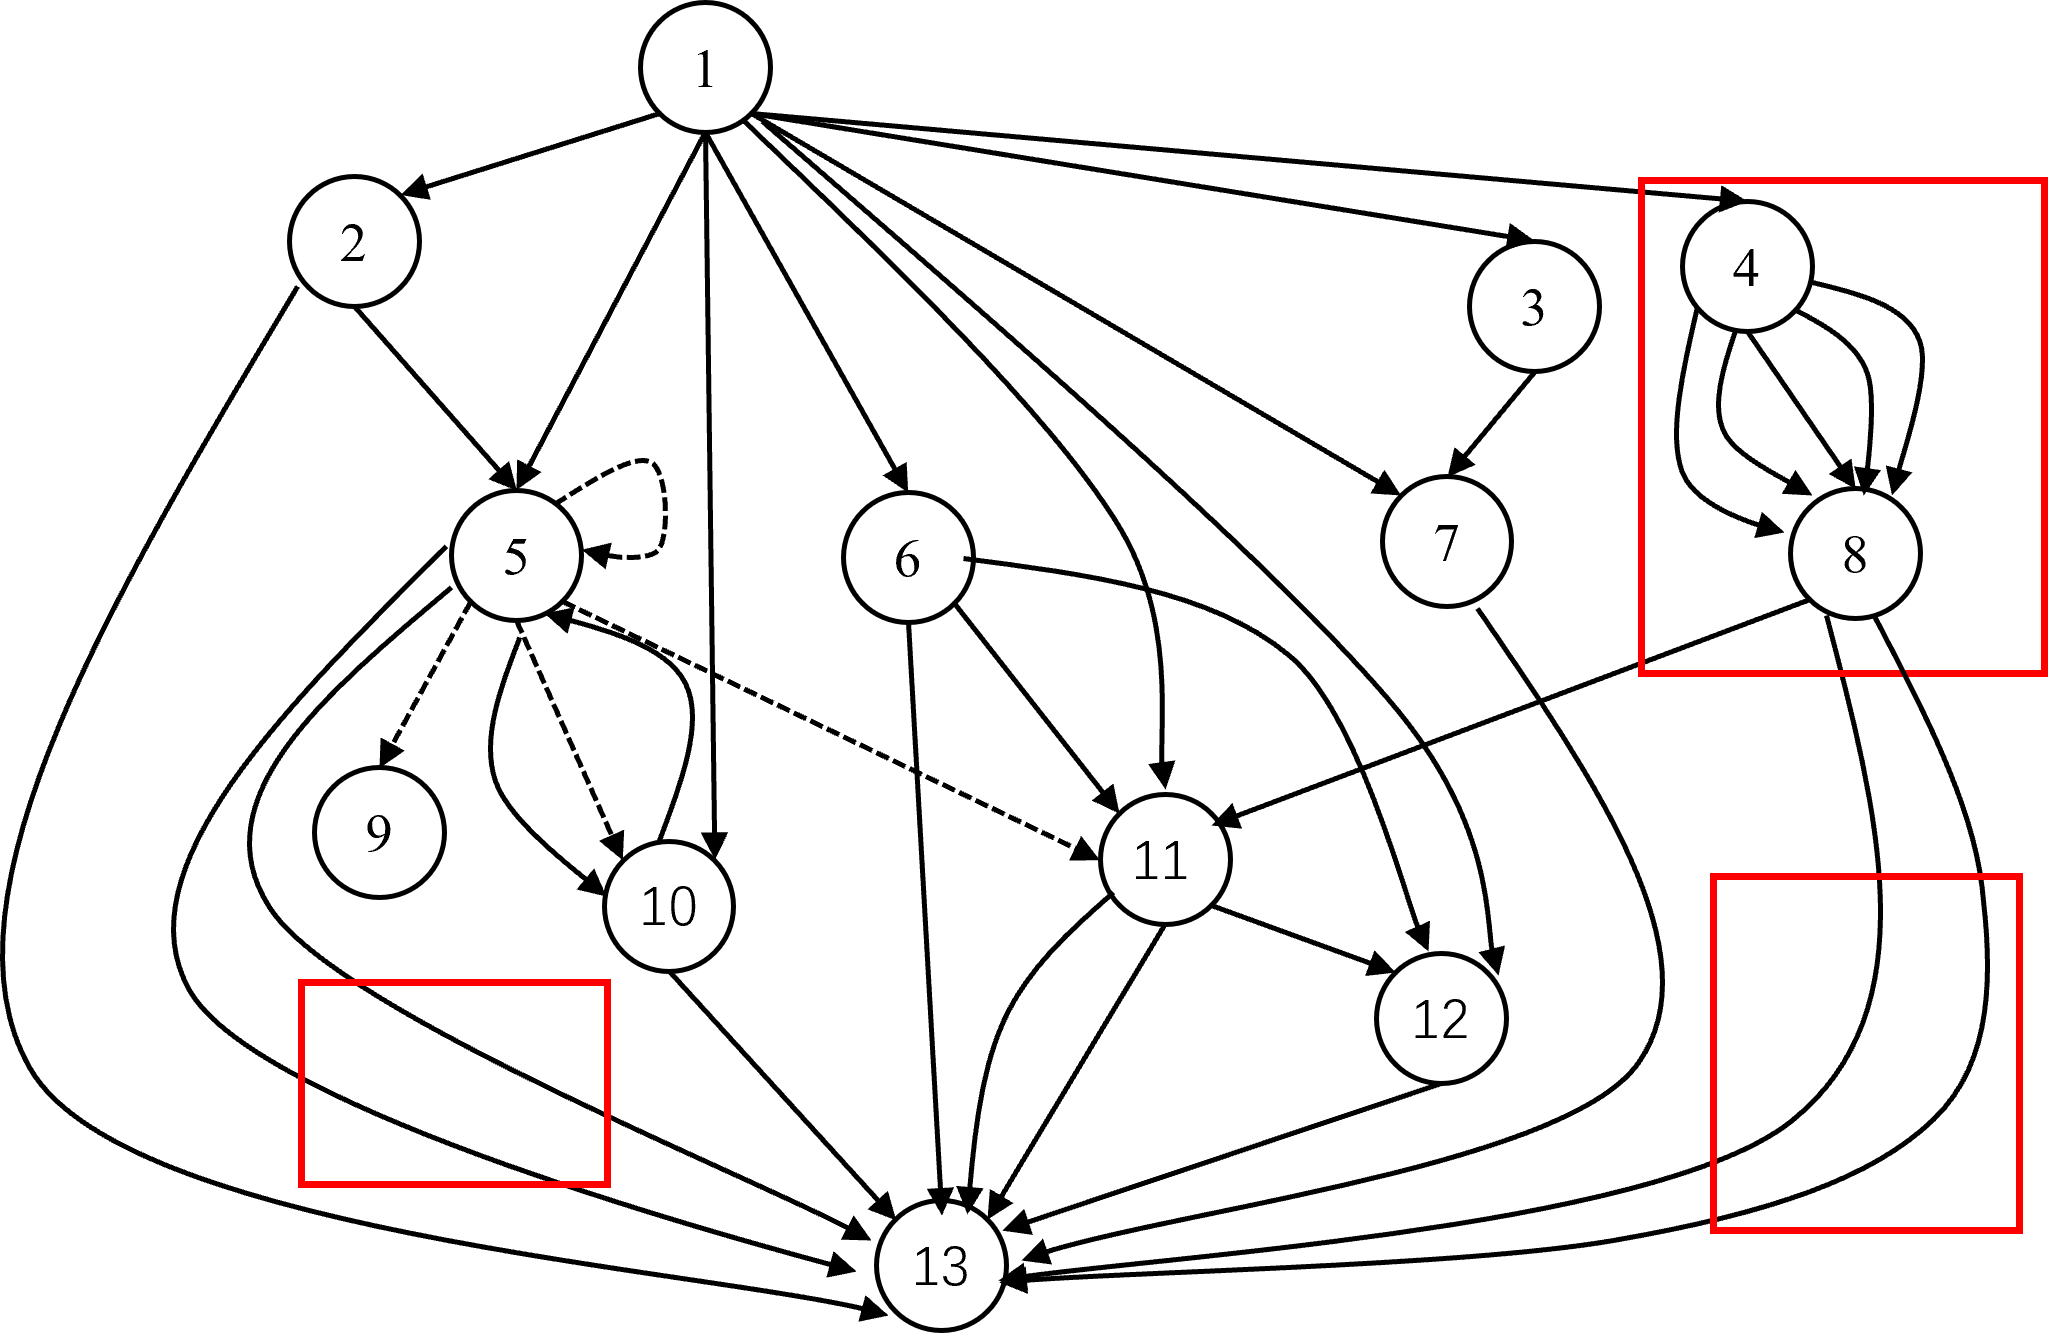
\includegraphics[width=0.5\textwidth]{figures/pdgshili2}
      \label{fig:pdgshili2} %引用标签
  }
  \caption{程序依赖图DOT文件示例}
  \label{fig:pdgshili}
\end{figure}
% \lstset{language=C}
% \begin{lstlisting}
%   digraph "main" {  
%     "9" [label = <(METHOD,main)<SUB>4</SUB>> ]
%     "46" [label = <(METHOD_RETURN,int)<SUB>4</SUB>> ]
%     "12" [label = <(&lt;operator&gt;.assignment,i = 0)<SUB>6</SUB>> ]
%     "16" [label = <(&lt;operator&gt;.assignment,data[5]={1,2,3,4,5})<SUB>7</SUB>> ]
%     "25" [label = <(&lt;operator&gt;.assignment,result = 0)<SUB>8</SUB>> ]
%     "41" [label = <(printf,printf(&quot;%d&quot;,result))<SUB>14</SUB>> ]
%     "44" [label = <(RETURN,return 0;,return 0;)<SUB>15</SUB>> ]
%     "30" [label = <(&lt;operator&gt;.lessThan,i&lt;5)<SUB>10</SUB>> ]
%     "33" [label = <(&lt;operator&gt;.postIncrement,i++)<SUB>10</SUB>> ]
%     "45" [label = <(LITERAL,0,return 0;)<SUB>15</SUB>> ]
%     "18" [label = <(&lt;operator&gt;.arrayInitializer,{1,2,3,4,5})<SUB>7</SUB>> ]
%     "36" [label = <(&lt;operator&gt;.assignmentPlus,result += data[i])<SUB>12</SUB>> ]
%     "38" [label = <(&lt;operator&gt;.indirectIndexAccess,data[i])<SUB>12</SUB>> ]
%       "44" -> "46"  [ label = "DDG: &lt;RET&gt;"] 
%       "12" -> "46"  [ label = "DDG: i = 0"] 
%       "16" -> "46"  [ label = "DDG: data"] 
%       "16" -> "46"  [ label = "DDG: {1,2,3,4,5}"] 
%       "16" -> "46"  [ label = "DDG: data[5]={1,2,3,4,5}"] 
%       "25" -> "46"  [ label = "DDG: result = 0"] 
%       "30" -> "46"  [ label = "DDG: i"] 
%       "30" -> "46"  [ label = "DDG: i&lt;5"] 
%       ...
%       "30" -> "30"  [ label = "CDG: "] 
%       "30" -> "38"  [ label = "CDG: "] 
%       "30" -> "33"  [ label = "CDG: "] 
%       "30" -> "36"  [ label = "CDG: "] 
%     }
% \end{lstlisting}

%\notag \right.\\\left.

分析上图\ref{fig:pdgshili1},程序依赖图DOT文件的描述包含两个部分:使用\textquotedbl number \textquotedbl [label =  <\(function,name\)> ]来描述PDG点的特征,包括节点编号、节点的标签,其中标签内还包括源代码语句中的变量名称、变量属性等信息。使用\textquotedbl number \textquotedbl $\to$ \textquotedbl number \textquotedbl [label = \textquotedbl CDG/DDG:data \textquotedbl ]来描述PDG边的特征,包括边的起始点编号、边的终点标号、边代表的依赖关系(控制依赖用CDG表示、数据依赖用DDG表示)。使用开源图形可视化工具Graphviz得到的图\ref{fig:pdgshili2}中包含13个顶点,用实线箭头表示数据依赖边,虚线箭头表示控制依赖边。通过DOT描述语言存储生成的PDG能够很好的表现出代码片段的语法信息,表示出不同的节点和边的各种特征和属性,为下一步的过滤算法打好基础。

如果代码片段功能复杂,那么对应的程序依赖图规模也会很大,同时包含很多冗余边。例如上图\ref{fig:pdgshili2}中红框中的边,它们起始节点、终止节点均相同。右上角的红框对应\ref{fig:pdgshili1}中的data数组,数组内包含5个元素,对应含有5条边。实际上,这些边只有数值不同,属性相同,因此需要进行适当的优化来使得程序程序依赖图的结构精简,又不会丢失语义信息。

针对上述问题,本文设计了一种基于候选图对集合的图过滤算法,算法的伪代码如\ref{alg3}所示。该算法有多个输入:候选程序依赖图集合$G$、PDG有效行数阈值$L$、程序依赖图对规模比率$T$,输出为:经过过滤后的PDG对集合$R$,初该算法分为四个步骤:PDG图结构化简、规模过滤、非同构判断、数值特征过滤,每个步骤的作用如下:

\begin{algorithm}[ht]  
	\renewcommand{\algorithmicrequire}{\textbf{Input:}}
	\renewcommand{\algorithmicensure}{\textbf{Output:}}
	\caption{Graph filter algorithm $\left(filter\_PDG\right)$}  
	\label{alg3}
	\begin{algorithmic}[1]
    \Require PDG pairs:$G$
    \Require The threshold:$L$
    \Require The threshold of PDG pair's scale ratio:$T$
    \Require The threshold of CV's string numberical similarity:$G_s$
		\Ensure Candidate PDG pairs:$R$
    \State initialization
		\For{each PDG paris $G_1,G_2$  $in$ $G$}
      \State deleteSelfLoops($G_1$)
      \State deleteSelfLoops($G_2$) \Comment{step1:PDG图结构化简}
      \If {sizeof($G_1$) < L or sizeof($G_2$) < L}
        \State PDG pair($G_1,G_2$) is filtered \Comment{step2:规模过滤}
      \Else
        \If {min($G_1,G_2$) / max($G_1,G_2$) < T}
          \If{there is subgraph between ($G_1,G_2$ )} \Comment{step3:非同构判断}
            \State R $\leftarrow$ R $\cup \left(G_1,G_2\right)$ 
          \Else
            \State PDG pair($G_1,G_2$ ) is filtered
          \EndIf
        \Else
          \If {number similarity of $G_1,G_2$ > $G_s$} \Comment{step4:数值特征过滤}
            \State R $\leftarrow$ R $\cup \left(G_1,G_2\right)$
          \Else
            \State PDG pair($G_1,G_2$ ) is filtered
          \EndIf
        \EndIf
      \EndIf 
    \EndFor \\
    \Return $R$
	\end{algorithmic}
\end{algorithm}

(1)PDG图结构化简:首先对候选程序依赖图集合中的图进行化简,对起始节点、终止节点均相同的边进行化简,仅保留一条边,从而减少图的大小以便后续图匹配操作。下图\ref{fig:pdgshili3}是化简后的结果。

\begin{figure}[H]
  \centering
  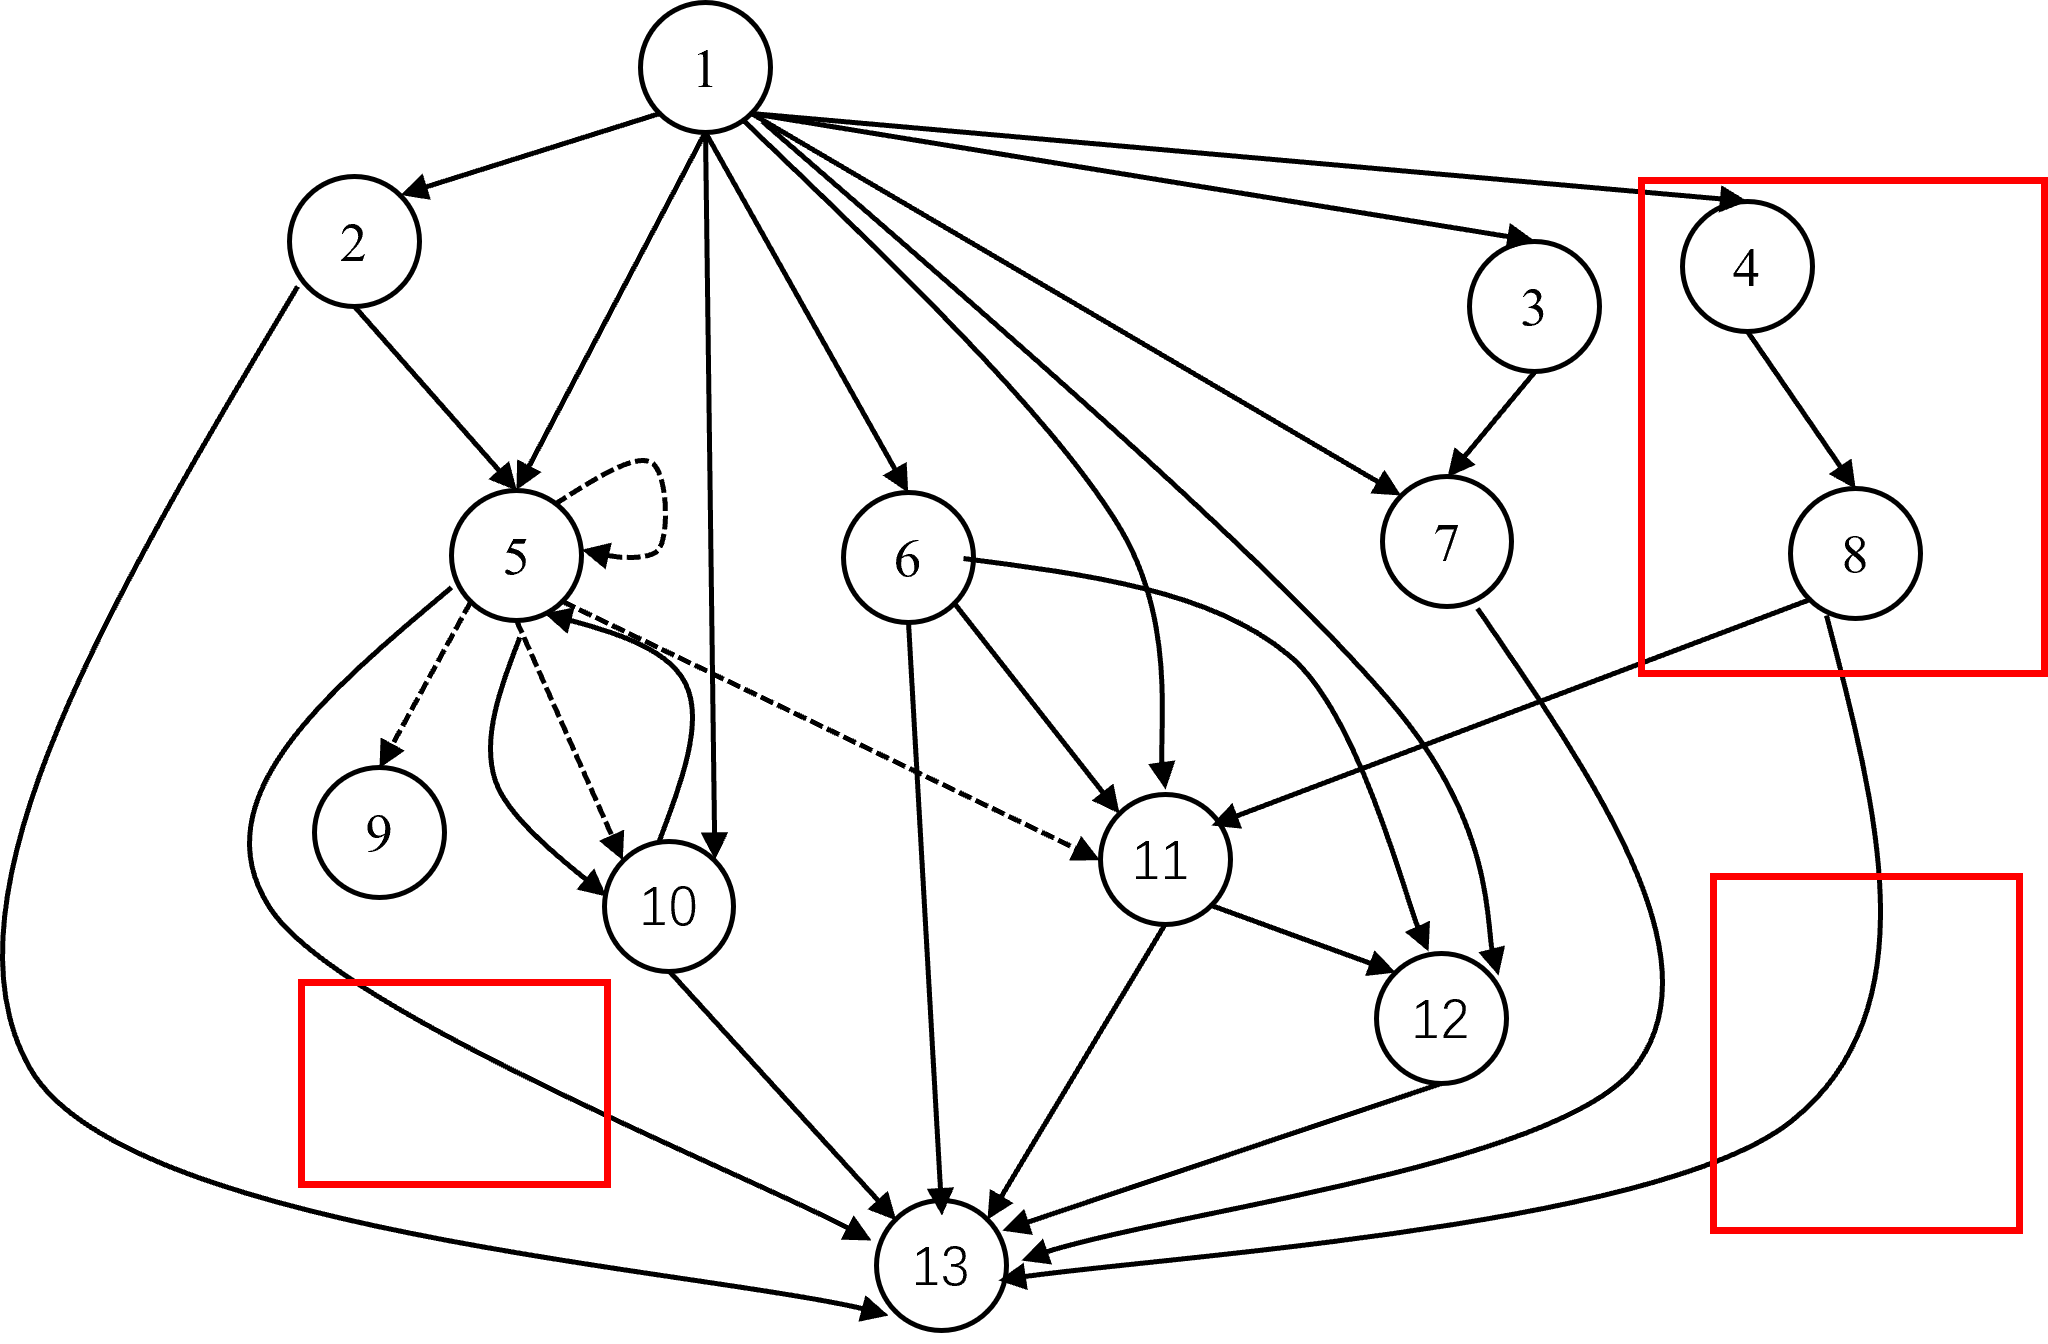
\includegraphics[width=0.55\textwidth]{figures/pdgshili3.png}
  \caption{代码片段1经过图结构化简后的图}\label{fig:pdgshili3}
\end{figure}

(2)规模过滤:其次对图的规模进行判断,针对代码克隆检测,有研究证明,有效行数小于6行的克隆程序本身并没有任何意义,并且会被绝大多数的代码克隆检测工具忽略.因为小于6行有效行的函数多为空函数,没有太大的参考意义。因此,本文也设置一个阈值,如果PDG1和PDG2中有任意一个PDG的有效行数小于阈值,那么就需要过滤掉这对PDG。

(3)非同构判断:接着对PDG对中是否存在子图同构进行判断。假设一对PDG对中,规模较大的图为$G_1$,规模较小的图为$G_2$,根据子图同构的概念,只要$G_1$和$G_2$满足以下两个条件之一:
\begin{equation}\label{e5.1}
  \begin{split}
    max(O(G_1)) < max(O(G_2)) \\
    min(I(G_1)) < min(I(G_2))
  \end{split}
\end{equation}

那么这两个图就不可能存在子图同构关系。其中$O(G)$表示程序依赖图的节点出度,$I(G)$表示程序依赖图的节点入度。如果这对PDG不存在子图同构,但节点总数相差很大,那么就需要过滤掉这对PDG。

(4)数值特征过滤:最后通过收集PDG的简单特征来过滤掉明显不可能为克隆的PDG对。具体的,根据PDG的节点个数、控制边数、执行边数、数据边数、声明节点数、函数调用数、传入参数、传出参数等代表特征进行过滤,这些特征包含了代码一定的语义和语法信息。通过过滤掉差异很大的PDG对,从而减少候选PDG对集合的规模。


\subsection{程序依赖图表征学习设计}
\label{subsec:PDGModel}

(1)结构设计

为了提高程序依赖图维度代码表征能力,本文选取图卷积网络对上述得到程序依赖图进行建模。具体的模型设计如图\ref{fig:pdgmodel}所示。该模型主要包括输入层、多层卷积层、自注意力层、输出层。
\begin{figure}[H]
  \centering
  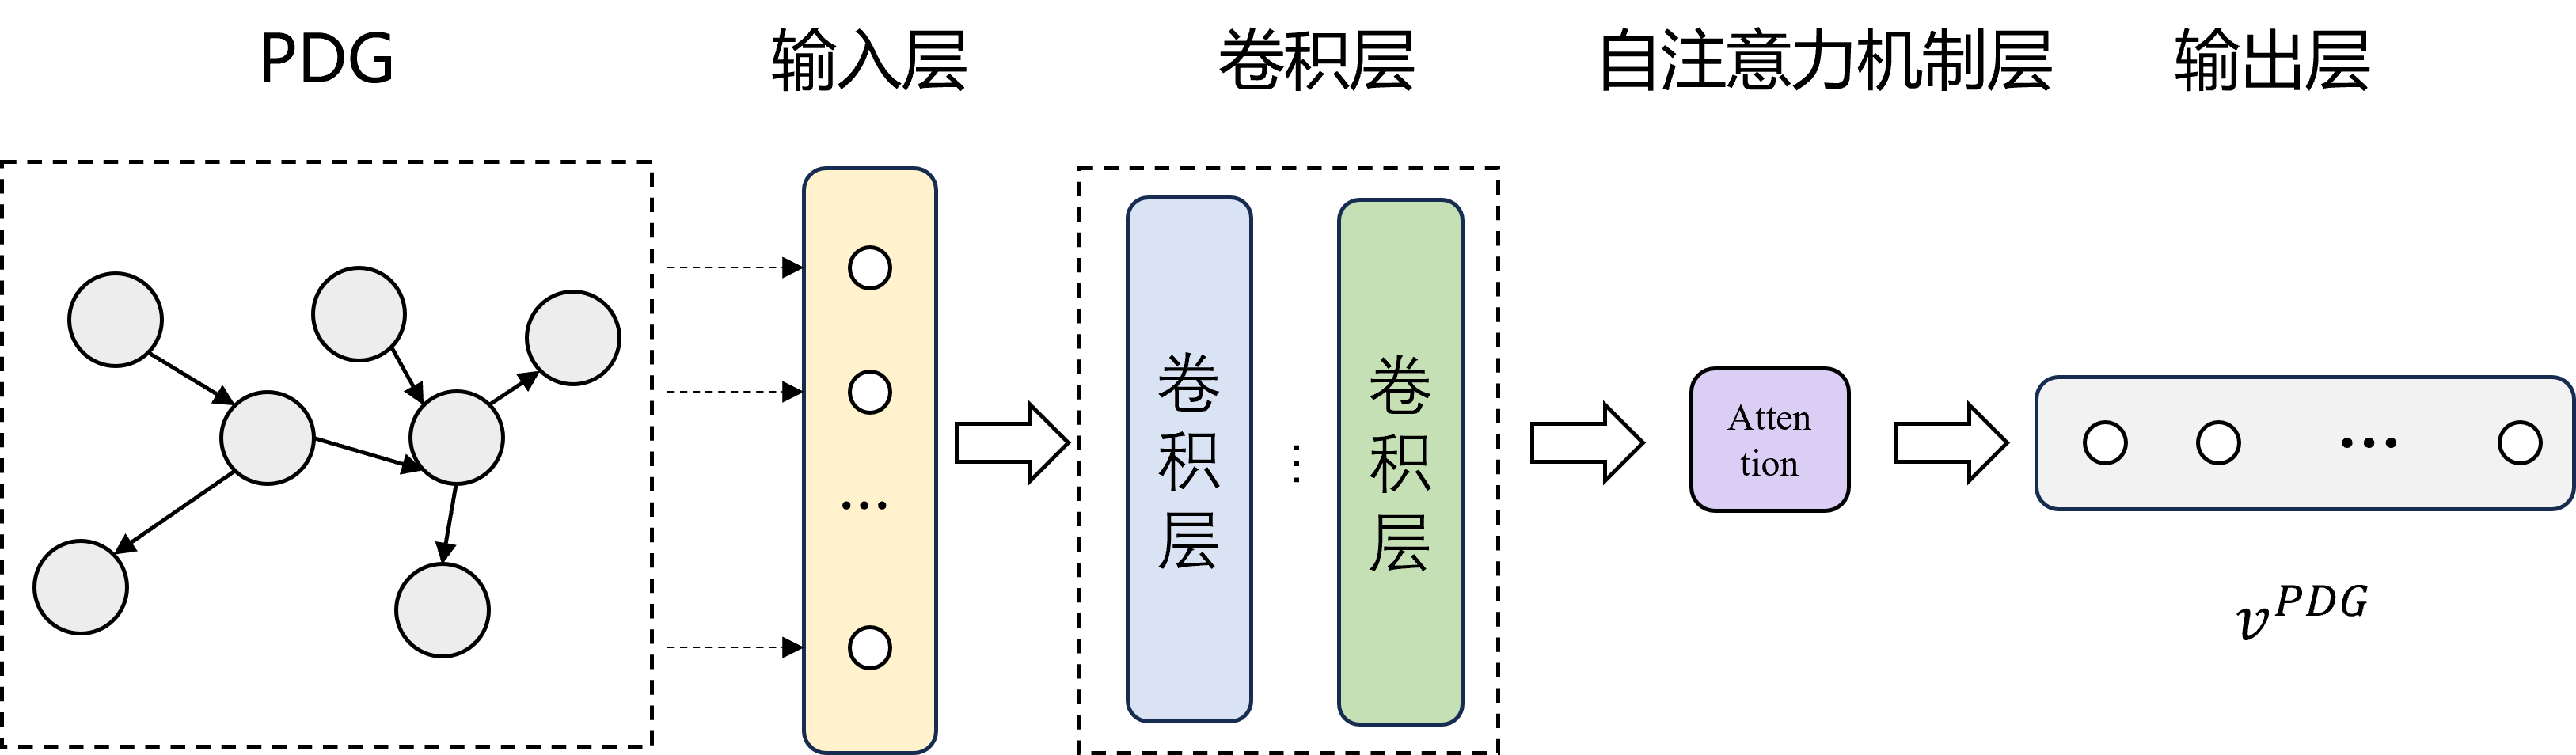
\includegraphics[width=0.85\textwidth]{figures/pdgmodel.png}
  \caption{程序依赖图表征模型设计}\label{fig:pdgmodel}
\end{figure}

\ding{172}输入层:输入层用于向模型输入训练数据,在本方法中模型的输入为经过过滤算法判断得到的程序依赖图。\ding{173}卷积层:由多层卷积层堆叠构成,通过卷积操作提取节点的特征,同时考虑到节点之间的关联。\ding{174}自注意力机制层:本层的主要目的是捕捉序列中的长距离依赖关系,通过直接计算任意两个位置的依赖关系,并将每个代码片段缩减为一个单一的密集向量。\ding{175}输出层:每个程序依赖图对应一个输出。

(2)模型选型

传统卷积神经网络中的卷积操作,是指利用滑动窗口在输入数据上平移,每次计算窗口内数据的有用特征,从而达到特征提取的目的。然而,这种操作只能处理图片、语言等结构规则的数据。现实中,像图结构这种不规则的数据普遍存在,其每个节点都拥有独特的邻接环境,无法通过传统CNN、RNN的方法计算。因此,有研究\cite{kipf2017semisupervised}提出图卷积神经网络。

在图结构中,每个节点都受到其邻居节点的影响,这种影响随着关系的紧密程度而变化,最终使节点达到稳定状态。图卷积神经网络(GCN)正是基于这样的思想,通过卷积操作来提取图中节点的特征。在GCN中,每个节点的特征表示不仅包含其自身的特征信息,还会考虑其所有邻居的特征信息,并通过学习得到的参数来更新。通过多层GCN的堆叠,可以逐步传播全局信息,实现对整个图的信息聚合和表示学习。相较于表真的CNN ,GCN能够很好地处理不规则和非欧氏空间的数据,因此在社交网络、化学分子结构、交通网络等领域有广泛应用。值得一提的是,图卷积操作具有置换不变性,即不依赖于节点的具体排序,这符合图数据的本质特性。

图卷积神经网络是一种特殊的前馈神经网络结构,为减少网络中参数个数,用卷积层来代替传统的全连接层,提高神经网络的训练效率,卷积神经网络可以提取信息最多的数据特征,生成一个固定大小的向量表示结构。这样的设计有助于深入挖掘数据的语法和语义信息,使得图卷积神经网络在代码克隆检测等任务中表现出色。

因此,本文选用图卷积神经网络来构建程序依赖图的表征学习模型,该模型通过聚合节点自身的信息和邻居节点的信息,实现节点表示的更新,通过多层图卷积堆叠,实现全图信息聚合,进而提升程序依赖图的特征提取能力。

首先给出GCN的符号定义:对于图$G=\left(V,E\right)$,其中$V$表示节点集,节点个数为$N$,对于每个节点$v_i \in V$,均有其特征向量$x_i$,节点的特征向量特征用矩阵$X \in R^{N×C}$表示,其中$C$表示每个特征向量的维度;$E$表示边的集合,如果节点$v_i$和$v_j$之间存在边,那么$\left(v_i,v_j\right) \in E$表示。在卷积过程中涉及到三种矩阵表示,因此本文给出下图\ref{fig:graph}示例。

\begin{figure}[H]
  \centering
  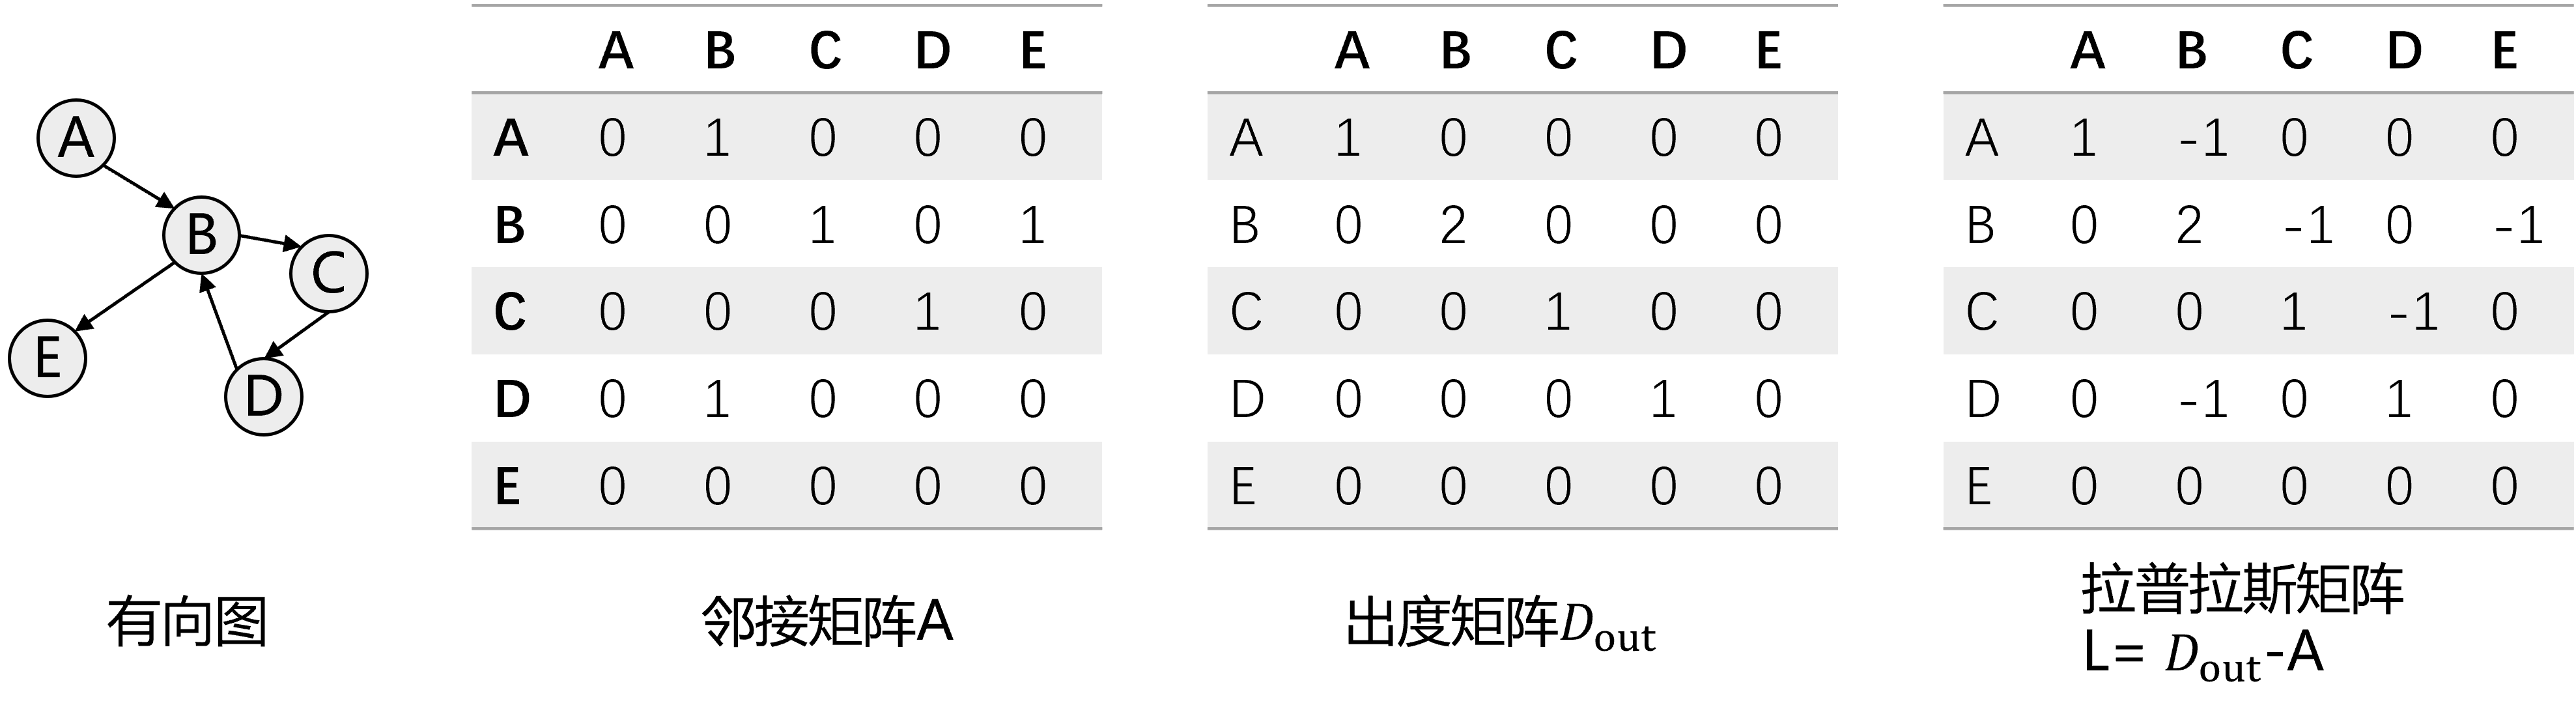
\includegraphics[width=0.95\textwidth]{figures/graph.png}
  \caption{有向图矩阵示例}\label{fig:graph}
\end{figure}

(1)邻接矩阵$A \in R^{N×N}$:用来表示图中节点之间关系的一种矩阵表示方法,如果存在从节点$v_i$指向节点$v_j$的边,那么$A[i][j] = 1$,如果不存在边,则$A[i][j] = 0$。(2)度矩阵$D \in R^{N×N}$:对角矩阵,用于表示图中每个节点的度(即与该节点相连的边的数量)。出度是从该节点出发的边的数量,入度是指向该节点的边的数量。度矩阵只有对角线上有值,对于节点$v_i$有$D[i][i] = \sum_j A_{ij}$,其他位置的元素都是0。对于有向图,可以分别构建入度矩阵$D_{in}$和出度矩阵$D_{out}$。(3)拉普拉斯矩阵$L \in R^{N×N} = D_{out} - A$:通过矩阵的形式描述了图的拓扑结构和性质,在图的传播和扩散问题中起到关键作用,通过特征值分解得到图的特征向量,有助于图的划分和聚类。

通过引入邻接矩阵和度矩阵,图卷积神经网络能够捕获图的拓扑结构信息,这是处理图数据的关键。该模型的输入$X \in R^{N×C}$为节点特征矩阵、$A \in R^{N×N}$为邻接矩阵,输出是一个特征矩阵$Z \in R^{N×F}$,表示学习到的每个节点的特征表示,$F$为模型自己定义的输出向量维度。下图\ref{fig:gcn}为图卷积神经网络结构图。
\begin{figure}[H]
  \centering
  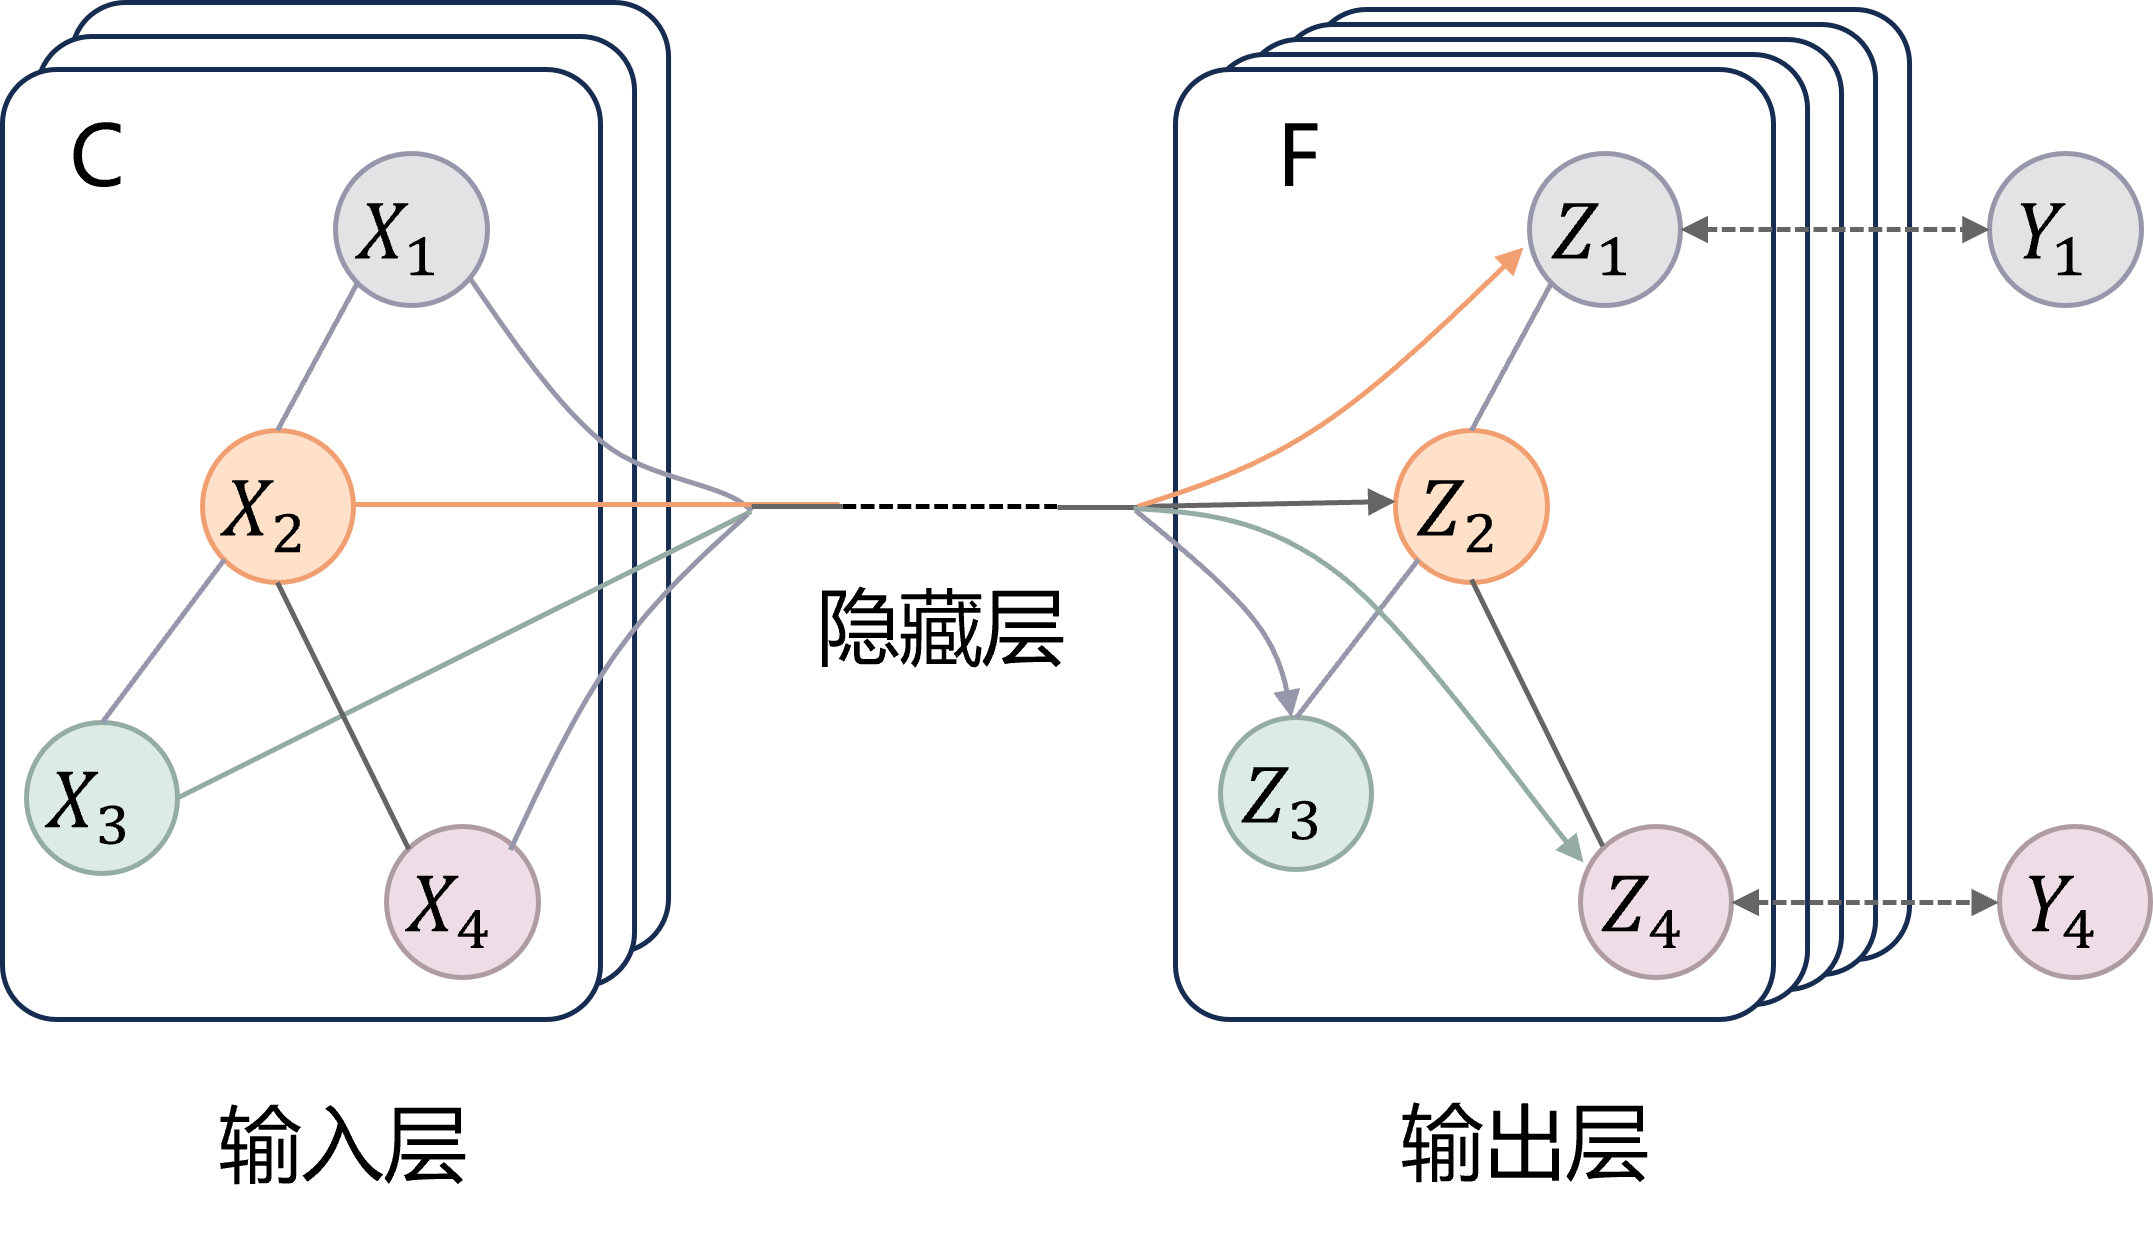
\includegraphics[width=0.55\textwidth]{figures/gcn.png}
  \caption{图卷积神经网络结构图}\label{fig:gcn}
\end{figure}

中间每一个图卷积层的输入都是邻接矩阵A和节点特征X,层与层之间的传播公式都可以写成\ref{e5.2};

\begin{equation}\label{e5.2}
  \begin{split}
    X^{l+1} = \sigma(\tilde{D}^{-\frac{1}{2}}\tilde{A}\tilde{D}^{-\frac{1}{2}}X^{l}W^{l})
  \end{split}
\end{equation}

其中:$X^{l}$ 表示第$l$层的节点特征矩阵。$W^{l}$是第 $l$层的参数,即可学习的权重矩阵。$\sigma$是激活函数,如ReLU。$\tilde{A} = A + I$,其中$I$是单位矩阵,表示给每个节点添加一条到自身的边,聚合时可以结合自身的特征消息。$\tilde{D}$是$\tilde{A}$的度矩阵,其公式为$\tilde{D[i][i]} = \sum_j \tilde{A_{ij}}$。对邻接矩阵$\tilde{A}$进行归一化操作$\tilde{D}^{-\frac{1}{2}}\tilde{A}\tilde{D}^{-\frac{1}{2}}$是为了信息传递的过程中保持特征矩阵$X$的原有分布,那些具有较低度的节点会对其邻居有较大的影响,而具有高度的节点会产生更小的影响因为他们的影响会被分散给很多的邻居节点。

\section{PDG表征方法具体实现}
\label{sec:PDGachieve}
在介绍具体实现之前,本节首先给出PDG表征方法的输入:经过\ref{subsec:Preprocess}小节的代码预处理阶段,得到示例代码片段\ref{fig:code}对应的程序依赖图,如图\ref{fig:pdgcode}所示。图中的实线表示节点之间的控制依赖,虚线表示节点之间的数据依赖。仔细分析三张图,其中图\ref{fig:pdg1}和图\ref{fig:pdg2}红框中节点11、12虽然位置有所改变,但是其边依赖均相同,因此可以视为完全相同的同构图;而图\ref{fig:pdg3}因为增加了一个if语句,图中也增加了一个节点,同时添加的红色的线表示新增的数据依赖、控制依赖。

\begin{figure}[htbp]
  \centering  %居中
  \subfigure[C语言代码片段1对应的PDG]{   %第一张子图
      \centering    %子图居中
      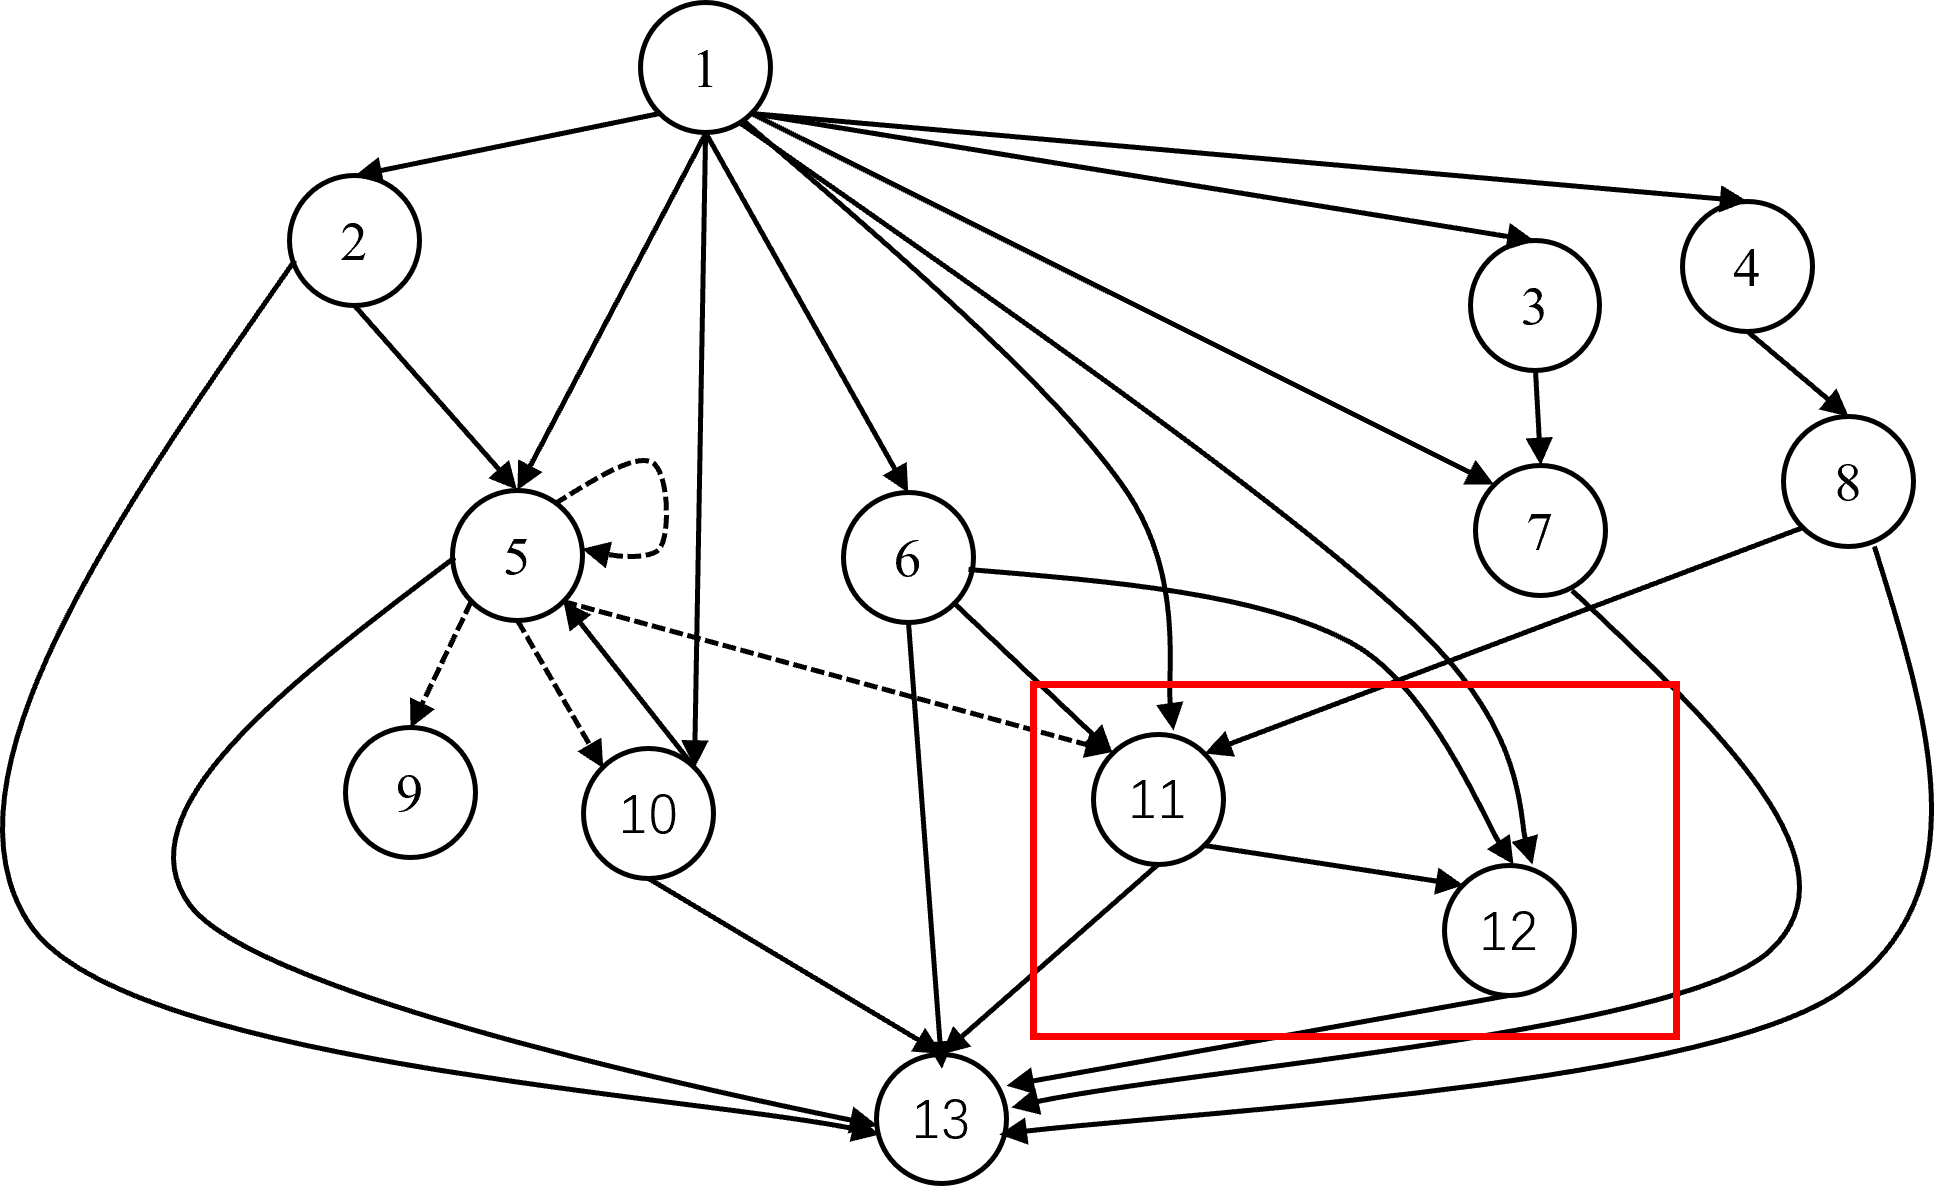
\includegraphics[width=0.3\textwidth]{figures/pdg1}  
      \label{fig:pdg1} %引用标签
  }
  \subfigure[C语言代码片段2对应的PDG]{ %第二张子图
      \centering    %子图居中
      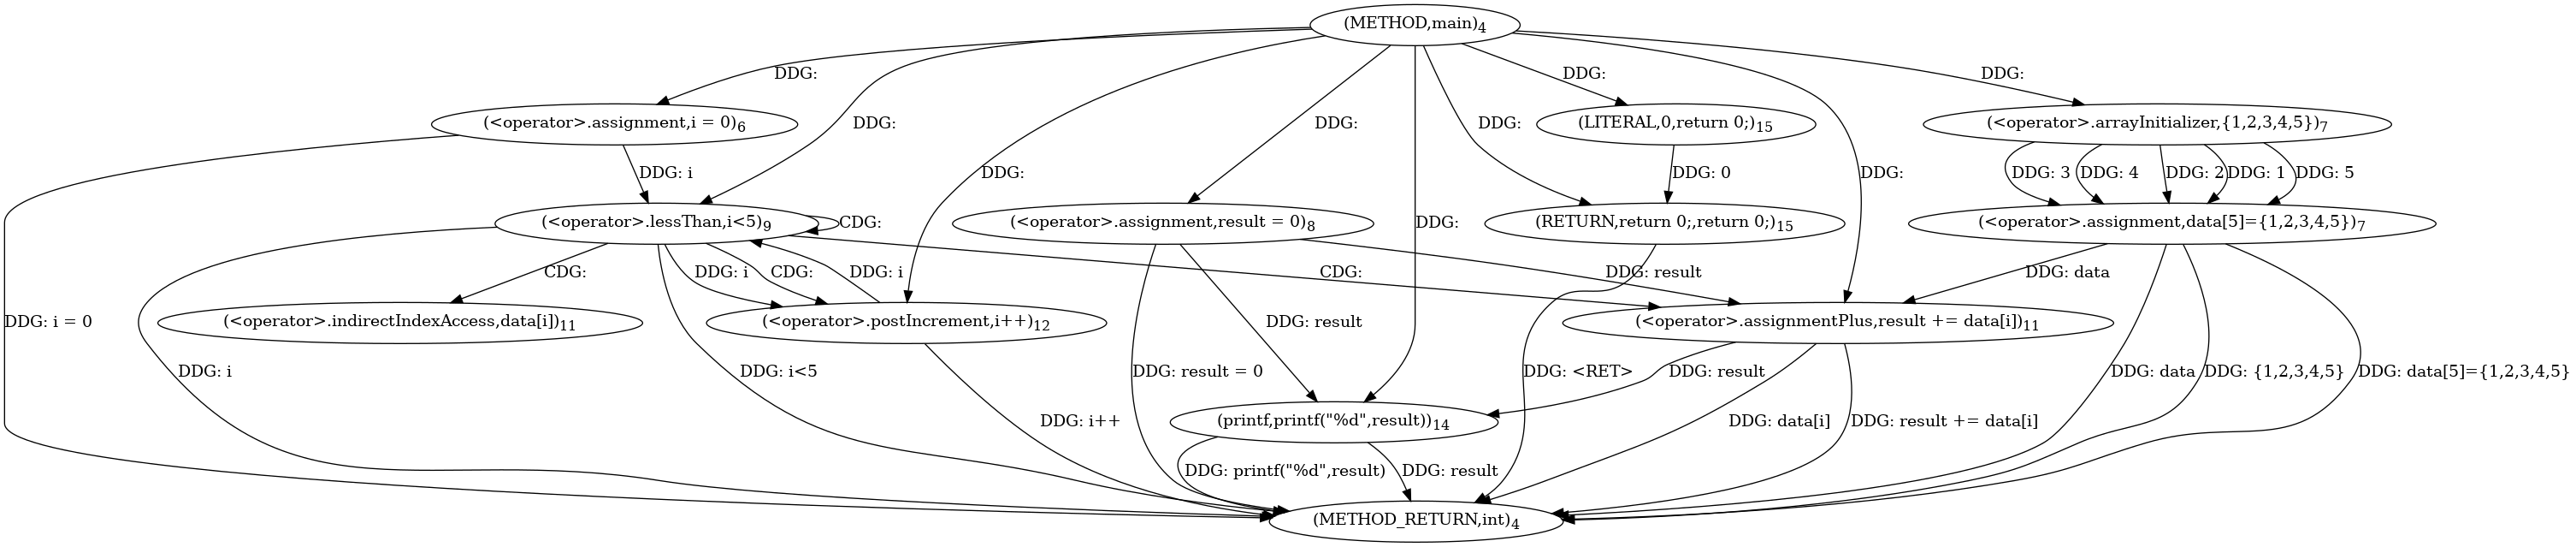
\includegraphics[width=0.3\textwidth]{figures/pdg2}
      \label{fig:pdg2} %引用标签
  }\subfigure[C语言代码片段3对应的PDG]{ %第二张子图
  \centering    %子图居中
  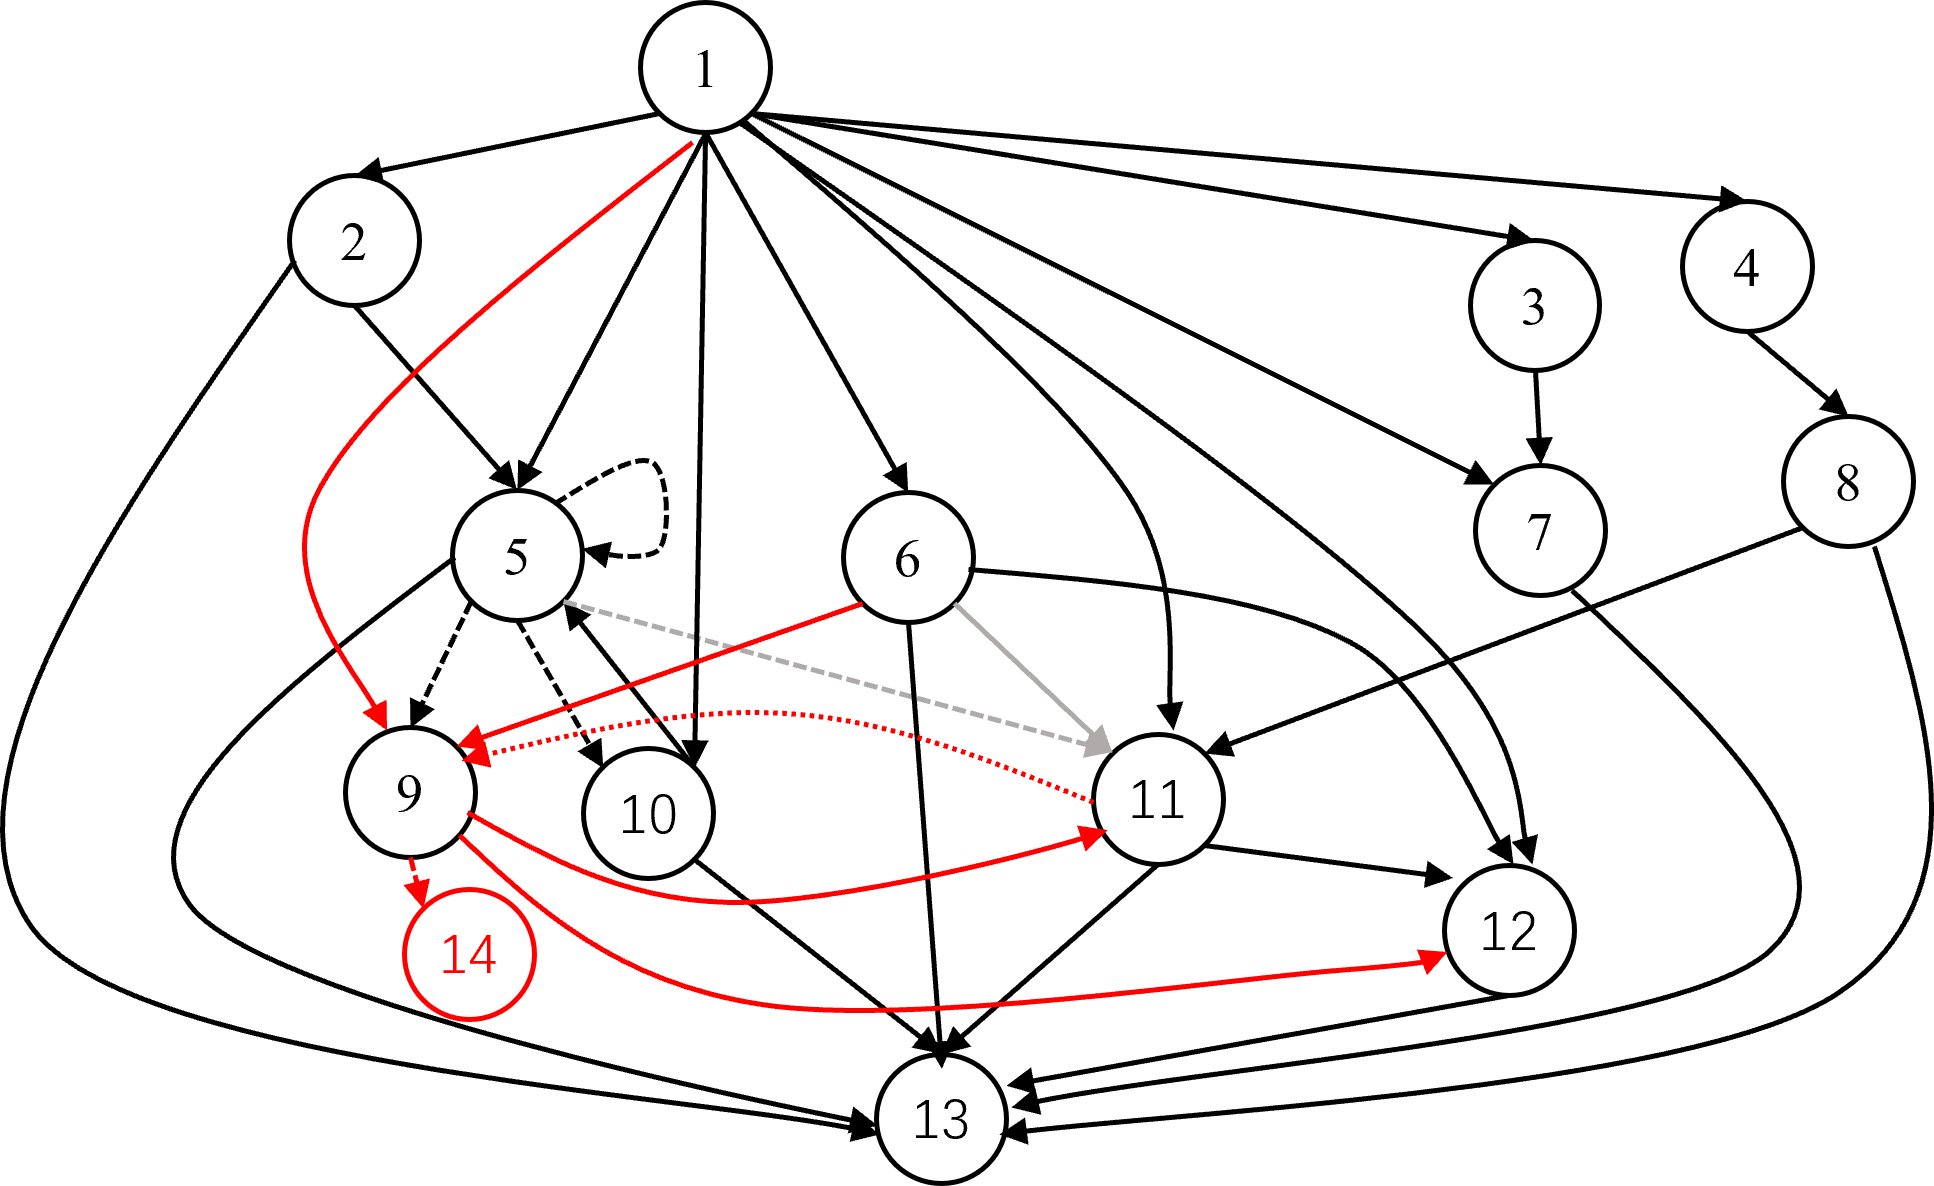
\includegraphics[width=0.3\textwidth]{figures/pdg3}
  \label{fig:pdg3} %引用标签
}
  \caption{示例源代码对应的程序依赖图}    %大图名称
  \label{fig:pdgcode}    %图片引用标记
\end{figure}

接下来,本章提出的基于图过滤的程序依赖图表征学习方法的实现如图\ref{fig:pdg}所示。该方法的输入是一对代码片段$C_{a},C_{b}$对应的程序依赖图,表示为$PDG_{a},PDG_{b}$,输出是$C_{a},C_{b}$对应的语义特征向量 $V_{a}^{PDG},V_{b}^{PDG}$,整体采用Siamese架构,两个子网络共享权值,从下到上,主要包括图过滤判断、图表征三个阶段。

\begin{figure}[H]
  \centering
  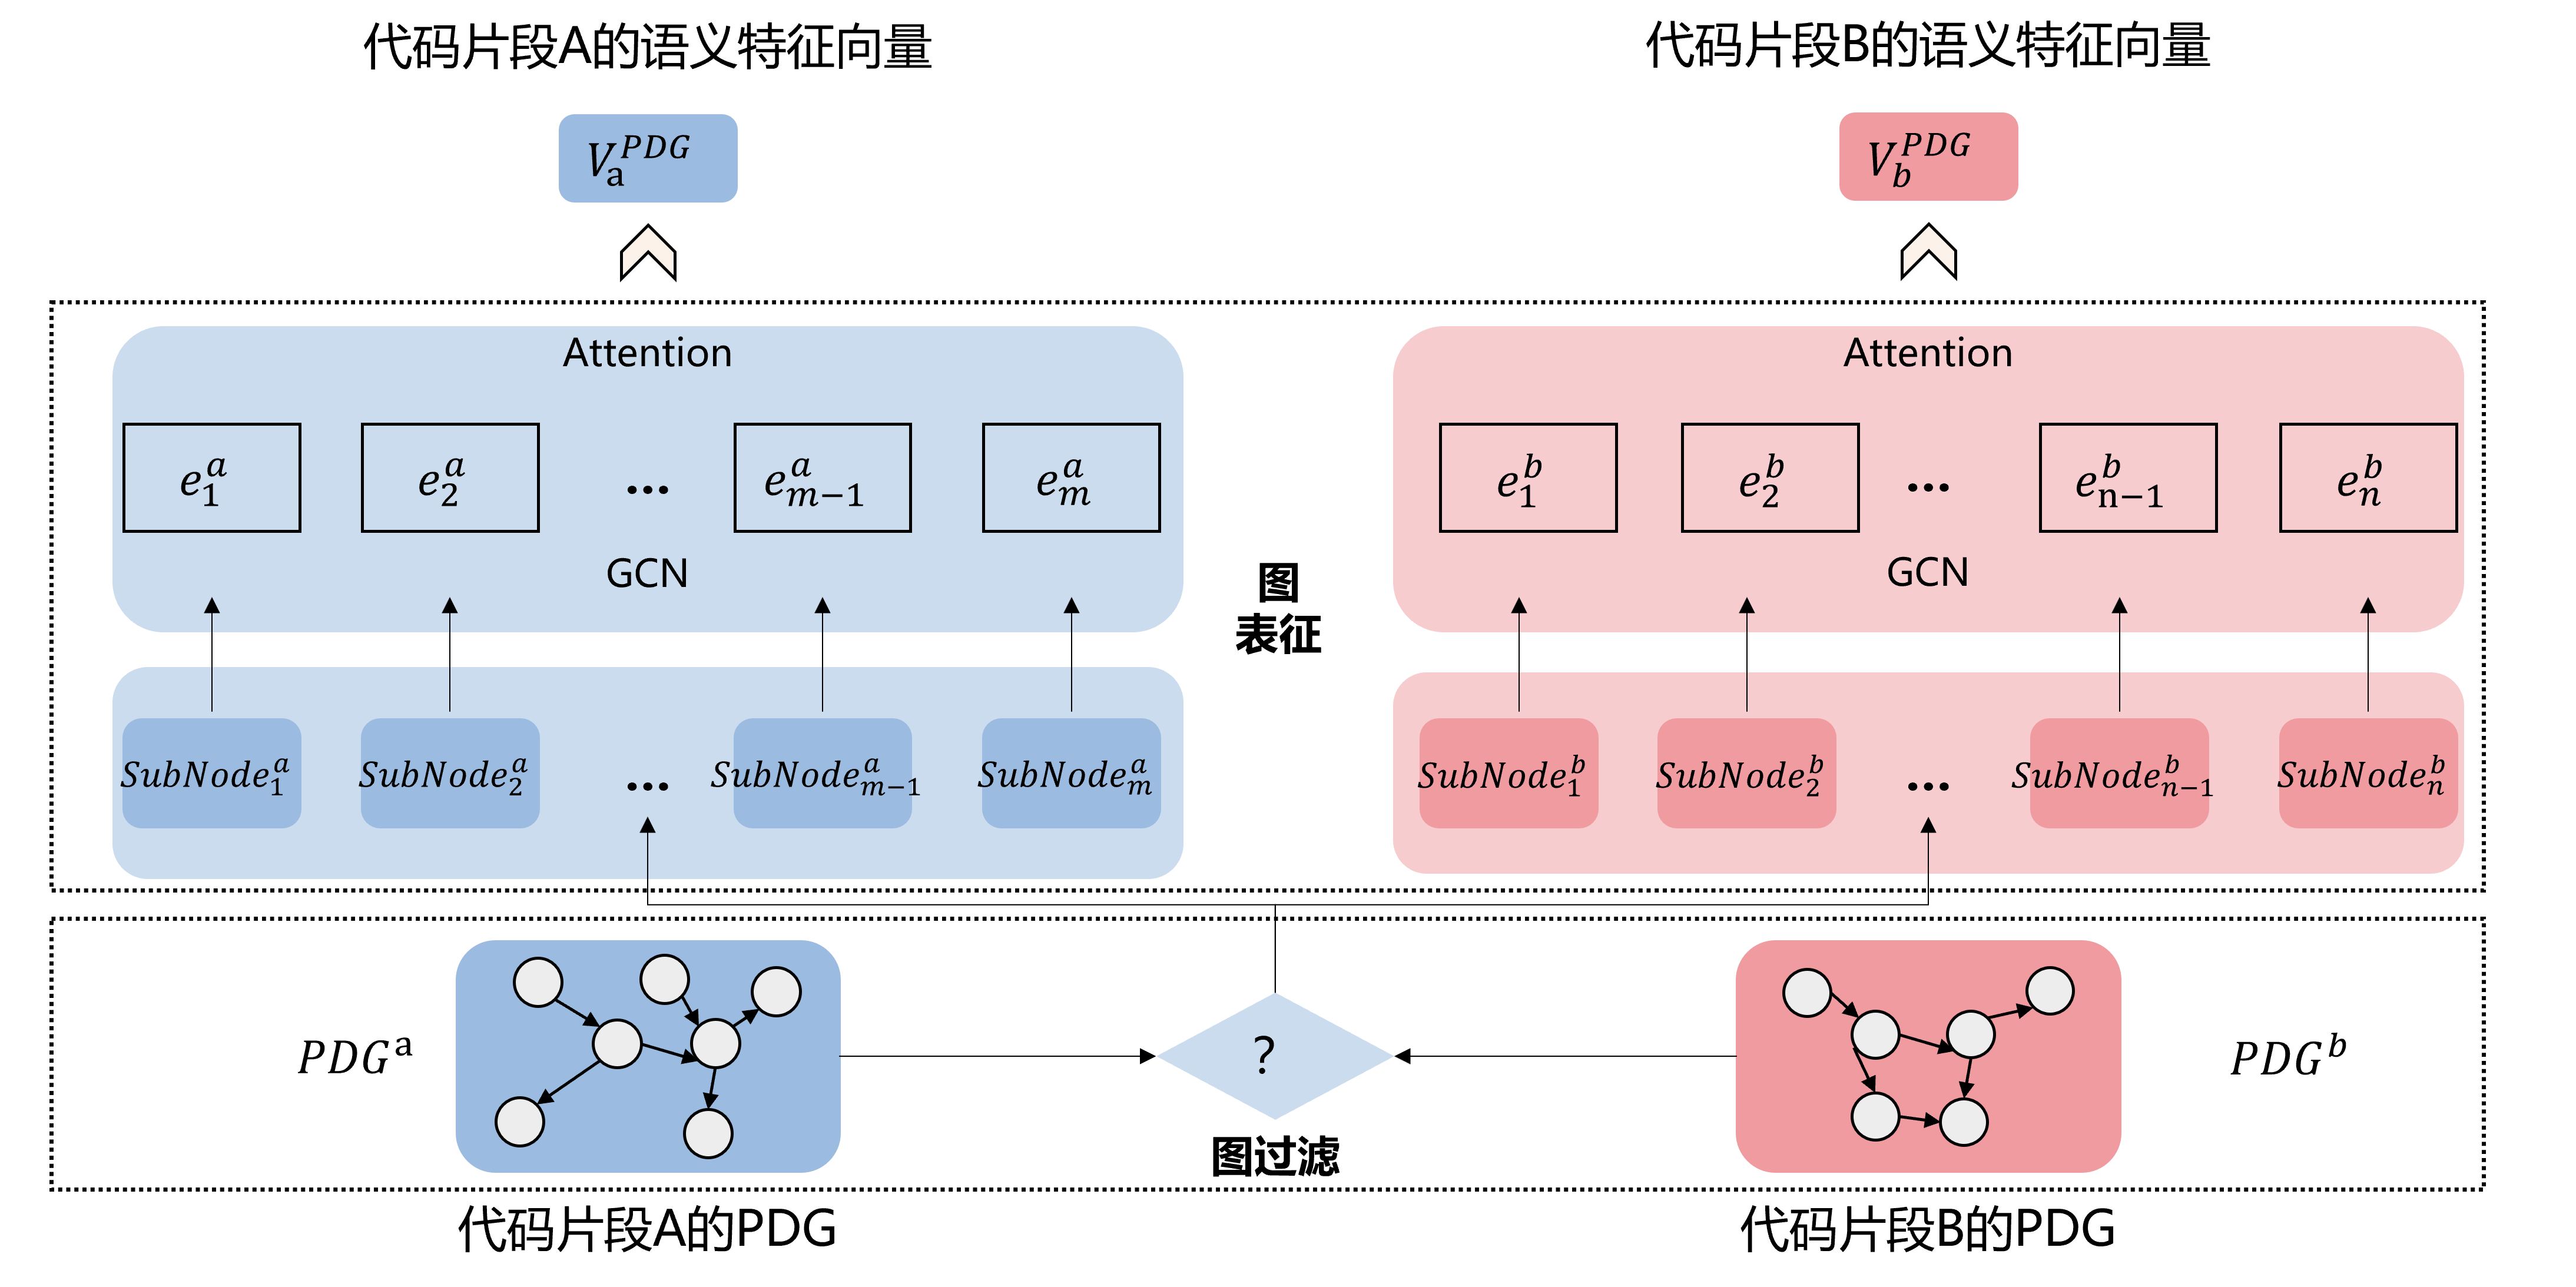
\includegraphics[width=0.9\textwidth]{figures/pdg.png}
  \caption{基于图过滤的程序依赖图表征学习方法实现}\label{fig:pdg}
\end{figure}

在图过滤阶段,将输入的PDG对进行过滤判定。首先对程序依赖图进行图结构约简,然后判断其有效行数是否大于6,是否存在子图同构,最后再判断两者的数值特征相似度是否大于阈值。如果顺利上述四个步骤,则该PDG对输入图表征模型。其过滤过程可以表达为公式\ref{e5.3}:

\begin{equation}\label{e5.3}
  \begin{split}
    \left(x_{1}^{a},x_{2}^{a},\ldots,x_{m}^{a}\right) = filter\_PDG \left(PDG_{a}\right)
  \end{split}
\end{equation}


在图表征模型,将PDG图作为输入,使用图卷积神经网络进行编码。处理过程分为两个步骤,如公式\ref{e5.4}所示。
\begin{equation}\label{e5.4}
  \begin{split}
    e_{1}^{aGCN},e_{2}^{aGCN},\ldots,e_{n}^{aGCN} = GCN\left(x_{1}^{a},x_{2}^{a},\ldots,x_{m}^{a}\right) \\
    V_{a}^{PDG} = Attention \left( e_{1}^{aGCN},e_{2}^{aGCN},\ldots,e_{n}^{aGCN} \right)
  \end{split}
\end{equation}

经过图卷积编码后,生成了$e_{i}^{aGCN}$,然后经过Attention层的总结后,生成了$V_{a}^{PDG}$作为代码片段$C_{a}$的最终图表示,即语义特征向量。
同样,可以使用相同的计算以通过图过滤判断的PDG作为输入为代码片段$C_{b}$计算$V_{b}^{PDG}$。

\section{实验验证}
\label{sec:PDGExperiment}
为了验证基于图过滤的程序依赖图表征学习方法的有效性,本节开展实验验证。首先,介绍了实验的具体设计,接着对子树划分、树表征模型进行消融实验。

\subsection{实验设计}
\label{sec:PDGDesign}

本节使用与\ref{sec:TokenExperiment}节中同样的实验环境、数据集对基于图过滤的程序依赖图表征学习方法进行对比实验。使用代码分析工具Joern获取数据集中代码片段的程序依赖图,然后使用图卷积神经网络训练图嵌入,并将嵌入向量大小设置为128。同样选取常用的精确率(Precision)、召回率(Recall)、F1值作为评估指标。

\subsection{实验结果}
\label{subsec:PDGResult}

(1) 图过滤机制的实验结果

为了探究图过滤机制对程序依赖图表征实验结果的影响,本文针对图过滤阶段中的:规模过滤、数值特征过滤两种策略进行了实验验证。其中,将规模过滤用PDG-size表示,数值特征过滤用PDG-Number表示,两种过滤策略均使用用PDG-All表示。本实验采取单一变量原则,仅修改图过滤策略,后续程序依赖图的编码采用相同的图卷积神经网络。具体实验结果如表\ref{tab:graph}所示。

\begin{table}[htp]
  \centering
  \caption{图过滤机制对实验结果的影响} 
  \label{tab:graph}
  \begin{tabular*}{0.9\textwidth}{@{\extracolsep{\fill}}ccccc}
  \toprule
   \multirow{2}{*}{图过滤策略} & \multirow{2}{*}{过滤后剩余PDG对} & \multicolumn{3}{c}{POJ104} \\
  \cmidrule{3-5} 
   & & 准确率P(\%) & 召回率R(\%) & F1值(\%)  \\ 
  \midrule
    PDG-Size		   & 6072	  &87.63	 &88.75		&88.19 \\
    PDG-Number		 & 7952	  &85.32   &82.65   &83.96 \\
    PDG-All		     & 5000	  &89.53   &81.71	 &85.44 \\
  \bottomrule
  \end{tabular*}
\end{table}

从表\ref{tab:graph}可以看出,本文使用的图过滤机制可以过滤掉大多数的候选PDG对。初始PDG对总数目为50000,经过过滤后的PDG对占原来PDG对数的比例大致在15\%以下,这意味着图过滤机制可以排除大部分候选PDG对,大大减少后续图表征模型的工作负担。同时面向代码克隆检测任务,不同PDG过滤策略处理后,其准确率、召回率、F1值相差不大,深究其原因,可能是在相似的图规模作为输入的情况下,图卷积模型训练策略没有差异,其代码信息表征能力也没有很大差异。因此,得出以下结论:本章提出的图过滤机制,面向代码克隆检测任务具有一定优势。考虑到后续输入图卷积神经网络的规模无需过大,避免给图表征模型带来过大训练压力,最终选择两种图过滤策略均使用的方法PDG-All作为图过滤机制。

(2) 图表征模型的实验结果

为了探究图表征模型对实验结果的影响,本文将图卷积神经网络与Weisfeiler-Lehman算法进行对比,结果如表\ref{tab:tree2}所示。其中Weisfeiler-Lehman(WL)算法是一种基于子图同构的检测算法,它的关键思想是通过对每个节点的所有相邻节点的标签排序,然后将标签根据某一映射压缩为新的更短的标签值来反映图中局部结构,通过统计两个图中相同标签值得数目判断两个图得相似度大小\cite{articleWL}。

其中,图卷积神经网络基于Pytorch1.10实现,其参数设置为:\ding{172} 图过滤:采用PDG-All的过滤方法。\ding{173} 表征模型的隐藏层维度设置为128,模型使用二元交叉熵作为损失函数,使用Adam优化器来训练模型参数,其中,学习率Learning\_rate设置为0.001,Dropout为0.5,训练批次Epochs为50,批处理大小Batch\_size为32,阈值Threshold为0.5,当相似度超过0.5,输入的代码对被判定为真克隆对,否则被判定为假克隆对。参数的确定是通过多次调试后选择最优参数作为最后的结果。\ding{174} WL算法对每个节点按照其类型进行数值化处理,采用(声明节点,赋值节点,控制节点,函数调用节点,其他节点)格式进行数值化。


\begin{table}[htp]  
  \centering  
  \caption{图表征模型对实验结果的影响}   
  \label{tab:graph2}
  %\renewcommand{\arraystretch}{1.1}  
  \begin{tabular*}{0.9\textwidth}{@{\extracolsep{\fill}}cccc}  
  \toprule  
  表征方法 & 准确率P(\%) & 召回率R(\%) & F1值(\%)  \\  
  \midrule
  Weisfeiler-Lehman图核算法  & 92.21	  & 52.13	 & 66.61		\\  
  图卷积神经网络		         & 89.53		&81.71		&85.44\\ 
  \bottomrule  
  \end{tabular*}  
\end{table}

基于对表\ref{tab:graph2}数据的分析,可以得到以下结论:(1)在对图进行表征的过程中,WL算法的准确率比图卷积神经网络更高。深究其原因,WL算法通过迭代更新节点的标签,可以捕获图的结构信息,算法实现简单,准确率高。(2)WL算法的召回率只有52.13\%。深究其原因,WL算法迭代过程中过于关注图结构信息,反而忽略了节点自身的特征信息,同时对迭代次数敏感,次数过少无法充分捕获图的结构信息。(3)综合F1值,图卷积神经网络对程序依赖图表征效果优势明显,面向代码克隆检测任务的实验结果更优秀。深究其原因,图卷积神经网络能够自动学习图节点的表示,同时聚合邻居节点的信息来更新节点的特征,从而捕获图结构信息、节点特征信息。因此,在图维度的代码表征模型选取上,本文更倾向于图卷积神经网络GCN。

(3)PDG表征可视化

为了更直观地展示本文提出的图过滤的PDG表征学习方法的有效性,本实验同样使用t-SNE技术将高维语义特征向量可视化。按照预先设定的参数,图表征学习后生成的张量维度是128,本实验采用t-SNE技术将128维的张量转换为2维,得到的样本表征结果如图\ref{fig:originthree}所示。

\begin{figure}[H] 
  \centering  %居中
  \subfigure[初始向量可视化]{   %第一张子图
      \centering    %子图居中
      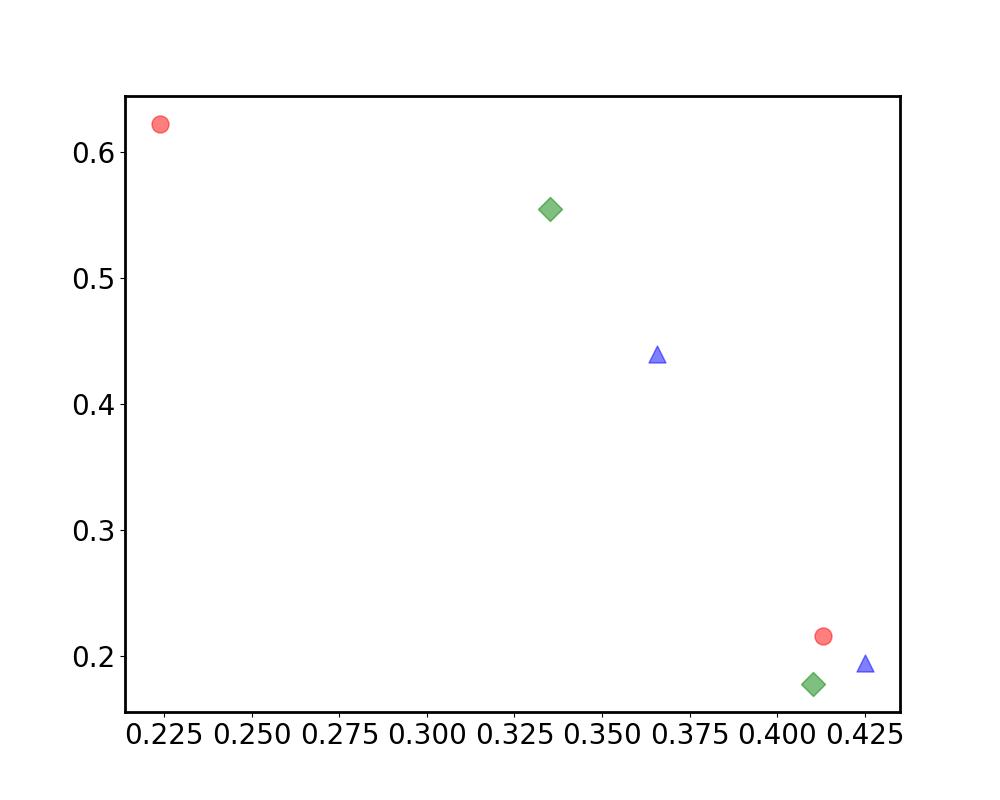
\includegraphics[width=0.45\textwidth]{figures/origin.png} 
      \label{fig:originp} %引用标签
  }
  \subfigure[语义特征向量可视化]{ %第二张子图
      \centering    %子图居中
      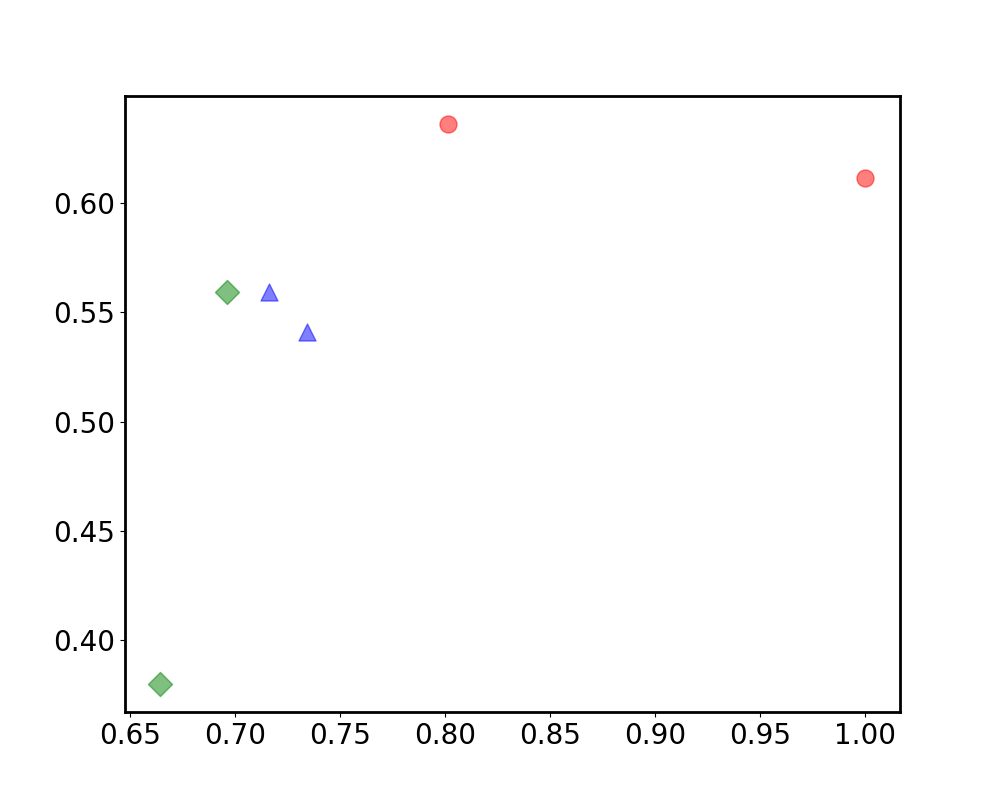
\includegraphics[width=0.45\textwidth]{figures/origin3.png}
      \label{fig:origin3} %引用标签
  }p
  \caption{t-SNE技术降维后的语义特征向量可视化结果}    %大图名称
  \label{fig:originthree}    %图片引用标记
\end{figure}

如图\ref{fig:originthree}所示,\ref{fig:originp}和\ref{subsec:TokenResult}可视化实验中采用的代码片段相同,而\ref{fig:origin3}中,向量空间的所有点是代码片段通过图表征学习后得到的语义特征向量可视化结果。可以看到互为真克隆对的代码片段在经过图表征模型训练后语义更接近,距离更小。但是其中有一个绿色菱形与蓝色三角距离过近,探究其原因,可能是其代码片段虽然带有不同的标签,但生成的程序依赖图相似,在图表征后得到的语义特征向量距离过近,可视化结果来看,其距离更接近。

\section{本章小结}
\label{sec:Summary5}
本章主要对RLCCD中基于图过滤的程序依赖图表征学习方法的设计与实现进行详细阐述。首先介绍了程序依赖图维度的研究动机,其次介绍了程序依赖图表征学习的方法设计,具体论述了其整体框架、图过滤、图表征学习,接着开展实验验证,结果表明了此方法的有效性和模型的准确性。




\chapter{特征融合及RLCCD框架验证}
\label{chap:fusion}
本章主要对面向代码克隆检测的多维源代码表征方法整体框架RLCCD进行介绍,同时进行实验评估及验证。具体地,RLCCD是由上述基于预训练辅助模型的Token表征学习、基于子树划分的抽象语法树表征学习、基于图过滤的程序依赖图表征学习方法三种维度融合形成并进行实现的表征方法,最后通过与SourcererCC、ASTNN、SCDetector进行对比实验以验证该框架的有效性。
\section{特征融合}
特征融合

特征融合方法是指将不同来源或不同层次的特征进行组合,合并成一个比输入特征更具有判别能力的特征,该多维特征能够在低维空间中高效计算实体和关系的语义联系,提高特征的表达能力和分类效果,有利于下游代码克隆检测任务的学习。

\section{RLCCD框架验证}
本文的实验设计主要围绕以下4 个方面的研究问题:

• RQ1:本文提出的预训练辅助模型策略是否优于基线方法?(见3.3 节)

• RQ2:本文提出的子树划分策略是否优于基线方法?(见4.3 节)

• RQ3:本文提出的图过滤策略能否优于基线方法?(见5.3 节)

• RQ4:与现有代码克隆检测工具相比,RLCCD 表现如何?

\subsection{实验设置}
(1)系统环境

本章实验均在Ubuntu 16.04 LTS(64位)系统下进行。


(2)实验数据集

本章实验部分采用的数据集为代码克隆检测领域常见的基准集POJ104,该数据集是一个基于C语言构建的大型数据集,包含了104个编程问题以及学生提交的对应问题的不同C语言源代码,在该数据集中,针对同一问题的不同源解法的代码被视为一个克隆对。

首先通过筛选,得到51485个源代码样本,然后随机生成50000个代码克隆对,其中包含5200个真克隆对,44800个假克隆对。依据随机种子将数据集按照3:1:1划分为训练集、测试机、验证集,其中的正负样本数如下表。


\subsection{对比工具}
在对比整个方法的效果时,本文选取开源的SourcererCC、ASTNN、SCDetector方法进行比较。

SourcererCC:SourcererCC是一种相对较新的基于token的克隆检测工具。该工具通过词袋模型,把收集的数据全部编码成词频信息,后将代码行转换成一个由词频构成的向量,通过向量的比较获取相似度。

ASTNN:一种基于神经网络的源代码表示方法。它将整个抽象语法树AST分解成一系列小型语句子树,并通过捕获语句的词法和语法信息将语句子树分别编码为向量,最后采用了RNN模型生成代码片段的向量表示。ASTNN方法完整保留了抽象语法树的结构信息,能够检测到所有类型的代码克隆。

SCDetector:是基于令牌和基于图的方法的结合。给定一个方法源代码,我们首先生成CFG,然后应用中心性分析将图转换为某些语义标记(即具有图细节的标记)。最后,这些语义标记被馈送到Siamese网络中,以训练模型并使用它来检测代码克隆对。

\subsection{RLCCD性能评估实验结果}

对比实验:体现框架的有效性


\begin{table}
  \centering
  \caption{RLCCD实验结果} %\label{tab:category}
  \begin{tabular*}{0.9\textwidth}{@{\extracolsep{\fill}}cccc}
  \toprule
    对比			&P		&R		&F1 \\
  \midrule
    SourcererCC			&0.xx	&0.xx		&0.xx \\
    ASTNN			&0.xx		&0.xx		&0.xx \\
    SCDetector			&0.xx	&0.xx		&0.xx \\
    RLCDD			&0.xx		&0.xx		&0.xx \\
  \bottomrule
  \end{tabular*}
\end{table}

\section{本章小结}
本章节主要对RLCCD框架进行了实验验证,以验证RLCCD的XXX能力。





\backmatter

% 结论
%%
% The BIThesis Template for Graduate Thesis
%
% Copyright 2020-2023 Yang Yating, BITNP
%
% This work may be distributed and/or modified under the
% conditions of the LaTeX Project Public License, either version 1.3
% of this license or (at your option) any later version.
% The latest version of this license is in
%   http://www.latex-project.org/lppl.txt
% and version 1.3 or later is part of all distributions of LaTeX
% version 2005/12/01 or later.
%
% This work has the LPPL maintenance status `maintained'.
%
% The Current Maintainer of this work is Feng Kaiyu.

\begin{conclusion}

本文采用……。{\color{blue}(结论作为学位论文正文的最后部分单独排写,但不加章号。结论是对整个论文主要结果的总结。在结论中应明确指出本研究的创新点,对其应用前景和社会、经济价值等加以预测和评价,并指出今后进一步在本研究方向进行研究工作的展望与设想。结论部分的撰写应简明扼要,突出创新性。)}

\end{conclusion}

% 参考文献
%%
% The BIThesis Template for Graduate Thesis
%
% Copyright 2020-2023 Yang Yating, BITNP
%
% This work may be distributed and/or modified under the
% conditions of the LaTeX Project Public License, either version 1.3
% of this license or (at your option) any later version.
% The latest version of this license is in
%   http://www.latex-project.org/lppl.txt
% and version 1.3 or later is part of all distributions of LaTeX
% version 2005/12/01 or later.
%
% This work has the LPPL maintenance status `maintained'.
%
% The Current Maintainer of this work is Feng Kaiyu.

%
% 如无特殊需要,本页面无需更改


\begin{bibprint}
  \printbibliography[heading=none,notcategory=mypub,resetnumbers=true]
\end{bibprint}


% 附录
% %%
% The BIThesis Template for Graduate Thesis
%
% Copyright 2020-2023 Yang Yating, BITNP
%
% This work may be distributed and/or modified under the
% conditions of the LaTeX Project Public License, either version 1.3
% of this license or (at your option) any later version.
% The latest version of this license is in
%   http://www.latex-project.org/lppl.txt
% and version 1.3 or later is part of all distributions of LaTeX
% version 2005/12/01 or later.
%
% This work has the LPPL maintenance status `maintained'.
%
% The Current Maintainer of this work is Feng Kaiyu.

\begin{appendices}
  \chapter{费马大定理的证明}
  关于此,我确信已发现了一种美妙的证法,可惜这里空白的地方太小,写不下。

  \chapter{Maxwell Equations}
  因为在柱坐标系下,$\overline{\overline\mu}$是对角的,所以Maxwell方程组中电场$\bf
  E$的旋度

  所以$\bf H$的各个分量可以写为:
  \begin{subequations}
    \begin{eqnarray}
      H_r=\frac{1}{\mathbf{i}\omega\mu_r}\frac{1}{r}\frac{\partial
        E_z}{\partial\theta } \\
      H_\theta=-\frac{1}{\mathbf{i}\omega\mu_\theta}\frac{\partial E_z}{\partial r}
    \end{eqnarray}
  \end{subequations}

  同样地,在柱坐标系下,$\overline{\overline\epsilon}$是对角的,所以Maxwell方程组中磁场$\bf
  H$的旋度
  \begin{subequations}
    \begin{eqnarray}
      &&\nabla\times{\bf H}=-\mathbf{i}\omega{\bf D}\\
      &&\left[\frac{1}{r}\frac{\partial}{\partial
          r}(rH_\theta)-\frac{1}{r}\frac{\partial
          H_r}{\partial\theta}\right]{\hat{\bf
          z}}=-\mathbf{i}\omega{\overline{\overline\epsilon}}{\bf
        E}=-\mathbf{i}\omega\epsilon_zE_z{\hat{\bf z}} \\
      &&\frac{1}{r}\frac{\partial}{\partial
        r}(rH_\theta)-\frac{1}{r}\frac{\partial
        H_r}{\partial\theta}=-\mathbf{i}\omega\epsilon_zE_z
    \end{eqnarray}
  \end{subequations}

  由此我们可以得到关于$E_z$的波函数方程:
  \begin{eqnarray}
    \frac{1}{\mu_\theta\epsilon_z}\frac{1}{r}\frac{\partial}{\partial r}
    \left(r\frac{\partial E_z}{\partial r}\right)+
    \frac{1}{\mu_r\epsilon_z}\frac{1}{r^2}\frac{\partial^2E_z}{\partial\theta^2}
    +\omega^2 E_z=0
  \end{eqnarray}

  \chapter{要求}

  \textcolor{blue}{
  有些材料编入文章主体会有损于编排的条理性和逻辑性,或有碍于文章结构的紧凑和突出主题思想等,这些材料可作为附录另页排在参考文献之后,也可以单编成册。下列内容可作为附录:
  }
  \begin{enumerate}
    \item \textcolor{blue}{为了整篇论文材料的完整,但编入正文有损于编排的条理性和逻辑性的材料,这一类材料包括比正文更为详尽的信息、研究方法和技术等更深入的叙述,以及建议可阅读的参考文献题录和对了解正文内容有用的补充信息等;}
    \item \textcolor{blue}{ 由于篇幅过大或取材的复制资料不便于编入正文的材料; }
    \item \textcolor{blue}{ 不便于编入正文的罕见珍贵资料; }
    \item \textcolor{blue}{ 一般读者无须阅读,但对本专业同行有参考价值的资料; }
    \item \textcolor{blue}{ 某些重要的原始数据、推导、计算程序、框图、结构图、注释、统计表、计算机打印输出件等; }
  \end{enumerate}

  \section{一级标题}
  \subsection{二级标题}
\end{appendices}


% 个人成果
% 1. 在 `./reference/pub.bib` 中添加数据。
% 2. 在下方 `\addpubs` 添加该文献(参考下方示例)。

% **注意:如果发现渲染出来的文献编号不正确,请使用 `latexmk -c` 清除缓存后重新编译。**

\begin{publications}

  \addpubs{myCiteKey,myCiteKey2,dummy:1,dummy:2}

  % 主要针对硕士生
  \printbibliography[heading=none,category=mypub,resetnumbers=true]

  % 如果想要分为多个列表,可以使用以下的命令。
  % 主要针对博士生。
  % \pubsection{文章}
  %
  % \printbibliography[heading=none,type=article,category=mypub,resetnumbers=true]{}
  %
  % \pubsection{一些书}
  %
  % \printbibliography[heading=none,type=book,category=mypub,resetnumbers=true,notkeyword=dummy]{}
  %
  % \pubsection{另一些书}
  %
  % \printbibliography[heading=none,type=book,category=mypub,keyword=dummy,resetnumbers=true]{}

\end{publications}



% 致谢
\begin{acknowledgements}


\end{acknowledgements}

% 个人简介(仅博士生需要此项)
% %%
% The BIThesis Template for Graduate Thesis
%
% Copyright 2020-2023 Yang Yating, BITNP
%
% This work may be distributed and/or modified under the
% conditions of the LaTeX Project Public License, either version 1.3
% of this license or (at your option) any later version.
% The latest version of this license is in
%   http://www.latex-project.org/lppl.txt
% and version 1.3 or later is part of all distributions of LaTeX
% version 2005/12/01 or later.
%
% This work has the LPPL maintenance status `maintained'.
%
% The Current Maintainer of this work is Feng Kaiyu.

\begin{resume}

本人…。

\textcolor{blue}{
  硕士学位论文不必提供作者简介。博士学位论文应该提供作者简介,主要包括:姓名、性别、出生年月、民族、出生地;简要学历、工作经历(职务);攻读学位期间取得的其他研究成果或奖励。
}

\end{resume}


% 加入目录
\end{document}
